\documentclass[11pt]{article}
\usepackage{cmap}
\usepackage[T1]{fontenc}
\usepackage{lmodern}
\usepackage[margin=1in]{geometry}
\usepackage{amsmath,amssymb}
\usepackage{graphicx}
\graphicspath{{./}{figures/}}
\usepackage{hyperref}
\usepackage{natbib}
\usepackage{booktabs}
\usepackage{siunitx}
% Parameters of the project. Python reads this file with params.py, LaTeX reads it with \input.
% One macro per line; names contain letters only. Change a number here and "make" reruns what depends on it.

% --- Gray-Scott model and grid (src/simulation) ---
\newcommand{\Fval}{0.018}
\newcommand{\kval}{0.055}
\newcommand{\Duval}{2e-5}
\newcommand{\Dvval}{1e-5}
\newcommand{\Lval}{2.5}
\newcommand{\gridn}{1024}
\newcommand{\dtval}{1.0}

% --- Independent ensembles (Table 1): random-number seed bases ---
\newcommand{\SeedOne}{1000}
\newcommand{\SeedTwo}{9000}
\newcommand{\SeedThree}{20000}

% --- Ensemble design (Table 1): realisations per ensemble and burn-in in time steps ---
\newcommand{\RunsOne}{1000}
\newcommand{\BurninOne}{7000}
\newcommand{\RunsTwo}{1000}
\newcommand{\BurninTwo}{7000}
\newcommand{\RunsThree}{1000}
\newcommand{\BurninThree}{7000}

\newcommand{\SpacingOne}{100}
\newcommand{\SpacingTwo}{100}
\newcommand{\SpacingThree}{1000}
\newcommand{\SettleSteps}{3800}
\newcommand{\PatchHalf}{80}
\newcommand{\SettleSeed}{0}
\newcommand{\MasterFrames}{500}
\newcommand{\LifeSteps}{10000}

% --- Further simulations (frames per run, realisations, steps; from the validated rerun) ---
\newcommand{\FramesRemaining}{500}
\newcommand{\FramesShapeTail}{400}
\newcommand{\FramesShapeStab}{200}
\newcommand{\FramesMinDist}{500}
\newcommand{\FramesConfound}{300}
\newcommand{\FramesResLow}{400}
\newcommand{\FramesResHigh}{400}
\newcommand{\CountReal}{12}
\newcommand{\CountSteps}{15000}
\newcommand{\ThreeVarTarget}{100000}
\newcommand{\ThreeVarBurnin}{7000}
\newcommand{\FramesCentroid}{500}
\newcommand{\FramesVRate}{500}
\newcommand{\FramesPosGap}{400}
\newcommand{\FramesTouching}{400}
\newcommand{\FramesDensity}{30}
\newcommand{\FramesDealias}{400}
\newcommand{\BootReps}{2000}
\newcommand{\CmiJobs}{12}
\newcommand{\NullReps}{48}
\newcommand{\JacobianFrame}{454}
\newcommand{\DepthStride}{10}
\newcommand{\DivRefA}{10000}
\newcommand{\DivRefB}{319000}
\newcommand{\DivRefC}{469000}
\newcommand{\DivBranch}{6000}
\newcommand{\SnapshotFrame}{250}
\newcommand{\CmiSubsamples}{20}
\newcommand{\CmiNullSubsamples}{3}
\newcommand{\CmiNSub}{8000}
\newcommand{\CmiTrials}{300}

\input{results}
% Helpers for numbers that come from the code (build/initialize.tex and build/results.tex).
% A value the code could not compute is written as nan; it prints as "n/a" (make check lists every such macro).
% \rr and \nn take a macro name (\ifx compares it with the macro \nanvalue, so this also works inside captions).
\newcommand{\nanvalue}{nan}
\newcommand{\rr}[2]{\ifx#2\nanvalue\text{n/a}\else\num[round-mode=places,round-precision=#1]{#2}\fi}  % \rr{places}{\Macro}: rounded, with a proper minus
\newcommand{\nn}[1]{\ifx#1\nanvalue\text{n/a}\else{\sisetup{group-separator={,}}\num{#1}}\fi}        % integer with comma grouping

\usepackage{microtype}\DisableLigatures[-]{encoding=*,family=tt*}
\usepackage{array}
\usepackage{longtable}

\newcommand{\eps}{\varepsilon}
\newcommand{\bB}{\boldsymbol{B}}

% Numbering conventions for the electronic supplementary material, following
% the usual Royal Society Publishing practice of prefixing all supplementary
% figures, tables, and equations with "S" so they cannot be confused with the
% main text's own numbering (main-text figures are 1-9 at time of writing).
\renewcommand{\thefigure}{S\arabic{figure}}
\renewcommand{\thetable}{S\arabic{table}}
\renewcommand{\theequation}{S\arabic{equation}}
\renewcommand{\thesection}{S\arabic{section}}

\title{Electronic Supplementary Material for:\\[4pt]
\large Does a Flux-Defined Markov Blanket Screen Self-Replicating Gray--Scott Spots?\\
A Computational Test of a Blanket Condition from the Free Energy Principle}
\author{John E. Pearson\\
Los Alamos, NM 87544}
\date{\today}

% Labels of the main text (\newlabel lines copied from paper.aux; see build.sh). A plain .tex file is read
% instead of paper.aux, so that this document compiles on its own.
\makeatletter
\input{paper_labels}
\makeatother

\begin{document}
\maketitle

\noindent This document provides the full simulation methods and the detailed
statistical tests, robustness checks, and confound checks supporting the
results summarised in the main text. Every check here is referenced from the
main text at the point where its headline result is reported; the main text
is intended to stand on its own, and this document exists to let a reader
verify, reproduce, or scrutinise any specific claim without interrupting the
main argument.

\tableofcontents

\section*{Map of Claims, Evidence and Remaining Qualifications}
\label{sec:S_claimsmap}

\begin{longtable}{p{3.6cm}p{5.0cm}p{5.6cm}}
\toprule
Claim (main text) & Supporting analysis & Remaining qualification \\
\midrule
\endhead
Flux does not screen $I$ from $E$ (\S\ref{sec:conditional_independence}) & Linear partial correlation (single trajectory and ensemble, \S\ref{sec:ci_ensemble}); nonlinear CMI with $z$-scored variables and two nulls (\S\ref{sec:ci_cmi}); level-set individuation (\S\ref{sec:S_levelset}) & Tests flux-defined blanket on coarse-grained $I$, $E$; naive intervals overstate precision (\S\ref{sec:S_robustness}); level-set magnitude is about a third of the watershed value \\
Flux behaves like a collider (\S\ref{sec:ci_cmi}, \S\ref{sec:blanket_formulation}) & CMI increases on conditioning in every population (\S\ref{sec:S_collider_test}); flux versus boundary-concentration conditioning; mass balance (\S\ref{sec:S_uv2_flux}) & Consistent with, not proof of, collider structure; boundary-concentration conditioning screens only about a fifth of the dependence \\
A thin blanket fails, a band about one radius thick screens (\S\ref{sec:richer_blanket}) & Blanket-thickness sweep (\S\ref{sec:S_band}); substrate-enriched CMI (\S\ref{sec:S_u_enriched}); 18-dimensional linear screening curve (\S\ref{sec:S_richer_blanket}) & Band summarised by six means; three subsamples of one trajectory; placebo disks (\S\ref{sec:S_band}) show that screening by a thick band is a property of the field and not evidence of inference \\
Coupling is short-ranged (\S\ref{sec:corrlength}) & Shell partial-correlation curve, single trajectory and three-variable model & Locality is not conditional independence \\
Results are robust to initialisation and sampling; ergodicity is not proved (\S\ref{sec:robustness}) & Lyapunov proxy; count decorrelation test (\S\ref{sec:S_robustness}) & Count correlation between realisations at the production burn-in of \nn{\BurninOne} steps is \rr{2}{\CountRAtBurnin}; the third ensemble differs from the first two only in seeds and sample spacing; invariant distribution not proved \\
Free energy section (\S\ref{sec:freeenergy}) & Template, Friston and chemical free energies; surprisal (\S\ref{sec:S_surprisal}) & Exploratory; quantities share the fields that define the organisms; size explains about a third of the instance-level agreement (\S\ref{sec:S_fe_comparison}) \\
\bottomrule
\end{longtable}

\section{Simulation Methods}
\label{sec:S_model}

The main text (\S\ref{sec:model}) gives the Gray--Scott model equations, the parameter regime studied, and a brief overview of the two numerical schemes and the individuation procedure used throughout the paper. This section gives the full numerical detail, parameters, and validation checks behind those brief statements.

\subsection{Numerical Schemes}
\label{sec:S_schemes}

\subsubsection{Finite-Difference Scheme}

Following \citet{Pearson1993}, we use a $256\times256$ grid ($\Delta x = L/256$), $D_u = 2\times10^{-5}$, $D_v = 10^{-5}$, forward-Euler time-stepping with $\Delta t = 1$, and the 5-point stencil for the discrete periodic Laplacian. The initial condition is the trivial state ($u=1$, $v=0$) everywhere except a $20\times20$ mesh-point square at the domain centre, set to $(u,v) = (0.5, 0.25)$, with the entire initial field further perturbed by $\pm1\%$ uniform random noise to break the square's symmetry, exactly as in the original paper. We verified numerically that this scheme is adequately resolved: \citet{Pearson1993} report no qualitative change in behaviour for meshes as fine as $1024\times1024$ or time steps as small as $0.01$, and the resolution comparison of \S\ref{sec:S_resolution_factorial} is consistent with this for the mesh; we did not test a smaller time step ourselves.

\subsubsection{Pseudo-Spectral Scheme}
\label{sec:S_pseudospectral}

At $256\times256$, organisms have a radius of only $\sim$5 pixels, which limits the precision of any pixel-scale geometric operation on them (\S\ref{sec:S_individuation} below illustrates one consequence of this). Refining the grid directly is expensive with an explicit finite-difference scheme, since stability requires $\Delta t \propto \Delta x^2$: quadrupling spatial resolution while keeping the domain size fixed requires sixteen times the grid points and sixteen times smaller time steps, a 256-fold increase in total cost.

We avoid this with a pseudo-spectral scheme solving the same equations (the main text's Eqs.~\ref{eq:gs_u}--\ref{eq:gs_v}). Writing $\hat{f}$ for the (two-dimensional, discrete) Fourier transform of a field $f$, the linear diffusion term is exact in Fourier space on a periodic domain ($\nabla^2 \to -\kappa^2$, where $\kappa$ is the Fourier wavenumber), so the diffusion step itself can be integrated with no timestep restriction at all, at any resolution, via the standard exponential time-differencing (ETD) integrating factor. The state is kept in Fourier space. At each step the fields are brought back to real space, the cubic term $w=uv^2$ is formed there and transformed once, and the update is done mode by mode:
\begin{align}
\hat{w}_n &= \mathcal{F}\!\left[u_n v_n^{2}\right],\\
\hat{u}_{n+1} &= G_u\,\hat{u}_n + \Delta t\,\phi_1(-D_u\kappa^2\Delta t)\,\hat{R}_{u,n}, & \hat{R}_{u,n} &= -\hat{w}_n + F\bigl(M^{2}\,\delta_{\kappa,0} - \hat{u}_n\bigr),\\
\hat{v}_{n+1} &= G_v\,\hat{v}_n + \Delta t\,\phi_1(-D_v\kappa^2\Delta t)\,\hat{R}_{v,n}, & \hat{R}_{v,n} &= \hat{w}_n - (F+k)\,\hat{v}_n,
\end{align}
with $G_x = e^{-D_x\kappa^2\Delta t}$, $\phi_1(z)=(e^z-1)/z$ ($\phi_1(0)=1$), $\mathcal{F}$ the unnormalised discrete Fourier transform, and $M\times M$ the grid ($M=2^{10}$ for most of the paper), so there are $M^2$ grid points ($M^2\delta_{\kappa,0}$ is the transform of the constant field $1$, so it enters only the $\kappa=0$ mode). The reaction terms are $R_u=-uv^2+F(1-u)$ and $R_v=uv^2-(F+k)v$, so writing them through the single transform $\hat w$ is the same as transforming $R_u$ and $R_v$ separately, because the remaining parts are linear. This needs three FFTs per step (the inverse transforms of $\hat u_n$ and $\hat v_n$, and the forward transform of $w$). The update is exact for the diffusion operator and matches the finite-difference scheme's first-order treatment of the nonlinear reaction term, so the two schemes are directly comparable rather than differing in overall accuracy order. The explicit reaction term retains its own stability constraint, but one set by the reaction rate constants ($F$, $k$) rather than the grid spacing, so unlike the diffusive constraint it does not tighten as the mesh is refined; in practice it is far milder than the diffusive constraint it replaces, and was not binding at any resolution used here. Only the FFT itself grows with resolution, as $O(M^2 \log M)$ for an $M\times M$ grid, rather than the $O(M^4)$ effective cost of refining the explicit scheme.

This is the primary method used for all results in the main text's \S\ref{sec:blanket}, run at $1024\times1024$ (four-fold finer than the finite-difference grid in each direction; organisms are then $\sim$20 pixels in radius), with the $256\times256$, finite-difference results retained for comparison. We confirmed the two schemes agree before relying on this: branching both from an identical, already-converged $256\times256$ field and stepping forward with identical parameters, the fields stayed within $\sim$0.1\% of each other after 20 steps---consistent with two different, both-correct numerical schemes applied to the same chaotic PDE, not a discrepancy. The production solver used for those results does not apply an explicit de-aliasing rule (e.g.\ the standard 2/3 truncation) to the nonlinear product $uv^2$ before transforming it; the close agreement of the two solvers, against a finite-difference reference that is architecturally immune to spectral aliasing, is evidence that any resulting error is not large enough to materially affect the statistics reported here. We also checked this directly, rather than relying on that agreement alone: repeating the full production single-trajectory run at $1024\times1024$ (same settled starting field, same \nn{\FramesDealias} sampled frames, same interior definition) with an explicit 2/3-rule dealiasing mask added to the solver---applied to the Fourier transform of the nonlinear term each step---gives a headline joint-flux partial correlation of $r=\rr{3}{\DealiasR}$ ($N=\nn{\DealiasN}$; 95\% CI $[\rr{3}{\DealiasLo},\rr{3}{\DealiasHi}]$ via the same frame-cluster bootstrap used throughout the main text), against $r=\rr{3}{\DealiasPlainR}$ ($N=\nn{\DealiasPlainN}$; 95\% CI $[\rr{3}{\DealiasPlainLo},\rr{3}{\DealiasPlainHi}]$) without dealiasing. The dealiased-minus-undealiased difference (\rr{3}{\DealiasDiff}) has a bootstrap 95\% CI of $[\rr{3}{\DealiasDiffLo},\rr{3}{\DealiasDiffHi}]$, which includes zero: dealiasing does not materially change the headline statistic, confirming directly what the indirect finite-difference-agreement argument above already suggested.

\subsection{Organism Individuation}
\label{sec:S_individuation}

We individuate organisms geometrically, from the activator field $v$ directly, using a procedure that is robust across both sparse and dense population regimes:
\begin{enumerate}
\item Threshold $v$ using Otsu's method\footnote{Otsu's method \citep{Otsu1979} selects a threshold automatically from a scalar field's histogram by choosing the value that best separates it into two classes (here, spot vs.\ background), maximising the between-class variance (equivalently, minimising the within-class variance) of pixel intensities on either side of the threshold.} (recomputed independently every frame, so the threshold adapts to the evolving population).
\item Identify local maxima of $v$ within the thresholded region (one per spot core), with a minimum separation of 24 pixels at $1024\times1024$ (6 pixels at $256\times256$, scaled with resolution; a 32-pixel spacing left some weak spots near strong neighbours without a marker of their own).
\item Apply marker-controlled watershed segmentation to $-v$, restricted to the thresholded mask, splitting any touching or merged spots at their natural saddle boundary. The result is a set of \emph{raw regions}.
\item Merge touching raw regions whose equivalent-radius circles overlap into single organisms, repeating until no touching pair overlaps (procedure and convergence check in \S\ref{sec:S_merge_procedure}).
\end{enumerate}
Periodic boundary conditions are respected by padding the field with a periodic wrap (80 pixels at $1024\times1024$) before segmentation and cropping back to the original domain afterward, so that watershed sees real neighbour data across the domain seam. All interior, exterior and flux quantities below are computed on the merged organisms of step 4.

For a segmented organism, we define its \emph{interior state} $I$ as the mean $v$ value within a core obtained by shrinking its (merged) mask inward, by a margin scaled to each organism's own measured radius (retaining a fixed fraction, $50\%$, of the radius, with a graceful fallback for organisms too small to sustain this margin). The corresponding \emph{exterior state} $E$ is defined as the mean $v$ value in a ring immediately outside the organism's boundary, obtained by dilating its mask outward (by 6 pixels at $256\times256$, scaled to 24 pixels at $1024\times1024$ to preserve the same physical ring width) and subtracting the original mask.

For the primary, higher-resolution results of the main text's \S\ref{sec:blanket}, we replace this whole-mask-shrinking interior definition with a local-distance-transform definition instead: rather than shrinking the whole mask inward by one globally-averaged margin, we compute, for every pixel in an organism's mask, its own local distance to the nearest point outside the mask, and define the interior as those pixels whose local distance exceeds a given fraction of the organism's radius. This respects each organism's true local shape---a narrow neck in an elongating, dividing organism is correctly excluded even near the centroid, unlike a single globally-averaged margin, which cannot distinguish a narrow neck from a wide body---and is the definition used throughout the main text's \S\ref{sec:blanket}, at a depth-fraction of $50\%$.

As a robustness check on this $50\%$ threshold, we repeated the central conditional-independence measurement across five core depths---writing $I_i(d)$ for the interior state of organism-instance $i$ computed with depth-fraction $d \in \{0.5, 0.6, 0.7, 0.8, 0.9\}$, i.e.\ retaining only the pixels at least $d$ of the radius away from the boundary---on every tenth frame (\nn{\DepthFrames} frames, 100 time steps apart) of the $1024\times1024$ single-trajectory run of the main text (\S\ref{sec:ci_single_traj_run}; pseudo-spectral solver, \S\ref{sec:S_pseudospectral} above), using the archived fields of that run. The check uses the merge-based segmentation (\S\ref{sec:individuation}; organisms whose equivalent-radius circles overlap are fused into one before flux/$I$/$E$ are computed), using the crop-based extraction functions described in \S\ref{sec:S_reproducibility}. The partial correlation (the same construction used throughout the main text's \S\ref{sec:blanket}, with $I_i(d)$ in place of $I_i$, and the PC1 flux regressor of main text \S\ref{sec:ci_single_traj}---the joint two-variable regression falls outside the range of the two single-flux values at \nn{\DepthUnstable} of the five depth-fractions tested here) moves from $\rr{4}{\DepthROne}$ at $d=0.5$ to $\rr{4}{\DepthRFive}$ at $d=0.9$, with a step of \rr{3}{\DepthFirstStep} per $0.1$ in $d$ between $d=0.5$ and $d=0.6$ and \rr{3}{\DepthLastStep} between $d=0.8$ and $d=0.9$ (Figure~\ref{fig:S_depth_sensitivity})---consistent with the correlation approaching a stable value as the core is restricted to an organism's truest, most central pixels, rather than being an artefact sensitive to exactly where the interior/boundary line is drawn, though the curve has not fully flattened by $d=0.9$. ($N=9{,}536$ organism-instances per point; merging folds some raw sub-regions together, with about \rr{1}{\DepthAbsorbedPercent}\% of raw sub-regions absorbed into a merge, consistent with every other merge-based check in this paper.) The $d=0.5$ point ($\rr{4}{\DepthROne}$) is consistent with the full single-trajectory estimate at the same depth-fraction and resolution ($\rr{4}{\ResDistHigh}$, $N=\nn{\TrajN}$; Table~\ref{tab:S_resolution_definition_2x2} below), of which these \nn{\DepthFrames} frames are a subset.

\begin{figure}[htbp]
\centering
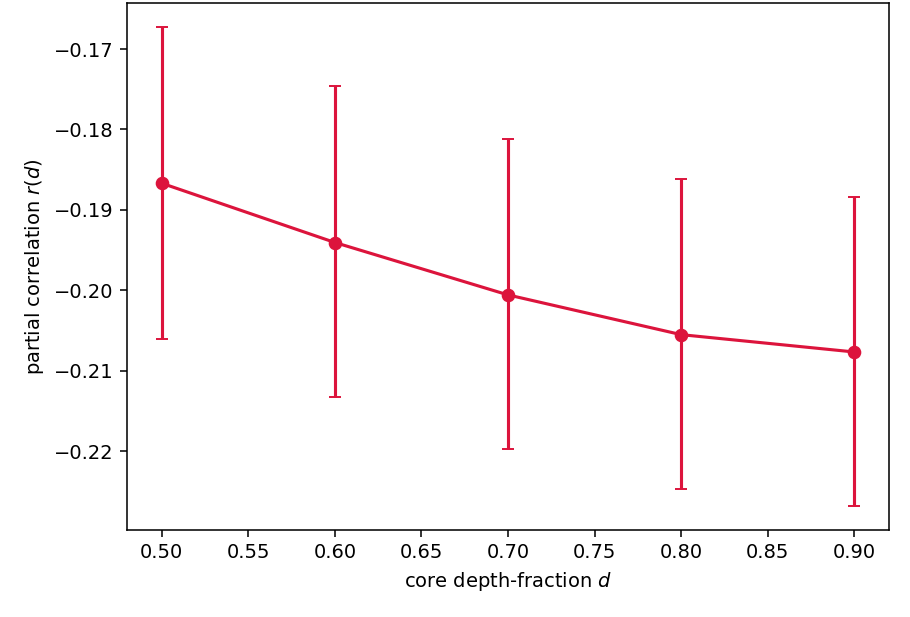
\includegraphics[width=0.6\textwidth]{depth_sensitivity.png}
\caption{Partial correlation (PC1 flux regressor) between interior and exterior state as a function of core depth, using the local-distance-transform definition described in the text and the merge-based segmentation of \S\ref{sec:individuation}, on \nn{\DepthFrames} frames of the $1024\times1024$ single-trajectory run ($N=\nn{\DepthN}$ organism-instances per point, error bars are 95\% CI). The partial correlation moves from $\rr{4}{\DepthROne}$ at $d=0.5$ to $\rr{4}{\DepthRFive}$ at $d=0.9$. This robustness check supports the interior-state definition used throughout the main text's \S\ref{sec:blanket} (main text \S\ref{sec:individuation}).}
\label{fig:S_depth_sensitivity}
\end{figure}

\subsection{The Merge Correction: Procedure, Convergence Check, and Figure}
\label{sec:S_merge_procedure}

Procedure (\texttt{merge\_overlapping\_organisms} in \texttt{run\_ensemble\_merged.py}). After raw watershed segmentation, every pair of raw regions that shares a boundary (is adjacent on the periodic grid) is examined. Each region's equivalent radius is $\sqrt{\text{area}/\pi}$ and its centroid is a circular-mean (periodic-correct) centroid; a pair is fused whenever its edge-to-edge gap, centroid distance minus the sum of the two radii, is negative. Fusions are applied together with a union--find, the merged regions are relabelled, and the radii and centroids are recomputed; the loop repeats until a round fuses nothing, up to a cap of \texttt{MAX\_MERGE\_ROUNDS}$=6$. Only pairs that touch are tested. Each final organism records \texttt{merge\_size}, the number of raw regions fused into it.

Convergence check (\texttt{merge\_rounds\_check\_1024.py}). Applied to \nn{\MergeFrames} frames of the settled $1024\times1024$ trajectory, spaced 100 steps apart like the production sampling, the loop needed one fusing round on \nn{\MergeOneRound} of the \nn{\MergeFrames} frames; \nn{\MergeMoreThanOne} needed a second, and \nn{\MergeCapHits} reached the cap. After the final round, \nn{\MergeTouchingLeft} of the \nn{\MergeOrganisms} organisms overlapped another organism's equivalent-radius circle, whether touching or not, so the restriction to touching pairs leaves no overlapping pair behind. The script runs a traced copy of the production loop and verifies on every frame that it returns the same labels, organism count and \texttt{merge\_size} as the production function.

Figure~\ref{fig:merge_correction}. The two panels are drawn by \texttt{make\_merge\_figure.py} from the settled checkpoint, using the production segmentation and merge functions directly, on a real pair whose circles overlap. The script lists the candidate pairs and their gaps and selects one with \texttt{--pick}; the pair shown is the second-largest overlap in the checkpoint frame (9 merged pairs in that frame). The pair is chosen for legibility, not at random.

\begin{figure}[!t]
\centering
\begin{minipage}[t]{0.42\textwidth}\centering
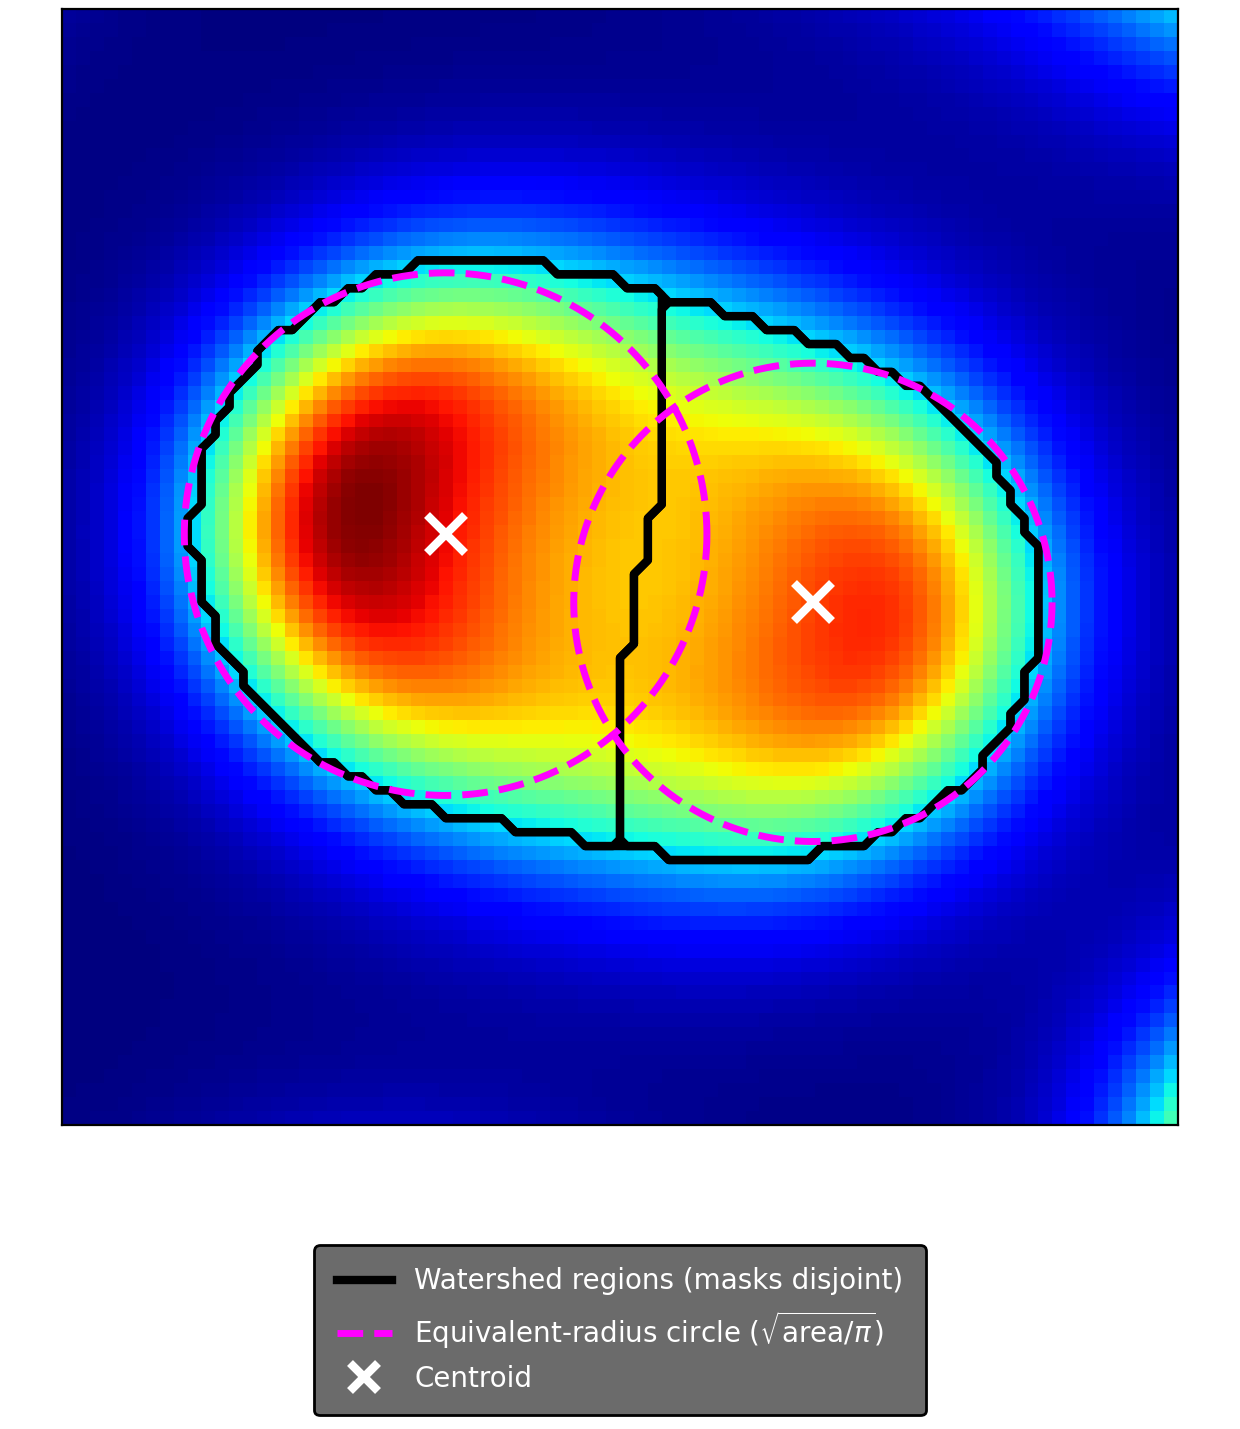
\includegraphics[width=\textwidth]{merge_before.png}\\[-2pt]{\small (a) Raw watershed}
\end{minipage}\hfill
\begin{minipage}[t]{0.42\textwidth}\centering
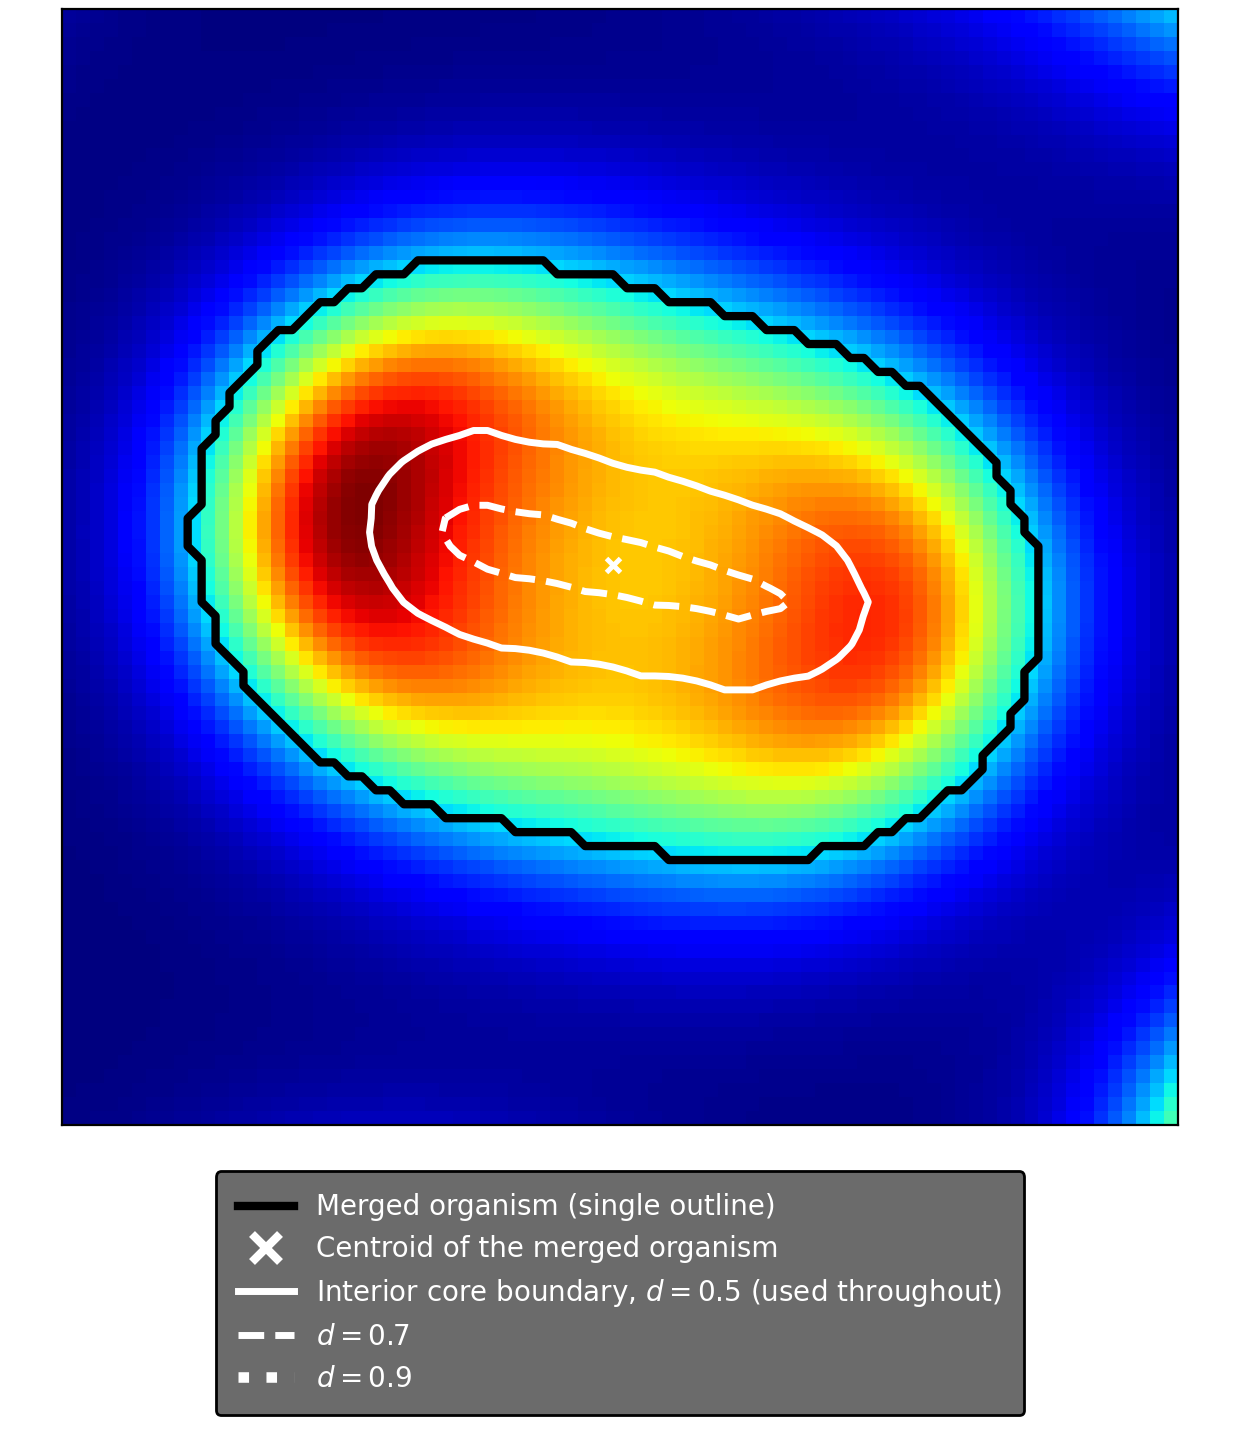
\includegraphics[width=\textwidth]{merge_after.png}\\[-2pt]{\small (b) After merge correction}
\end{minipage}
\caption{The merge correction on a real pair of watershed regions from the settled $1024\times1024$ trajectory (colours: activator field $v$). (a) Raw watershed splits one blob into two disjoint regions (black outlines; white $\times$, centroids). The dashed circles have each region's equivalent radius, $\sqrt{\text{area}/\pi}$; they overlap, since the centroid distance is less than the sum of the radii. (b) The pair is fused into one organism with a single outline and a single centroid ($\times$). The white contours bound the interior core for depth fractions $d=0.5$ (solid, used throughout), $0.7$ (dashed) and $0.9$ (dotted): a pixel belongs to the core if its distance from the nearest point outside the organism is at least $d$ times the organism's radius $\sqrt{\text{area}/\pi}$, so larger $d$ gives a smaller core nearer the centre. Both panels show the same window.}
\label{fig:merge_correction}
\end{figure}

\section{Supporting Checks for the Conditional-Independence Result (Main Text \S\ref{sec:conditional_independence})}
\label{sec:S_ci_support}

The main text's \S\ref{sec:conditional_independence} reports the paper's central result: a decisively nonzero partial correlation and nonlinear conditional mutual information between interior and exterior state after conditioning on blanket flux, both linearly and nonlinearly, in both a single trajectory and an independent ensemble. This section gives the full detail behind two supporting checks summarised briefly there: the five alternative-explanation checks (\S\ref{sec:alt_explanations}), and the non-watershed individuation robustness check (\S\ref{sec:levelset}).

\subsection{Alternative-Explanation Checks}
\label{sec:S_alt_explanations}

Before accepting the main text's \S\ref{sec:conditional_independence} result as a genuine blanket violation, we checked five alternative, less interesting explanations. First, that the effect might be an artefact of local crowding density rather than blanket leakage: adding local organism density (number of neighbours within 80 pixels) as an additional regressor on the single-trajectory dataset ($N=\nn{\TrajN}$) leaves the flux-conditioned partial correlation of the same sign and, if anything, slightly stronger ($r=\rr{3}{\AltCrowding}$ against $\rr{3}{\AltBaseline}$), ruling this out as an explanation. Second, that the effect might reflect an unbounded, whole-domain confound rather than a spatially local one: the main text's \S\ref{sec:corrlength} shows the coupling has real, bounded spatial structure (concentrated within about one organism radius), inconsistent with a simple diffuse confound.

Third, that life-cycle stage might drive the correlation: organisms early or late in their division cycle could differ systematically in both interior and exterior state for reasons unrelated to blanket leakage. Using the lineage-tracked age data of \S\ref{sec:falsestarts} (tracking merge-fused organisms; $N=\nn{\AgeN}$ measurements across $\nn{\AgeLineages}$ lineages, both completed and still-active, ages $\nn{\AgeMin}$--$\nn{\AgeMax}$ time units, median $\nn{\AgeMedian}$), the baseline partial correlation on this dataset (PC1 flux regressor, as throughout) is $r=\rr{3}{\AgeBaseline}$ (95\% CI $[\rr{3}{\AgeBaseLo},\rr{3}{\AgeBaseHi}]$, lineage-cluster bootstrap, resampling whole lineages rather than individual measurements to respect within-lineage autocorrelation), the same as the single-trajectory cross-sectional value. The lineage-tracked sample is a different, time-correlated sample of organisms (every fifth step, restricted to organisms the tracker follows), and we use it only for the comparisons within it. Adding organism age as a second covariate alongside blanket flux moves the estimate to $r=\rr{3}{\AgeWithAge}$ (95\% CI $[\rr{3}{\AgeWithLo},\rr{3}{\AgeWithHi}]$)---if anything strengthening rather than weakening the effect. Stratifying by age tercile shows that the partial correlation is weakest in the youngest tercile and much stronger in the other two ($r=\rr{3}{\AgeYoungR}$ young, $95\%$ CI $[\rr{3}{\AgeYoungLo},\rr{3}{\AgeYoungHi}]$; $r=\rr{3}{\AgeMidR}$ mid, CI $[\rr{3}{\AgeMidLo},\rr{3}{\AgeMidHi}]$; $r=\rr{3}{\AgeOldR}$ old, CI $[\rr{3}{\AgeOldLo},\rr{3}{\AgeOldHi}]$): every tercile's CI excludes zero, and the effect is present at all ages but roughly four times weaker in organisms younger than about $\nn{\AgeTercileEdge}$ time units. Read this way, the effect is not a fixed property present at full strength from the moment of division but one that strengthens over an organism's lifecycle. Either reading is inconsistent with life-cycle stage being a confound that explains away the reported violation.

Fourth, that the population-level result might be a mixture (ecological-correlation) artefact of pooling many different organisms together, rather than a genuine within-organism, moment-to-moment coupling: different lineages could simply sit at different average interior, exterior, and flux levels, generating an apparent population-wide dependence out of purely between-organism variation even if no single organism's own state ever really tracks its own flux fluctuations. A lineage-tracked dataset lets us test this directly, since it is longitudinal at the level of individual organism identity, unlike the cross-sectional datasets used elsewhere in this paper. We computed a lineage fixed-effects (``within'') partial correlation on the $N=\nn{\AgeN}$ lineage-tracker dataset used above: demeaning $I$, $E$ and the PC1 flux regressor separately \emph{within each lineage} before computing the partial correlation, so only how an organism's own state co-varies with its own flux fluctuations, relative to its own average, can contribute. This gives $r=\rr{3}{\LineageWithinR}$ (95\% CI $[\rr{3}{\LineageWithinLo},\rr{3}{\LineageWithinHi}]$, lineage-cluster bootstrap)---decisively nonzero and stronger than the pooled estimate above ($r=\rr{3}{\AgeBaseline}$). A complementary law-of-total-covariance decomposition of the flux-residualized $I$, $E$ into within-lineage and between-lineage components (grouped by organism identity) attributes all of the covariance to the within-lineage term ($\rr{0}{\LineageWithinPercent}\%$ within, $\rr{0}{\LineageBetweenPercent}\%$ between; 95\% CI on the within-lineage share $[\rr{0}{\LineageShareLo}\%,\rr{0}{\LineageShareHi}\%]$): the between-lineage term is slightly positive, so it works against the violation rather than producing it. The reported violation is therefore not a between-organism mixture effect masquerading as a population-level one but a within-organism, moment-to-moment coupling.

Fifth, that organism size and shape, or a frame-wide global driver (population count, mean substrate concentration, or segmentation threshold, all of which fluctuate together as the population grows and thins), might confound the result. On the single-trajectory dataset ($N=\nn{\TrajN}$), with each instance's equivalent-circle radius and shape eccentricity recorded alongside its own frame's population count, mean $u$, and Otsu($v$) threshold, the baseline flux-conditioned partial correlation is $r=\rr{3}{\AltBaseline}$. Frame-wide covariates barely matter: adding population, mean $u$ and threshold gives $r=\rr{3}{\AltFrameCovR}$ ($\nn{\AltFrameCovPercent}\%$ in magnitude), and frame fixed effects (demeaning within frame) give $r=\rr{3}{\AltFrameEffectsR}$. Organism size by itself is not a common cause of $I$ and $E$: radius correlates only $\rr{2}{\SizeRadiusI}$ with $I$ and $\rr{2}{\SizeRadiusE}$ with $E$, conditioning on radius alone leaves the marginal correlation almost unchanged ($\rr{3}{\SizeMarginalTwo}\to\rr{3}{\SizeRadiusOnlyTwo}$), and within five radius bins the marginal correlation stays between $\rr{2}{\SizeBinMargHi}$ and $\rr{2}{\SizeBinMargLo}$. Adding radius and eccentricity to the flux conditioning, however, reverses the sign of the partial correlation ($r=\rr{3}{\AltRadiusEccentricity}$; radius alone $\rr{3}{\SizeRadiusOnlyR}$, eccentricity alone $\rr{3}{\SizeEccOnlyR}$, area alone $\rr{3}{\SizeAreaOnlyR}$), and within radius bins the flux-conditioned partial correlation ranges from $\rr{2}{\SizeBinLo}$ to $\rr{2}{\SizeBinHi}$. We do not interpret this as size explaining the dependence. Radius is strongly collinear with the flux: it correlates $\rr{2}{\SizeRadiusFluxU}$ with $\Phi_u$ and $\rr{2}{\SizeRadiusPCOne}$ with the first principal component of the flux ($R^2=\rr{2}{\SizeRsqPCOneRadius}$), so once size is removed from the flux what remains is almost entirely a readout of the interior state (correlation with $I$ of $\rr{2}{\SizeResidI}$ in the full sample and $\rr{2}{\SizeBinResidHi}$ to $\rr{2}{\SizeBinResidLo}$ within radius bins, against $\rr{2}{\SizeIPCOne}$ before adjustment). Conditioning on that residual nearly conditions on $I$ itself, and the partial correlation of $I$ with $E$ given a near-deterministic function of $I$ is ill-conditioned and can take either sign. This is consistent with the collider-like behaviour of the flux covariates reported in the main text (the flux responds to both sides of the boundary), and it means that conditioning on flux after removing its size-driven component does not isolate a size confound. The honest summary is that the magnitude of the flux-conditioned residual correlation is sensitive to how much of the flux's non-$I$ variation is removed, which is why we report the nonlinear test of the main text's \S\ref{sec:ci_cmi} as the primary evidence and treat the flux-conditioned linear partial correlation as descriptive. A related instability affects the near-field $u$-shell covariates (seven shells out to 64 pixels): added individually they give partial correlations from $\rr{2}{\AltUShellMax}$ to $\rr{2}{\AltUShellMin}$, added jointly $\rr{2}{\AltUShellJoint}$, and the sign depends on the shell, so we draw no conclusion from them either.

These checks address the most obvious alternative explanations we identified; they do not exhaustively rule out every possible confound (boundary curvature or a shared-resource field are further candidates we have not separately tested), and we do not claim otherwise.

\subsection{Robustness to an Independent, Non-Watershed Individuation Method}
\label{sec:S_levelset}

Because watershed segmentation constructs organism boundaries relationally---the saddle geometry between touching or nearby basins is, by definition, jointly determined by neighbouring spots (\S\ref{sec:individuation})---one might worry that the conditional-independence violation reported in the main text's \S\ref{sec:conditional_independence} is itself an artefact of this individuation method, rather than a property of the underlying physical system. We tested this directly, individuating organisms by an entirely different method with no watershed, no basin competition, and no neighbour-dependence built into its construction: a fixed threshold on $v$ ($0.1356$, an empirically-measured plateau value of boundary $v$ for well-separated organisms) applied directly to the field, taking connected components of $\{v > 0.1356\}$ as candidate organisms. Components containing exactly one local maximum of $v$ (maxima found with the same marker spacing of 24 pixels as the watershed) are unambiguous single organisms; components containing zero or multiple maxima (noise, or organisms too close together for this simpler method to separate) cannot be individuated this way at all and are excluded from that construction. The check runs on $\nn{\LevelFrames}$ archived frames of the single trajectory (every fifth of the $\nn{\MasterFrames}$ frames; no new simulation), so it uses exactly the same fields as the watershed analysis. Of $\nn{\LevelComponents}$ components, $\nn{\LevelSingleMax}$ ($\rr{1}{\LevelSingleMaxPercent}\%$) have a single maximum and $\nn{\LevelZeroMax}$ ($\rr{1}{\LevelZeroMaxPercent}\%$) none, leaving the remainder multi-maximum; $N=\nn{\LevelSingleN}$ single-maximum organism-instances have finite values of all variables.

On these single-maximum instances, the partial correlation between interior and exterior state, controlling for blanket flux, is $r=\rr{3}{\LevelSingleR}$ (naive 95\% CI $[\rr{3}{\LevelSingleNaiveLo},\rr{3}{\LevelSingleNaiveHi}]$; marginal $r=\rr{3}{\LevelSingleMarginal}$)---larger in magnitude than the watershed-based result on the same frames ($r=\rr{3}{\AltBaseline}$, main text \S\ref{sec:conditional_independence}).\footnote{This partial correlation, and every other one reported in this subsection, is computed against a single flux regressor built from the leading principal component of standardized $(\Phi_u,\Phi_v)$, rather than the two raw flux variables jointly, because $\Phi_u$ and $\Phi_v$ are highly collinear ($r=\rr{2}{\FluxCollinearity}$) and the joint regression gives larger estimates that vary more between subsets (\S\ref{sec:S_pc1}, \S\ref{sec:S_isolated_followups}). For reference, the joint two-variable values here are $\rr{3}{\LevelSingleJoint}$ (single-maximum), $\rr{3}{\LevelRecoveredJoint}$ (recovered) and $\rr{3}{\LevelPooledJoint}$ (pooled); the pooled joint estimate changes sign, a sensitivity that the PC1 convention avoids (the joint design is numerically well conditioned once standardized; see \S\ref{sec:S_pc1}). Confidence intervals in this subsection are naive and ignore within-frame clustering.} Before treating that as convergent evidence, however, the exclusion criterion itself needs scrutiny: the excluded multi-maximum components are, by construction, exactly the touching or closely-spaced organism pairs a competitive-depletion account of crowding makes the strongest predictions about, so discarding them is a selection effect, not a neutral filtering step. We checked this directly: within each excluded multi-maximum component, we ran a second, LOCAL watershed split using only that component's own local maxima as markers, recovering interior/exterior states for $\nn{\LevelRecoveredN}$ organism-instances that the single-maximum construction discards ($\rr{1}{\LevelRecoveredPercent}\%$ of the pooled sample). On these recovered organism-instances alone, the partial correlation is $r=\rr{3}{\LevelRecoveredR}$ (naive 95\% CI $[\rr{3}{\LevelRecoveredNaiveLo},\rr{3}{\LevelRecoveredNaiveHi}]$), and pooling them with the single-maximum organisms gives a full-population estimate of $r=\rr{3}{\LevelPooledR}$ (naive 95\% CI $[\rr{3}{\LevelPooledNaiveLo},\rr{3}{\LevelPooledNaiveHi}]$, $N=\nn{\LevelPooledN}$; marginal $r=\rr{3}{\LevelPooledMarginal}$).

This resolves the apparent discrepancy in part. The single-maximum subset's larger magnitude ($r=\rr{3}{\LevelSingleR}$) is a selection effect of excluding merged pairs, not evidence that this construction is a more sensitive detector. Once the excluded pairs are recovered, the level-set estimate ($r=\rr{3}{\LevelPooledR}$) has the same sign as, and is decisively nonzero like, the watershed estimate, but it is only about a third of its magnitude ($r=\rr{3}{\AltBaseline}$). We therefore take this check as showing that the conditional dependence does not depend on watershed segmentation for its existence, and not as showing that its magnitude is independent of the individuation method: it is not, and the pooled estimate relies on a local watershed split for $\rr{1}{\LevelRecoveredPercent}\%$ of its organisms, so it is not fully independent of watershed construction either. A result that had differed in sign would have counted against the reported violation; this one did not, but the quantitative disagreement is real and we report it as such.

\paragraph{Nonlinear test on the level-set organisms.} We also ran the nonlinear CMI of the main text on these organisms (\texttt{run\_levelset\_cmi.py}; Frenzel--Pompe $k_{\mathrm{NN}}=5$, all variables $z$-scored, flux $(\Phi_u,\Phi_v)$ as the conditioning set, local nearest-neighbour null with 100 trials, subsamples of at most $N=\nn{\CmiNSub}$):
\begin{center}\small
\begin{tabular}{lrcccc}
\hline
Group & $N$ & $\mathrm{MI}(I;E)$ & $\mathrm{CMI}(I;E\mid\text{flux})$ & Null mean (SD) & Excess\\
\hline
Single-maximum & \nn{\LevelCmiSingleN} & \rr{4}{\LevelCmiSingleMI} & \rr{4}{\LevelCmiSingleCMI} & \rr{4}{\LevelCmiSingleNullMean} (\rr{4}{\LevelCmiSingleNullSD}) & \rr{1}{\LevelCmiSingleSD} SD\\
Recovered pairs & \nn{\LevelCmiRecoveredN} & \rr{4}{\LevelCmiRecoveredMI} & \rr{4}{\LevelCmiRecoveredCMI} & \rr{4}{\LevelCmiRecoveredNullMean} (\rr{4}{\LevelCmiRecoveredNullSD}) & \rr{1}{\LevelCmiRecoveredSD} SD\\
Pooled & \nn{\LevelCmiPooledN} & \rr{4}{\LevelCmiPooledMI} & \rr{4}{\LevelCmiPooledCMI} & \rr{4}{\LevelCmiPooledNullMean} (\rr{4}{\LevelCmiPooledNullSD}) & \rr{1}{\LevelCmiPooledSD} SD\\
\hline
\end{tabular}
\end{center}
For the single-maximum and pooled samples, conditioning on flux \emph{raises} the dependence (ratio \rr{1}{\LevelCmiSingleRatio}--\rr{1}{\LevelCmiPooledRatio}), as for watershed organisms, and the excess is far outside the null. The recovered pairs behave differently: flux removes more than half of a small dependence, leaving \rr{3}{\LevelCmiRecoveredCMI} nats at \rr{1}{\LevelCmiRecoveredSD} null standard deviations. So for this subset the flux comes closer to screening, although it does not reach the null. The subset is small, its unconditioned dependence is itself weak, and its states come from a local watershed split, so we do not read it as a separate finding. The pooled linear partial correlation ($r=\rr{3}{\LevelPooledR}$) is much smaller than that of either group alone, and the pooled joint estimate changes sign. A likely reason is that the groups differ in mean flux and interior state, so a single pooled regression absorbs some of the between-group difference, but we have not tested this. The nonlinear pooled result is a more direct comparison with the watershed analysis than the linear one, since it does not depend on a single linear regressor.

\subsection{A Second Independent Ensemble (Main Text \S\ref{sec:ci_ensemble})}
\label{sec:S_ensemble2}

A second set of $\nn{\EnsTwoRealisations}$ realisations, with seeds disjoint from the primary ensemble and otherwise the same production methodology and solver, reproduces the primary result. Its pooled flux-conditioned (PC1) partial correlation is $r=\rr{4}{\EnsTwoPartial}$ ($N=\nn{\EnsTwoN}$), against $\rr{4}{\EnsOnePartial}$ for the primary ensemble ($N=\nn{\EnsOneN}$). A realisation-cluster bootstrap (resampling whole realisations, the correct unit of independence here) gives 95\% CIs of $[\rr{4}{\EnsTwoBootLo},\rr{4}{\EnsTwoBootHi}]$ and $[\rr{4}{\EnsOneBootLo},\rr{4}{\EnsOneBootHi}]$ respectively, modestly wider than the naive intervals, as expected. Computing the partial correlation separately for each realization gives a unimodal, roughly symmetric distribution around the pooled estimate: mean $\rr{4}{\EnsTwoRealMean}$, median $\rr{4}{\EnsTwoRealMedian}$ and interquartile range $[\rr{4}{\EnsTwoRealQOne},\rr{4}{\EnsTwoRealQThree}]$ for the second set, and mean $\rr{4}{\EnsOneRealMean}$, median $\rr{4}{\EnsOneRealMedian}$ and interquartile range $[\rr{4}{\EnsOneRealQOne},\rr{4}{\EnsOneRealQThree}]$ for the primary ensemble. $\nn{\EnsTwoSameSign}$ of $\nn{\EnsTwoRealisations}$ realizations of the second set share the pooled estimate's sign, and $\nn{\EnsOneSameSign}$ of $\nn{\EnsOneRealisations}$ do for the primary ensemble. Individual realizations range more widely than the pooled confidence interval suggests because each carries far fewer organism-instances than the pooled set.

\paragraph{A third ensemble with longer burn-in and sample spacing.} In the first two ensembles the three samples of a realisation were taken $\nn{\SpacingOne}$ steps apart after the $\nn{\BurninOne}$-step burn-in. We also ran a third ensemble, with new seeds ($\nn{\SeedThree}+i$), the same burn-in of $\nn{\BurninThree}$ steps and $\nn{\SpacingThree}$ steps between samples. It has $\nn{\EnsThreeRealisations}$ realisations ($N=\nn{\EnsThreeN}$ organism-instances; \texttt{run\_ensemble\_merged.py --burn-in-steps \BurninThree\ --sample-spacing-steps \SpacingThree}, analysed with \texttt{analyze\_ensemble\_pc1.py}). The pooled PC1 partial correlation is $r=\rr{4}{\EnsThreePartial}$ (realisation-cluster bootstrap 95\% CI $[\rr{4}{\EnsThreeBootLo},\rr{4}{\EnsThreeBootHi}]$), against $\rr{4}{\EnsOnePartial}$ and $\rr{4}{\EnsTwoPartial}$ for the first two. The per-realization distribution is similar (mean $\rr{4}{\EnsThreeRealMean}$, SD $\rr{3}{\EnsThreeRealSD}$, interquartile range $[\rr{3}{\EnsThreeRealQOne},\rr{3}{\EnsThreeRealQThree}]$ against $[\rr{3}{\EnsOneRealQOne},\rr{3}{\EnsOneRealQThree}]$ and $[\rr{3}{\EnsTwoRealQOne},\rr{3}{\EnsTwoRealQThree}]$), and $\nn{\EnsThreeSameSign}$ of $\nn{\EnsThreeRealisations}$ realizations share the pooled sign. The three pooled values differ by up to \rr{3}{\EnsSpread}. The third ensemble also has more organisms per realisation (mean \rr{1}{\EnsThreePerRealN} against \rr{1}{\EnsOnePerRealN} and \rr{1}{\EnsTwoPerRealN}; standard deviation \rr{1}{\EnsThreePerRealNSD} against \rr{1}{\EnsOnePerRealNSD} and \rr{1}{\EnsTwoPerRealNSD}). The joint two-flux value is \rr{3}{\PcThreeJoint}, against \rr{3}{\PcOneJoint} and \rr{3}{\PcTwoJoint} for the first two ensembles. The single-flux values for the third ensemble are \rr{3}{\PcThreeFluxU} ($\Phi_u$ alone) and \rr{3}{\PcThreeFluxV} ($\Phi_v$ alone). The joint value depends on the small direction orthogonal to PC1 (\S\ref{sec:S_pc1}), which is why the paper uses PC1 as the reference convention.

\section{The PC1 Flux Regressor (Main Text \S\ref{sec:ci_ensemble})}
\label{sec:S_pc1}

The linear partial correlations in the main text condition on a single flux regressor, the leading principal component (PC1) of the standardised flux pair $(\Phi_u,\Phi_v)$, plus an intercept. This section gives the details of that choice and what the alternative gives. Table~\ref{tab:pc1} lists, for the single trajectory and the three independent ensembles, how collinear the two fluxes are, how much of their variance PC1 carries, and the $I$--$E$ partial correlation under four conditioning choices (script \texttt{pc1\_details.py}).

\paragraph{Definition.} Index the organism-instances by $i=1,\dots,N$ (one organism at one archived frame; $N=\nn{\TrajN}$ for the single trajectory). Each instance has an interior state $I_i$, an exterior state $E_i$ and fluxes $\Phi_{u,i},\Phi_{v,i}$. The fluxes are standardised across all instances,
\begin{equation}
z_{u,i}=\frac{\Phi_{u,i}-\bar\Phi_u}{s_u},\qquad z_{v,i}=\frac{\Phi_{v,i}-\bar\Phi_v}{s_v},
\end{equation}
\begin{equation}
\bar\Phi_x=\frac1N\sum_{i=1}^{N}\Phi_{x,i},\qquad s_x^2=\frac1{N-1}\sum_{i=1}^{N}\bigl(\Phi_{x,i}-\bar\Phi_x\bigr)^2,\qquad x\in\{u,v\}.
\end{equation}
Their correlation matrix is $\begin{pmatrix}1&\rho\\ \rho&1\end{pmatrix}$ with $\rho=\frac1{N-1}\sum_{i}z_{u,i}z_{v,i}$. Its eigenvectors are $(1,\pm1)/\sqrt2$ with eigenvalues $1\pm\rho$. For $\rho<0$ (here $\rho=\rr{3}{\PcTrajRho}$) the leading one is $(1,-1)/\sqrt2$, so
\begin{equation}
P_i=\frac{z_{u,i}-z_{v,i}}{\sqrt2},\qquad \frac1{N-1}\sum_{i=1}^{N}P_i^2=1-\rho ,
\end{equation}
which carries the fraction $(1-\rho)/2$ of the total variance (\rr{1}{\PcTrajVar}\% here). The overall sign of $P_i$ is arbitrary and does not affect the partial correlation. The partial correlation of $I$ and $E$ given $P$ is
\begin{equation}
r(I,E\,|\,P)=\frac{\sum_{i=1}^{N}\hat\varepsilon^{\,I}_i\,\hat\varepsilon^{\,E}_i}{\sqrt{\sum_{i=1}^{N}(\hat\varepsilon^{\,I}_i)^2\,\sum_{i=1}^{N}(\hat\varepsilon^{\,E}_i)^2}}
=\frac{r_{IE}-r_{IP}\,r_{EP}}{\sqrt{(1-r_{IP}^2)(1-r_{EP}^2)}},
\end{equation}
where $\hat\varepsilon^{\,I}_i=I_i-\hat a_I-\hat b_IP_i$ and $\hat\varepsilon^{\,E}_i=E_i-\hat a_E-\hat b_EP_i$ are the residuals of least-squares regressions of $I$ and of $E$ on $[1,P]$ over all $N$ instances, and $r_{IE},r_{IP},r_{EP}$ are the ordinary correlations across instances. All sums run over instances, never over time within one organism.

\begin{table}[htbp]
\centering
\footnotesize

\setlength{\tabcolsep}{3.5pt}
\begin{tabular}{lrccccccc}
\toprule
Dataset & $N$ & $r(\Phi_u,\Phi_v)$ & PC1 var. & $\kappa$ raw / std. & PC1 & Joint & $\Phi_u$ only & $\Phi_v$ only \\
\midrule
Single trajectory & \nn{\PcTrajN} & \rr{4}{\PcTrajRho} & $\rr{2}{\PcTrajVar}\%$ & \num{\PcTrajKappaRaw} / \rr{1}{\PcTrajKappaStd} & \rr{4}{\PcTrajPc} & \rr{4}{\PcTrajJoint} & \rr{4}{\PcTrajFluxU} & \rr{4}{\PcTrajFluxV} \\
Ensemble, seed \SeedOne & \nn{\PcOneN} & \rr{4}{\PcOneRho} & $\rr{2}{\PcOneVar}\%$ & \num{\PcOneKappaRaw} / \rr{1}{\PcOneKappaStd} & \rr{4}{\PcOnePc} & \rr{4}{\PcOneJoint} & \rr{4}{\PcOneFluxU} & \rr{4}{\PcOneFluxV} \\
Ensemble, seed \SeedTwo & \nn{\PcTwoN} & \rr{4}{\PcTwoRho} & $\rr{2}{\PcTwoVar}\%$ & \num{\PcTwoKappaRaw} / \rr{1}{\PcTwoKappaStd} & \rr{4}{\PcTwoPc} & \rr{4}{\PcTwoJoint} & \rr{4}{\PcTwoFluxU} & \rr{4}{\PcTwoFluxV} \\
Ensemble, seed \SeedThree & \nn{\PcThreeN} & \rr{4}{\PcThreeRho} & $\rr{2}{\PcThreeVar}\%$ & \num{\PcThreeKappaRaw} / \rr{1}{\PcThreeKappaStd} & \rr{4}{\PcThreePc} & \rr{4}{\PcThreeJoint} & \rr{4}{\PcThreeFluxU} & \rr{4}{\PcThreeFluxV} \\
\bottomrule
\end{tabular}
\caption{The two fluxes and the choice of flux regressor. $\kappa$ is the condition number of the joint-regression design matrix $[1,\Phi_u,\Phi_v]$, in raw flux units and after standardising the fluxes. The last four columns are the $I$--$E$ partial correlation conditioning on PC1, on both fluxes jointly, on $\Phi_u$ alone and on $\Phi_v$ alone.}
\label{tab:pc1}
\end{table}

$\Phi_u$ and $\Phi_v$ are almost perfectly anticorrelated, as the reaction's stoichiometry makes them (a molecule of $u$ consumed produces one of $v$), and PC1 carries $\rr{1}{\PcVarMin}$--$\rr{1}{\PcVarMax}\%$ of their joint variance. The large raw-unit condition number of the joint design matrix mostly reflects the scale of the fluxes ($\sim10^{-5}$) against the intercept; once the fluxes are standardised it is only $\nn{\PcKappaStdMin}$--$\nn{\PcKappaStdMax}$. The joint regression is therefore numerically well determined, and a ridge penalty of any strength from $0$ to $100$ leaves it unchanged (\S\ref{sec:S_isolated_followups}). It is not an artefact of rounding.

What the joint regression does give is a larger partial correlation ($\rr{2}{\PcJointAbsMin}$ to $\rr{2}{\PcJointAbsMax}$) than PC1 ($\rr{2}{\PcPcAbsMin}$ to $\rr{2}{\PcPcAbsMax}$), and larger than either single flux ($\rr{2}{\PcSingleAbsMin}$ to $\rr{2}{\PcSingleAbsMax}$). The joint value lies outside the range spanned by the two single-flux values in all four datasets, which is why we use PC1 as the reference convention. The two-variable fit uses the small direction orthogonal to PC1 (under $1\%$ of the flux variance), and that direction is correlated with $I$ and $E$ individually. Conditioning on it raises, rather than lowers, the apparent $I$--$E$ dependence (for the single trajectory, a screened fraction of $\rr{0}{\PcTrajJointScreened}\%$), the signature of conditioning on a variable that is a joint effect of both sides (the collider structure discussed in the main text's \S\ref{sec:blanket_formulation}). We report PC1 as the headline because it is the smaller of the estimates, so the conclusion that dependence survives conditioning does not rest on the larger one. We have not shown which of the two is the right description of the blanket; both give a clearly nonzero partial correlation.

\section{Periodic-Safe Distance Transform for the Spatial-Structure Analysis (Main Text \S\ref{sec:corrlength})}
\label{sec:S_corrlength}

The main text's \S\ref{sec:corrlength} characterises the conditional interior--exterior coupling's spatial extent by measuring $r(s)$, the partial correlation with the organism's exterior state redefined, shell by shell, as the mean $v$ in its own concentric shell at distance $s$ from its boundary, using a hybrid radial resolution (8-pixel steps out to 160 pixels, coarsening to 24-pixel steps out to 400 pixels, given $N=\nn{\TrajN}$ organism-instances under the merge-based segmentation of \S\ref{sec:individuation})---the same physical distances, in organism-radii, as the original $256\times256$ analysis.

Each organism's distance transform is computed on a local, modulo-indexed crop 920 pixels on a side (460-pixel half-width) centred on its own centroid, not a whole-domain, edge-padded array; this is what the main text's ``periodic-safe'' refers to. On the $1024\times1024$, $L=2.5$ domain used throughout ($\sim$20-pixel organism radius, so a domain $\sim$51 radii wide), the crop's 460-pixel half-width covers the full 400-pixel shell schedule plus organism extent with a 52-pixel margin, while remaining strictly smaller than the 512-pixel half-domain. The same organism's own periodic image, offset by a full domain width ($\pm$1024 pixels), therefore never falls inside the crop, and no shell (out to 400 pixels, 19--20 organism radii) can wrap onto it; a genuine neighbour's periodic image could in principle enter the crop only if that neighbour were within $512-460=52$ pixels of the domain's own periodic seam relative to the focal organism, a configuration the crop-based construction handles correctly by construction (direct modulo indexing of the true, singly-wrapped field) rather than by whole-image edge padding.

\subsection{Implementation of the Three-Variable Data Collection (\S\ref{sec:threevar_numerics})}
\label{sec:S_threevar_impl}

The individuation functions described above (\texttt{organism\_\allowbreak interior\_\allowbreak exterior\_\allowbreak states\_\allowbreak adaptive\_\allowbreak fast}, \texttt{organism\_\allowbreak shell\_\allowbreak profile\_\allowbreak field\_\allowbreak fast}) work on a crop around each organism with modulo-indexed coordinates, so that a crop crossing the periodic boundary wraps the domain exactly once. All results reported here use these functions. The three-variable data-collection script (\texttt{run\_3var\_shell\_data.py}) uses the merge-based individuation at marker spacing 24 (\S\ref{sec:threevar_blanket}). The plain Gray--Scott baseline is the merge-based correlation-length curve of main text \S\ref{sec:corrlength}.

\section{The Richer-Blanket Screening Curve: Full Construction and Discussion (Main Text \S\ref{sec:richer_blanket})}
\label{sec:S_richer_blanket}

We used the shell-profile data of the main text's \S\ref{sec:corrlength} to build a richer candidate blanket for testing whether the conditional-independence violation is an artefact of flux's low dimensionality: rather than the two flux scalars alone, we additionally condition on the organism's own $v$-value in each of $\nn{\ScreenNear}$ concentric exterior shells spanning its near-field oscillatory structure (out to $\rr{1}{\ScreenMidHi}$ organism radii, with mid-radii from \rr{2}{\ScreenMidLo} to \rr{2}{\ScreenMidHi} radii measured from the boundary, $R=\rr{1}{\ScreenRadiusPx}$ pixels)---an 18-dimensional conditioning set, in place of the original two scalars. We then ask whether this richer blanket screens off the organism's interior state from its own \emph{far-field} exterior (the mean $v$-value over $\nn{\ScreenFarShells}$ shells at \rr{1}{\ScreenFarLo}--\rr{1}{\ScreenFarHi} organism radii, the regime characterised in the main text's \S\ref{sec:corrlength} as small but persistent). All figures use the single-trajectory dataset ($N=\nn{\TrajN}$) and the PC1 flux convention.

Rather than testing only the flux-alone and full-enrichment endpoints, we constructed a screening curve: $r(n)$, the same partial-correlation construction repeated with the blanket expanded to include the first $n$ near-field shells alongside the flux, evaluated at every enrichment level from $n=0$ up to the full 16-shell profile, one additional shell at a time (Figure~\ref{fig:screening_curve}). With flux alone the partial correlation is $r=\rr{3}{\ScreenRZero}$. It is not a decay towards zero: adding the first shell moves it to $\rr{3}{\ScreenROne}$, the second to $\rr{3}{\ScreenRTwo}$, the third to $\rr{3}{\ScreenRThree}$, after which it plateaus (e.g.\ $\rr{3}{\ScreenRFive}$ at $n=5$, $\rr{3}{\ScreenRAll}$ at $n=\nn{\ScreenNear}$). The curve therefore does not show screening. Its sign reversal should not be read as evidence of anything about the blanket either: the innermost exterior shells are strongly collinear with the flux and with $I$ itself, and, as with the radius and $u$-shell covariates of \S\ref{sec:S_alt_explanations}, adding strongly collinear covariates to a partial correlation makes the adjusted value ill-conditioned.

\begin{figure}[htbp]
\centering
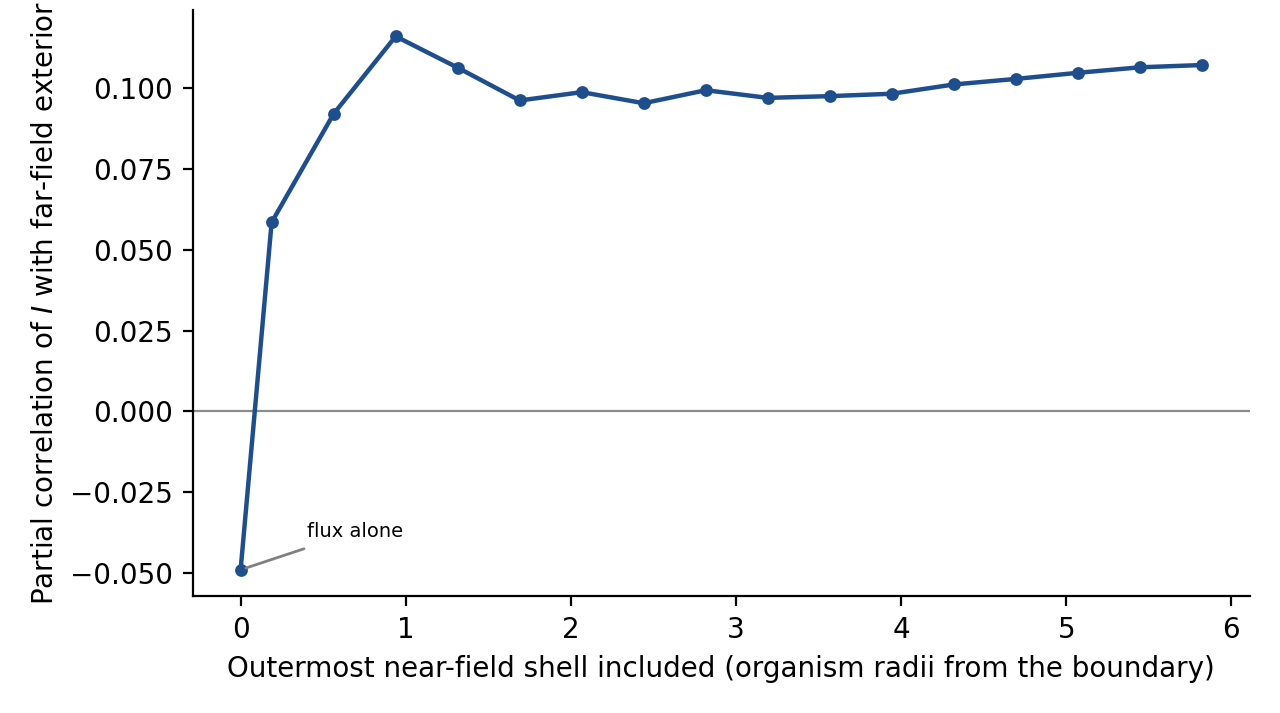
\includegraphics[width=0.8\textwidth]{screening_curve.png}
\caption{Screening curve: partial correlation between interior and far-field exterior state, as a function of how much near-field boundary information is included in the conditioning set (0 to $\nn{\ScreenNear}$ shells, out to \rr{1}{\ScreenMidHi} organism radii; $N=\nn{\TrajN}$). Adding the first shells reverses the sign of the partial correlation, which then plateaus near $+0.10$ from the fourth shell onward.}
\label{fig:screening_curve}
\end{figure}

This does not, and cannot, rule out that some other, untested enrichment of the blanket would succeed where this one did not; no finite test can establish that no such representation exists, and the ill-conditioning described above limits how much weight this linear check can carry in either direction. The case against a flux-independent blanket rests instead on the nonlinear test of the main text's \S\ref{sec:ci_cmi} and on the collider analysis of \S\ref{sec:S_collider_test}: a properly-scaled nonlinear conditional mutual information check finds that flux conditioning \emph{increases} the apparent nonlinear dependence relative to unconditioned in the full population, while conditioning on the boundary's own concentration state instead screens about $\rr{0}{\PooledBoundaryScreened}\%$ of it. That leaves most of the nonlinear conditional coupling unexplained by boundary-defined variables; it is removed only by a thick band of the surrounding field (\S\ref{sec:S_band}).

\section{Blanket-Thickness Sweep (Main Text \S\ref{sec:richer_blanket})}
\label{sec:S_band}

The substrate test of \S\ref{sec:S_u_enriched} conditions on $u$-shells that overlap the exterior ring over which $E$ is averaged, so it cannot tell a blanket from a proxy for $E$. This sweep removes the overlap: it asks how thick a band of the surrounding field must be to screen the interior from the field just beyond it. Its specification was fixed before any result was seen.

\paragraph{Design.} For a band of width $w\in\{0,8,16,24,40,64,96\}$ px beyond the organism's mask, the conditioning set is $Z_w=(\Phi_u,\Phi_v)$ plus up to three area-weighted mean-$v$ summaries of the band and up to three mean-$u$ summaries (the band is cut into thirds on the available shell edges; $u$ shells exist only to 64 px, only shells wholly inside the band are used, so $u$ summaries are absent for $w<12$). The exterior variable is the area-weighted mean $v$ over the 24-px shell immediately beyond the band, $E_w=\bar v[w,w+24]$, so nothing in $Z_w$ overlaps it. At $w=0$ the blanket is flux alone and $E_0$ is the shell-based 0--24 px mean (which differs slightly from the distance-transform ring $E$ used elsewhere). The statistic, $z$-scoring, nulls (30-group and local nearest-neighbour; 100 trials each), subsets, and $N=\nn{\CmiNSub}$ subsample are those of \S\ref{sec:S_u_enriched}. Controls at every width, with the same dimension as the real $Z_w$: \emph{noise}, in which the band columns are independently permuted (this approximates the dependence that remains given flux alone at that distance, with the same dimension penalty); and \emph{$E$-copy}, flux plus a noisy copy of $E_w$ with the $R^2$ to $E_w$ that the real band achieves, padded to the same dimension.

\paragraph{Result.} Table~\ref{tab:S_band} and Figure~\ref{fig:S_band} give the results, as means over three independent subsamples. With flux alone the CMI is \rr{3}{\BandOrgZero} nats. A band of 8 px leaves \rr{3}{\BandOrgEight} and 16 px leaves \rr{3}{\BandOrgSixteen} nats. From $w=24$ px, about one organism radius, the CMI is at most \rr{3}{\BandMaxThick} nats in every subsample (under $5\%$ of the flux-only value) and at most \rr{1}{\BandMaxThickSD} null SDs above its null, and it stays at that level at $w=40$, 64 and 96 px. The noise control stays near \rr{2}{\BandNoiseThick} nats at $w=24$--40, so the screening is due to the information in the band and is not a dimension effect. The residual of a few thousandths of a nat at $w=40$ is small but not exactly zero. The $E$-copy control screens as well as the real band. In a spatially continuous field this is expected: a band predicts the adjacent shell, and that is how screening by a thick band works.

\paragraph{What this establishes.} The conditional dependence between interior and exterior is concentrated within about one organism radius of the boundary, and a band of the surrounding field that thick screens the interior from the field beyond it, to within a few null SDs and under 0.01 nats, for these summaries. The paper's own exterior ring (0--24 px) lies entirely inside that band, which is why the flux-based test shows dependence. This is what any field with short-range coupling would give, so it does not indicate inference, and it does not show that the full Markov blanket condition holds (the band is summarised by six means, and the three subsamples come from one trajectory). The thin, boundary-defined blanket of the main text still fails.

\paragraph{Placebo disks.} To test whether the screening is specific to organisms, the same sweep was run on placebo disks (\texttt{run\_random\_disks.py}). For every third archived frame of the master trajectory, each organism is matched by a disk of the same equivalent radius, centred at a random position where the disk touches no organism and no other disk. For each disk the interior state, fluxes and shell profiles are measured with the same functions as for organisms. This gives $\nn{\DiskN}$ disks from $\nn{\DiskFrames}$ frames (mean radius \rr{1}{\DiskRadius} px against \rr{1}{\OrgRadiusMean} px for organisms). The specification of the sweep is unchanged, but the disks use one $N=\nn{\CmiNSub}$ subsample where the organisms use three (Table~\ref{tab:S_band_disks}). With flux alone the CMI is \rr{3}{\BandDiskZero} nats (\rr{1}{\BandDiskZeroSD} null SDs). A band of 8 px leaves \rr{3}{\BandDiskEight} nats (\rr{1}{\BandDiskEightSD} SDs), and from 16 px the CMI is at or below zero and no more than \rr{3}{\BandDiskExcess} nats above its null (\rr{1}{\BandDiskSDMax} SDs at most). The noise control, with the band information removed, is higher at every width up to 40 px. Disks are therefore screened by a band at least as thin as organisms are, and faster: at $w=8$ the organisms' dependence (\rr{3}{\BandOrgEight} nats) is about \rr{0}{\BandOrgOverDiskEight} times the disks'. We did not test why. The result shows that screening by a band of field is a property of the field and not of being an organism.

\begin{table}[htbp]
\centering
\footnotesize
\begin{tabular}{rrcccc}
\toprule
$w$ (px) & dim. & real & excess over null (cluster) & SD & noise \\
\midrule
0 & 2 & \rr{4}{\BandDiskZero} & \rr{4}{\BandDiskExcessZero} & \rr{1}{\BandDiskSDZero} & --- \\
8 & 4 & \rr{4}{\BandDiskEight} & \rr{4}{\BandDiskExcessEight} & \rr{1}{\BandDiskSDEight} & \rr{4}{\BandDiskNoiseEight} \\
16 & 6 & \rr{4}{\BandDiskSixteen} & \rr{4}{\BandDiskExcessSixteen} & \rr{1}{\BandDiskSDSixteen} & \rr{4}{\BandDiskNoiseSixteen} \\
24 & 8 & \rr{4}{\BandDiskTwentyFour} & \rr{4}{\BandDiskExcessTwentyFour} & \rr{1}{\BandDiskSDTwentyFour} & \rr{4}{\BandDiskNoiseTwentyFour} \\
40 & 8 & \rr{4}{\BandDiskForty} & \rr{4}{\BandDiskExcessForty} & \rr{1}{\BandDiskSDForty} & \rr{4}{\BandDiskNoiseForty} \\
64 & 8 & \rr{4}{\BandDiskSixtyFour} & \rr{4}{\BandDiskExcessSixtyFour} & \rr{1}{\BandDiskSDSixtyFour} & \rr{4}{\BandDiskNoiseSixtyFour} \\
96 & 8 & \rr{4}{\BandDiskNinetySix} & \rr{4}{\BandDiskExcessNinetySix} & \rr{1}{\BandDiskSDNinetySix} & \rr{4}{\BandDiskNoiseNinetySix} \\
\bottomrule
\end{tabular}
\caption{Blanket-thickness sweep on placebo disks (one $N=\nn{\CmiNSub}$ subsample of $\nn{\DiskN}$ disks, 100 null trials). CMI in nats, observed value and excess over the 30-group null mean in null SDs; the local nearest-neighbour null gives the same picture (\rr{1}{\BandDiskLocalSDZero} SDs at $w=0$, \rr{1}{\BandDiskLocalSDEight} at $w=8$, at most \rr{1}{\BandDiskLocalMaxAbs} in magnitude from $w=16$). Noise: band information removed.}
\label{tab:S_band_disks}
\end{table}

\begin{table}[htbp]
\centering
\footnotesize
\setlength{\tabcolsep}{3pt}

\begin{tabular}{rrrcrrr}
    \toprule
    $w$ (px) & dim. & real & [range] & max SD & noise & copy \\
    \midrule
    0 & 2 & \rr{3}{\BandOrgZero} & [\rr{3}{\BandOrgLoZero}, \rr{3}{\BandOrgHiZero}] & \rr{1}{\BandOrgMaxSDZero} & --- & --- \\
    8 & 4 & \rr{3}{\BandOrgEight} & [\rr{3}{\BandOrgLoEight}, \rr{3}{\BandOrgHiEight}] & \rr{1}{\BandOrgMaxSDEight} & \rr{3}{\BandOrgNoiseEight} & \rr{3}{\BandOrgCopyEight} \\
    16 & 6 & \rr{3}{\BandOrgSixteen} & [\rr{3}{\BandOrgLoSixteen}, \rr{3}{\BandOrgHiSixteen}] & \rr{1}{\BandOrgMaxSDSixteen} & \rr{3}{\BandOrgNoiseSixteen} & \rr{3}{\BandOrgCopySixteen} \\
    24 & 8 & \rr{3}{\BandOrgTwentyFour} & [\rr{3}{\BandOrgLoTwentyFour}, \rr{3}{\BandOrgHiTwentyFour}] & \rr{1}{\BandOrgMaxSDTwentyFour} & \rr{3}{\BandOrgNoiseTwentyFour} & \rr{3}{\BandOrgCopyTwentyFour} \\
    40 & 8 & \rr{3}{\BandOrgForty} & [\rr{3}{\BandOrgLoForty}, \rr{3}{\BandOrgHiForty}] & \rr{1}{\BandOrgMaxSDForty} & \rr{3}{\BandOrgNoiseForty} & \rr{3}{\BandOrgCopyForty} \\
    64 & 8 & \rr{3}{\BandOrgSixtyFour} & [\rr{3}{\BandOrgLoSixtyFour}, \rr{3}{\BandOrgHiSixtyFour}] & \rr{1}{\BandOrgMaxSDSixtyFour} & \rr{3}{\BandOrgNoiseSixtyFour} & \rr{3}{\BandOrgCopySixtyFour} \\
    96 & 8 & \rr{3}{\BandOrgNinetySix} & [\rr{3}{\BandOrgLoNinetySix}, \rr{3}{\BandOrgHiNinetySix}] & \rr{1}{\BandOrgMaxSDNinetySix} & \rr{3}{\BandOrgNoiseNinetySix} & \rr{3}{\BandOrgCopyNinetySix} \\
    \bottomrule
    \end{tabular}
\caption{Blanket-thickness sweep: means over three independent $N=\nn{\CmiNSub}$ subsamples (seeds 0, 1, 2), 100 null trials each. CMI $I(I;E_w\mid Z_w)$ in nats. ``Real'' is the CMI with the real band, with its range over the three subsamples; ``max SD'' is the largest distance of the observed value above the cluster-null mean, in null SDs, over the three subsamples. Noise: band information removed. Copy: noisy copy of $E_w$ with the real band's $R^2$. Dim.\ is the dimension of $Z_w$.}
\label{tab:S_band}
\end{table}

\begin{figure}[htbp]
\centering
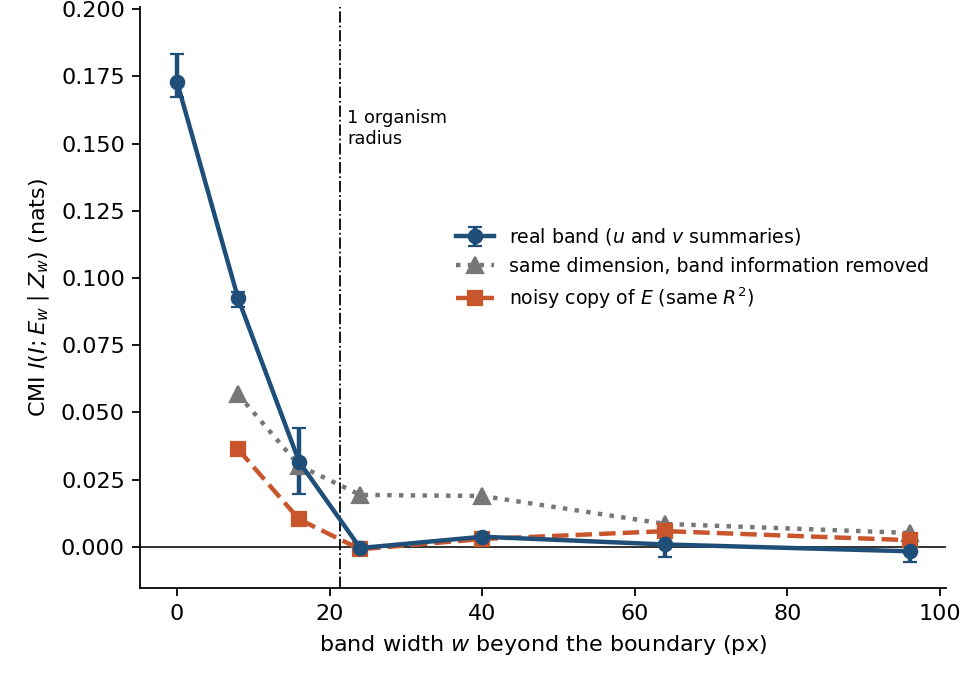
\includegraphics[width=0.7\textwidth]{band_sweep_cmi.png}
\caption{CMI between the interior and the 24-px shell beyond a band of width $w$, conditioning on flux and summaries of the band. The dashed vertical line marks one organism radius. The dependence is removed by a band about one radius thick. The noise curve (band information removed) shows what remains without the band's information. Points are means over three subsamples; bars show the range for the real band.}
\label{fig:S_band}
\end{figure}

\section{Substrate-Enriched Blanket Test (Main Text \S\ref{sec:richer_blanket})}
\label{sec:S_u_enriched}

The richer-blanket check of \S\ref{sec:S_richer_blanket} enriched the blanket with the organism's own $v$ and was linear. A referee-style objection is that the shared substrate $u$, which the reaction couples directly to $v$, is the more natural candidate for carrying the influence of neighbouring spots, and that the test should be nonlinear. We therefore ran the following test, with its specification fixed before any result was seen (no search over conditioning variables).

\paragraph{Design.} The conditioning set is $Z_n=(\Phi_u,\Phi_v)$ plus the first $n$ of seven mean-$u$ shells beyond the organism boundary (0--6, 6--12, 12--18, 18--24, 24--36, 36--48, 48--64 px), for $n\in\{0,1,2,3,5,7\}$. The statistic is the Frenzel--Pompe nearest-neighbour conditional mutual information $I(I;E\mid Z_n)$ ($k_{\mathrm{NN}}=5$) with every variable, including $I$ and $E$, $z$-scored before estimation. Two nulls are used, both preserving $p(E\mid Z_n)$ approximately: the 30-group null of the main text, which shuffles $E$ within each of $30$ $k$-means groups of similar $Z_n$, and a local null that swaps $E$ only among each point's ten nearest neighbours in $Z_n$ in the style of \citet{Runge2018}. Each uses 100 trials. The data are the single-trajectory master dataset ($N=\nn{\TrajN}$), with the same random $N=\nn{\CmiNSub}$ subsample for every conditioning set so that levels are directly comparable. Here $E$ is the exterior-ring mean $v$ (0--24 px) used throughout the main text.

\paragraph{Controls.} Adding dimensions lowers a nearest-neighbour CMI estimate even when the added variables carry no information, so each real-$u$ condition is paired with (i) \emph{noise columns}: flux plus 3 or 7 independently permuted $u$-shell columns (same marginals, no information); and (ii) an \emph{$E$-copy}: flux plus a copy of $E$ with independent Gaussian noise added so that its squared correlation with $E$ equals the $R^2$ with which the real $u$-shells predict $E$, padded with noise columns to the same dimension.

\paragraph{Result.} Table~\ref{tab:S_u_enriched} and Figure~\ref{fig:S_u_enriched} give the results. With flux alone the CMI is \rr{3}{\UEnrObsZero} nats (\rr{1}{\UEnrSDZero} cluster-null SDs, \rr{1}{\UEnrFluxLocalSD} local-null SDs). It falls steadily as $u$-shells are added, to \rr{3}{\UEnrObsThree} nats at $n=3$ and \rr{3}{\UEnrObsSeven} nats at $n=7$, where it is within about two null SDs of zero. Pure-noise columns of the same dimension reduce it only to \rr{3}{\UEnrNoiseObsThree} ($n=3$) and \rr{3}{\UEnrNoiseObsSeven} ($n=7$), so the reduction is not a dimension artefact.

The reduction does not, however, show that substrate shells form a blanket. Flux plus three $u$-shells predict $E$ linearly with $R^2=\rr{2}{\UEnrRsqEThreeFrac}$ (and seven shells, $R^2=\rr{2}{\UEnrRsqESevenFrac}$), against $R^2=\rr{2}{\UEnrRsqEZero}$ for flux alone: the shells lie inside the ring over which $E$ is averaged, and the reaction ties local $u$ to local $v$. They therefore carry most of $E$'s own value, and conditioning on a near-copy of $E$ removes the dependence between $I$ and $E$ almost regardless of any physical mechanism. The $E$-copy control confirms this: with the same $R^2$ and dimension it reduces the CMI to \rr{3}{\UEnrCopyObsThree} nats ($n=3$) and \rr{3}{\UEnrCopyObsSeven} nats ($n=7$), compared with \rr{3}{\UEnrObsThree} and \rr{3}{\UEnrObsSeven} for the real shells. The real shells screen slightly better than an independent-noise copy, which is expected because their departure from $E$ is structured rather than independent. The shell adjacent to the boundary (0--6 px, $n=1$) leaves \rr{3}{\UEnrObsOne} nats (\rr{0}{\UEnrOnePercent}\% of the flux-only value, still \rr{0}{\UEnrSDOne} null SDs); the screening appears only as the shells extend into $E$'s own territory.

\paragraph{Far-field exterior.} To avoid the overlap, we repeated the test with $E$ replaced by the mean $v$ over 184--400 px (9.2--18.2 radii), which does not overlap the $u$-shells. Here flux alone already leaves little to screen: \rr{3}{\UFarObsZero} nats (\rr{1}{\UFarSDZero} null SDs), consistent with the short-range coupling of the main text's \S\ref{sec:corrlength}. Every enriched condition is within about two null SDs of zero, as are the noise controls, so this version cannot discriminate between hypotheses. The coupling that violates the blanket condition is local, and the part of the exterior that the substrate shells can see is the part that overlaps $E$.

\paragraph{What this establishes.} Near-boundary substrate information can screen the interior from the near-field exterior, but the test cannot distinguish a genuine blanket from conditioning on a proxy for the exterior variable itself, and the far-field test has no dependence to screen. We therefore do not count it as evidence that the blanket condition is satisfied. A blanket variable that is nearly a function of the exterior state is, by construction, no longer separate from it. This leaves the conclusion about flux unchanged. The blanket-thickness sweep of \S\ref{sec:S_band} avoids the overlap by placing $E$ beyond the band. The number of null trials (100) and the single subsample limit the precision of the null-SD figures; the observed CMI values are stable to about $\pm0.005$ nats across subsamples in a pilot with $N=1500$.

\begin{table}[htbp]
\centering
\small

\begin{tabular}{llrrr}
\toprule
 & Conditioning set & dim. & CMI & excess (SD) \\
\midrule
 & flux only & 2 & \rr{3}{\UEnrObsZero} & \rr{3}{\UEnrExcZero} (\rr{1}{\UEnrSDZero}) \\
 & + 1 $u$-shell & 3 & \rr{3}{\UEnrObsOne} & \rr{3}{\UEnrExcOne} (\rr{1}{\UEnrSDOne}) \\
 & + 2 $u$-shells & 4 & \rr{3}{\UEnrObsTwo} & \rr{3}{\UEnrExcTwo} (\rr{1}{\UEnrSDTwo}) \\
 & + 3 $u$-shells & 5 & \rr{3}{\UEnrObsThree} & \rr{3}{\UEnrExcThree} (\rr{1}{\UEnrSDThree}) \\
 & + 5 $u$-shells & 7 & \rr{3}{\UEnrObsFive} & \rr{3}{\UEnrExcFive} (\rr{1}{\UEnrSDFive}) \\
 & + 7 $u$-shells & 9 & \rr{3}{\UEnrObsSeven} & \rr{3}{\UEnrExcSeven} (\rr{1}{\UEnrSDSeven}) \\
\midrule
\multicolumn{2}{l}{\emph{Controls}} \\
 & + 3 noise columns & 5 & \rr{3}{\UEnrNoiseObsThree} & \rr{3}{\UEnrNoiseExcThree} (\rr{1}{\UEnrNoiseSDThree}) \\
 & + 7 noise columns & 9 & \rr{3}{\UEnrNoiseObsSeven} & \rr{3}{\UEnrNoiseExcSeven} (\rr{1}{\UEnrNoiseSDSeven}) \\
 & $E$-copy, $R^2=\rr{2}{\UEnrRsqEThreeFrac}$ & 5 & \rr{3}{\UEnrCopyObsThree} & \rr{3}{\UEnrCopyExcThree} (\rr{1}{\UEnrCopySDThree}) \\
 & $E$-copy, $R^2=\rr{2}{\UEnrRsqESevenFrac}$ & 9 & \rr{3}{\UEnrCopyObsSeven} & \rr{3}{\UEnrCopyExcSeven} (\rr{1}{\UEnrCopySDSeven}) \\
\bottomrule
\end{tabular}
\caption{Substrate-enriched CMI test, ring $E$, $N=\nn{\CmiNSub}$ subsample, 100 null trials. $Z$ is flux plus the stated additions; dim.\ is the dimension of $Z$. ``Excess'' is observed minus the cluster-null mean; SD is in cluster-null SDs.}
\label{tab:S_u_enriched}
\end{table}

\begin{figure}[htbp]
\centering
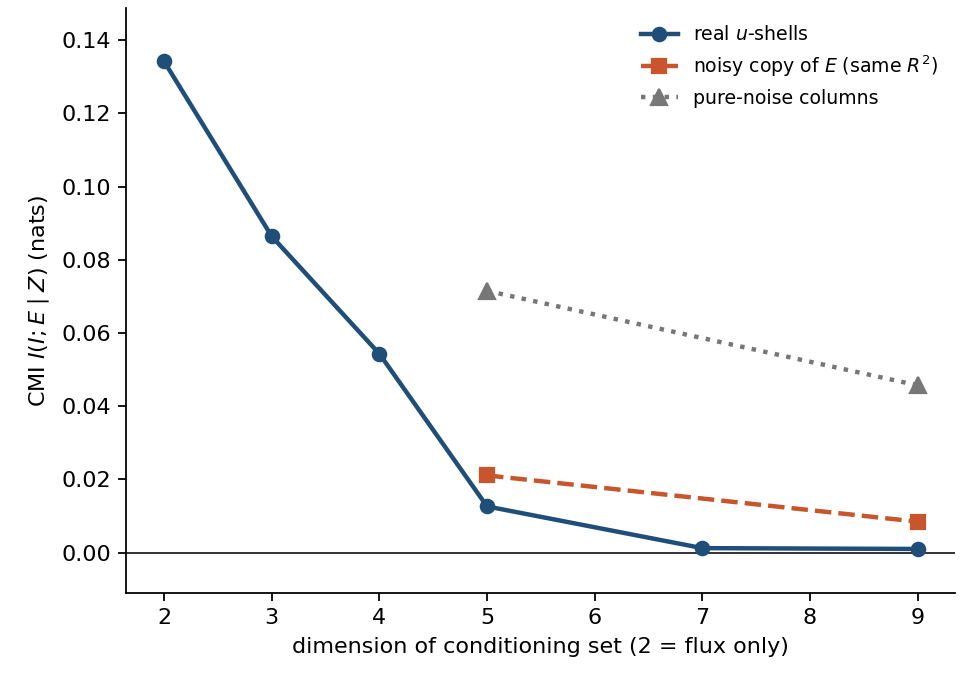
\includegraphics[width=0.7\textwidth]{u_enriched_cmi.png}
\caption{CMI $I(I;E\mid Z)$ against the dimension of the conditioning set. Real $u$-shells (blue) reduce the CMI to near zero; a noisy copy of $E$ with the same $R^2$ to $E$ (orange) does almost as well; pure-noise columns (grey) reduce it only through estimator dimension effects. The real shells therefore screen mainly because they reproduce $E$.}
\label{fig:S_u_enriched}
\end{figure}

\section{Resolution/Interior-Definition Factorial Design (Main Text \S\ref{sec:model})}
\label{sec:S_resolution_factorial}

The entries at the two resolutions use two different interior-state definitions: the $256\times256$ entries used the whole-mask adaptive-erosion definition (main text \S\ref{sec:individuation}), and the $1024\times1024$ entries used the local-distance-transform definition. Any difference between them could therefore reflect resolution, interior definition, or both.

We separate them with a full factorial design: both interior-state definitions, computed on the \emph{same} sampled simulation frames, at both resolutions, at matched production scale (single trajectory at each resolution: $\nn{\ResFramesLow}$ sampled frames at $256\times256$, $\nn{\MasterFrames}$ at $1024\times1024$), under the merge-based segmentation of \S\ref{sec:individuation} and the PC1 flux regressor of main text \S\ref{sec:ci_single_traj} (the joint two-variable regression falls outside the single-flux range in all four cells of this design; Table~\ref{tab:S_resolution_definition_2x2}).

\begin{table}[htbp]
\centering

\begin{tabular}{lcc}
\toprule
Interior definition & $256\times256$ ($N=\nn{\ResNLow}$) & $1024\times1024$ ($N=\nn{\TrajN}$) \\
\midrule
Whole-mask adaptive erosion & \rr{3}{\ResAdaptLow} & \rr{3}{\ResAdaptHigh} \\
Local-distance-transform & \rr{3}{\ResDistLow} & \rr{3}{\ResDistHigh} \\
\bottomrule
\end{tabular}
\caption{Partial correlation (PC1 flux regressor) between interior and exterior state, controlling for blanket flux, crossing spatial resolution with interior-state definition. Both definitions at a given resolution are computed on the same sampled frames, under the same merge-based segmentation (a single trajectory per resolution, hence the shared $N$ per column), so resolution and definition vary independently rather than being conflated.}
\label{tab:S_resolution_definition_2x2}
\end{table}

Holding interior definition fixed and varying resolution changes the partial correlation by \rr{1}{\ResShiftAdapt}\% (adaptive) to \rr{1}{\ResShiftDist}\% (distance-transform). Holding resolution fixed and varying interior definition changes the partial correlation by \rr{1}{\ResShiftLow}\% ($256\times256$) to \rr{1}{\ResShiftHigh}\% ($1024\times1024$). Both factors contribute modest, consistently-signed shifts of a similar order of magnitude; neither changes the sign or the order of magnitude of the result. The $256\times256$ cells use a marker spacing of 6 pixels, the equivalent of the 24 pixels used at $1024\times1024$.

\section{Supporting Checks on the Collider Diagnosis (Main Text \S\ref{sec:alt_explanations})}
\label{sec:S_mechanism_scope}

The main text's \S\ref{sec:alt_explanations} reports that the population-level conditional-independence violation does not depend on whether neighbouring organisms were fused during individuation. Among the $\rr{1}{\AltCleanPercent}\%$ of organisms for which the merge step of \S\ref{sec:individuation} fused nothing ($N=\nn{\AltCleanN}$) the flux-conditioned partial correlation is $r=\rr{3}{\AltCleanR}$, against $\rr{3}{\AltBaseline}$ for the whole single-trajectory dataset. All other numbers in this section are from that dataset at marker spacing 24 ($N=\nn{\TrajN}$). This section gives the full detail behind the follow-up checks on the conditional coupling and the collider test, summarised briefly there.

\subsection{Follow-Up Checks on the Conditional Coupling}
\label{sec:S_isolated_followups}

Three follow-up checks narrow down what this residual is not.

First, a frame-level common cause---a shared substrate field or population-wide fluctuation that varies frame to frame and drives both interior and exterior state together---would be absorbed by frame fixed effects (within-frame demeaning of $I$, $E$, and the flux regressor before computing the partial correlation, across all $\nn{\MasterFrames}$ frames). It is not: the frame-fixed-effects estimate, $r=\rr{3}{\AltFrameEffectsR}$, is essentially unchanged from the unadjusted $r=\rr{3}{\AltBaseline}$ (both computed via the single-PC1-regressor convention of \S~S2.2's footnote).

Second, adding organism radius and the seven near-field $u$-shell means (0--6, 6--12, 12--18, 18--24, 24--36, 36--48, 48--64 pixels) as covariates alongside blanket flux does not attenuate the estimate but strengthens it ($r=\rr{3}{\AltRadiusUShellsR}$). Added one at a time the $u$-shell means give partial correlations ranging from $\rr{2}{\AltUShellMax}$ to $\rr{2}{\AltUShellMin}$, with the sign changing between shells. Because the $u$-shells, the radius and the flux are strongly collinear (see \S\ref{sec:S_alt_explanations}), we regard these adjusted estimates as unstable rather than informative, and draw no conclusion from them beyond the fact that they do not remove the dependence consistently.

Third, we checked whether the single-PC1-regressor convention used throughout this section understates or inflates the violation relative to the full two-variable joint regression it was adopted in place of (see main text \S\ref{sec:ci_single_traj}): a ridge-regularised joint $(\Phi_u,\Phi_v)$ regression gives $r=\rr{4}{\AltRidgeFirst}$ to $\rr{4}{\AltRidgeLast}$ across regularisation strengths ($\alpha=0$ to $100$), stable across that range, and not overlapping the PC1-based $r=\rr{3}{\AltBaseline}$. Framed as a screened fraction of marginal shared variance against the marginal correlation ($r=\rr{4}{\AltMarginal}$), the PC1 partial corresponds to $\rr{1}{\TrajScreened}\%$ screened but the joint-regression partial to $\rr{0}{\PcTrajJointScreened}\%$: conditioning on the full two-variable flux description makes the apparent interior--exterior dependence \emph{larger}, not smaller. This is the diagnostic signature of conditioning on a collider rather than a genuine blanket state: blanket flux, by Fick's law, is computed from concentration values on both the interior and exterior side of an organism's own boundary, making it structurally a joint downstream effect of both sides rather than a state either side's dynamics act \emph{through} in Friston's sense (main text \S\ref{sec:blanket_formulation} returns to this point). The same joint estimate also falls outside the range spanned by $\Phi_u$ alone ($\rr{4}{\PcTrajFluxU}$) and $\Phi_v$ alone ($\rr{4}{\PcTrajFluxV}$)---the range check applied throughout this paper (main text \S\ref{sec:ci_single_traj})---so this is not a case the PC1 convention merely understates. We do not think this changes what the main text's \S\ref{sec:conditional_independence} two-variable flux blanket shows for the population as a whole; but flux's collider structure is a live concern that this section's checks cannot rule out, and the PC1-based $r=\rr{3}{\AltBaseline}$ should be read with that qualification.

Taken together, these checks rule out a frame-level common cause and surface a structural reason, independent of any of them, to distrust flux as the conditioning variable. For reference, the diagnostics on the full population ($N=\nn{\TrajN}$) are: marginal $r=\rr{4}{\TrajMarginal}$, flux PC1 $r=\rr{4}{\TrajPartial}$ (\rr{1}{\TrajScreened}\% screened, naive 95\% CI $[\rr{4}{\TrajNaiveLo},\rr{4}{\TrajNaiveHi}]$), flux joint $r=\rr{4}{\PcTrajJoint}$ (outside the single-flux range $[\rr{4}{\PcTrajFluxU},\rr{4}{\PcTrajFluxV}]$).

\subsection{Boundary-Concentration Collider Test and Nonlinear Confirmation}
\label{sec:S_collider_test}

The collider concern raised above makes a direct prediction: if flux's structural downstream-ness, rather than some other omitted mechanism, inflates the partial correlation, then conditioning on a variable that is a genuine state rather than a joint effect should behave differently. We tested this by recording, alongside flux, the mean $u$ and $v$ concentration over each organism's own boundary ring at that instant---a literal instantaneous state at the boundary, rather than a spatial derivative computed from both sides of it. Conditioning linearly on this pair, $(u_{\partial},v_{\partial})$, in place of flux leaves a joint partial correlation of $r=\rr{4}{\BoundJointR}$ (95\% CI $[\rr{4}{\BoundJointLo},\rr{4}{\BoundJointHi}]$), against a marginal correlation of \rr{2}{\AltMarginal}: $\rr{0}{\BoundJointRemovedPercent}\%$ of the marginal shared variance is nominally removed. This joint estimate, however, falls outside the range spanned by $u_\partial$ alone (\rr{2}{\BoundUAlone}) and $v_\partial$ alone (\rr{2}{\BoundVAlone}), and $v_\partial$ alone, the more conservative single-variable estimate, screens little. A linear partial correlation, moreover, can only detect straight-line dependence, so we repeated the test nonlinearly rather than resting on the linear result.

We estimated $\mathrm{MI}(I;E\mid \bB{})$ with the same Frenzel--Pompe/KSG estimator used throughout this paper ($k_{\mathrm{NN}}=5$, Chebyshev distance; main text \S\ref{sec:conditional_independence}), on $N=\nn{\PooledNSub}$ subsamples of the full population, for both candidate blanket variables, together with a nearest-neighbour local-shuffle null (nearest-neighbour local permutation in $\bB{}$-space)---the same null convention this paper adopts for its headline CMI check (main text \S\ref{sec:ci_cmi}). The estimator's max-norm nearest-neighbour search is scale-sensitive: a conditioning variable whose numerical range is orders of magnitude smaller than the other variables' can make no practical difference to the neighbour radius, and the estimate silently collapses towards the unconditioned value. Blanket flux, at $\sim10^{-4}$, sits three orders of magnitude below $I$, $E$, and boundary concentration ($\sim10^{-1}$ each), so we $z$-score $I$, $E$, and the conditioning variables before estimation and report the $z$-scored version throughout.

Over \nn{\PooledSubsamples} subsamples the unconditioned $\mathrm{MI}(I;E)$ is $\rr{4}{\PooledMI}\pm\rr{4}{\PooledMISE}$ nats (mean $\pm$ standard error). Properly scaled, conditioning on flux does not merely fail to screen the dependence, it \emph{increases} it: the flux-conditioned CMI is $\rr{4}{\PooledFluxCMI}\pm\rr{4}{\PooledFluxCMISE}$ nats, $\rr{0}{\PooledFluxRise}\%$ above the unconditioned value (ratio of means), and it is higher than the unconditioned value in $\nn{\PooledFluxHigher}$ of the $\nn{\PooledSubsamples}$ subsamples (individual increases from $\rr{0}{\PooledFluxRiseMin}\%$ to $\rr{0}{\PooledFluxRiseMax}\%$). In the $\nn{\PooledNullSubsamples}$ subsamples that also carry a $\nn{\PooledTrials}$-trial local-permutation null (\texttt{analyze\_pooled\_collider\_cmi.py}, seeds 0--2) the flux-conditioned CMI is $\rr{3}{\PooledFluxCMIA}$, $\rr{3}{\PooledFluxCMIB}$ and $\rr{3}{\PooledFluxCMIC}$ nats, $\rr{1}{\PooledFluxSDLo}$--$\rr{1}{\PooledFluxSDHi}$ null standard deviations above the null. Inflation, not mere non-screening, is the textbook signature expected from conditioning on a collider. Conditioning on boundary concentration instead gives $\rr{4}{\PooledBoundaryCMI}\pm\rr{4}{\PooledBoundaryCMISE}$ nats, which screens $\rr{0}{\PooledBoundaryScreened}\%$ of the dependence (ratio of means; $\rr{0}{\PooledBoundaryScreenedMean}\pm\rr{0}{\PooledBoundaryScreenedSD}\%$ per subsample), and in the null-tested subsamples it remains $\rr{1}{\PooledBoundarySDLo}$--$\rr{1}{\PooledBoundarySDHi}$ null standard deviations above its null. A candidate blanket state that removes about a fifth of the dependence and leaves the rest far outside its null is not a variable that restores conditional independence.

This qualifies the collider diagnosis rather than undermining it: flux's conditional CMI \emph{exceeding} the unconditioned value is a specific confirmation that flux behaves as a collider, and what the boundary-concentration comparison rules out is the more optimistic reading that a better-chosen blanket variable resolves the conditional-independence violation. A substantial, structured, nonlinear conditional coupling survives under the best conditioning variable we have tried. Flux remains this paper's primary operationalisation throughout, both because it has a direct physical interpretation (the literal exchange a Markov blanket is meant to mediate) and because boundary concentration's partial success should not be over-read as a privileged alternative (a caution in the same spirit as \citet{Raja2021}'s warning against fitting a candidate blanket to the very partition it is meant to test independently of).

\section{Robustness of the Statistical Approach: Full Derivation (Main Text \S\ref{sec:robustness})}
\label{sec:S_robustness}

Both the single-trajectory analyses (the main text's \S\ref{sec:conditional_independence}) and the correlation-length work (the main text's \S\ref{sec:corrlength}) treat time-separated samples from one chaotic trajectory as approximately independent draws from a common stationary distribution---an ergodicity assumption that is, in general, very difficult to establish rigorously for a nonlinear, spatially-extended system. We do not offer a formal proof; rigorous ergodicity results for stochastically-forced dissipative PDEs are a substantial mathematical research program in their own right. We instead offer computational evidence, each part designed to detect a specific, concrete failure mode.

\paragraph{Lyapunov-exponent-proxy consistency.} If the character of the chaos changed over the course of the trajectory---if the dynamics passed through qualitatively different regimes at different times---the local rate of exponential divergence between nearby trajectories should vary correspondingly. We measured this rate from three reference points widely separated in time, in one long run advanced from the settled starting field ($t=\nn{\DivRefA}$; $t=\nn{\DivRefB}$; $t=\nn{\DivRefC}$ steps after it), by branching two noise-perturbed copies from each reference state and fitting the exponential growth rate of their mean field-difference before saturation. The three estimated rates, fitted over the first $800$ steps, are \rr{4}{\DivRateOne}, \rr{4}{\DivRateTwo}, and \rr{4}{\DivRateThree} per time unit (standard deviation over mean $\nn{\DivRateSDPercent}\%$, full range $\nn{\DivRateRangePercent}\%$; Figure~\ref{fig:lyapunov}). The early part of each curve is noisy, so the rates are only moderately precise; the time for a pair to reach $90\%$ of its saturation value is a steadier comparison, and it is \nn{\DivTNinetyOne}, \nn{\DivTNinetyTwo} and \nn{\DivTNinetyThree} steps for the three references. This is consistent with, though does not prove, a single stationary chaotic regime persisting throughout. Saturation is the mean difference between two independent draws from $v$'s own spatial distribution (\rr{3}{\DivBenchOne}, \rr{3}{\DivBenchTwo}, \rr{3}{\DivBenchThree} for the three references). The burn-in used for all ensembles, $\nn{\BurninOne}$ steps, is at least twice the mean time to reach $90\%$ of it ($\nn{\DivSeparation}$ steps).

\begin{figure}[htbp]
\centering
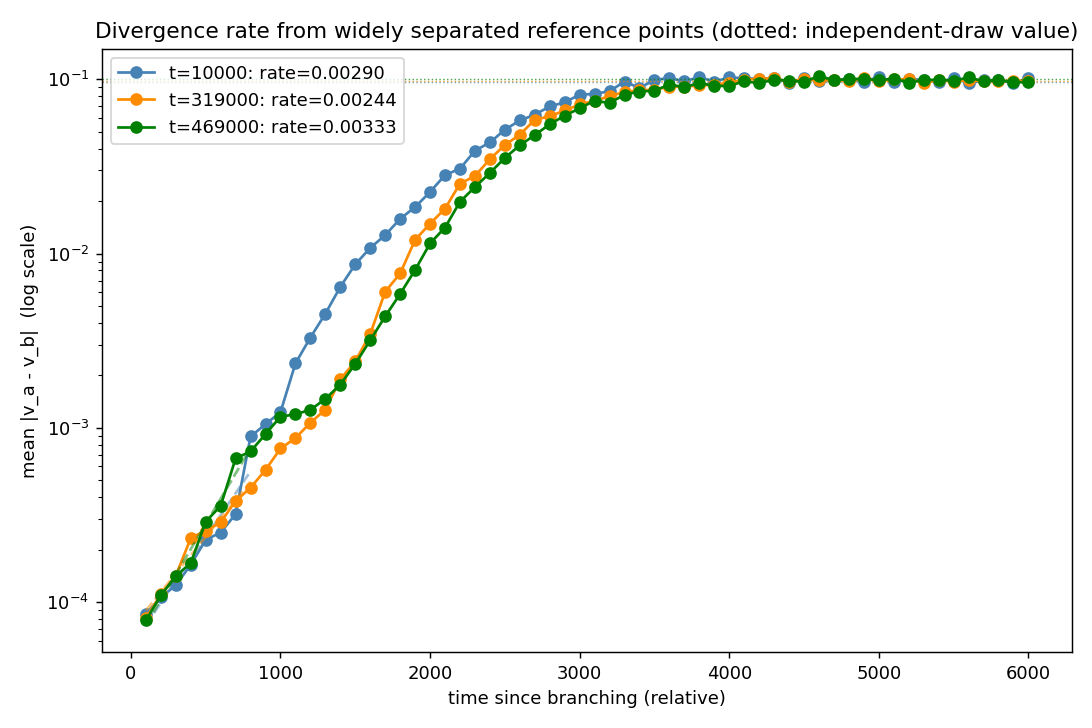
\includegraphics[width=0.75\textwidth]{lyapunov_comparison_fixed.png}
\caption{Divergence of noise-perturbed trajectory pairs branched from three reference points separated by up to \nn{\DivSpan} time units, aligned to a common relative-time origin. Offered as evidence bearing on the ergodicity assumption used throughout this paper (Section~\ref{sec:S_robustness}): if the character of the chaos changed over time, these rates and saturation times would be expected to differ substantially. Fitted exponential growth rates (first $800$ steps) are \rr{4}{\DivRateMin}--\rr{4}{\DivRateMax}, and all three pairs reach $90\%$ of the independent-draw value (dotted lines, $\approx\rr{3}{\DivBenchMin}$--$\rr{3}{\DivBenchMax}$) after \nn{\DivTNinetyMin}--\nn{\DivTNinetyMax} steps (the solver time step is $1$). The ensembles use a burn-in of $\nn{\BurninOne}$ steps, at least twice the mean separation time of $\nn{\DivSeparation}$ steps.}
\label{fig:lyapunov}
\end{figure}

\paragraph{Between-realisation correlation of population count.} The independent-ensemble check of the main text's \S\ref{sec:conditional_independence} treats its $\nn{\RunsOne}$ noise-perturbed realisations as statistically independent. Each realisation is the same settled checkpoint with its own Gaussian noise (standard deviation $10^{-3}$) added to $u$ and $v$, run for a $\nn{\BurninOne}$-step burn-in and then sampled at steps $\the\numexpr\BurninOne+100\relax$, $\the\numexpr\BurninOne+200\relax$ and $\the\numexpr\BurninOne+300\relax$. The pointwise field-divergence evidence above supports independence of the fine-grained fields, but a coarse, domain-averaged statistic such as the organism count could still decorrelate more slowly. We measured this directly with $\nn{\CountReal}$ realisations built the same way and run for $\nn{\CountSteps}$ steps, counting organisms (merged individuation, marker spacing 24) every $\nn{\CountSpacing}$ steps (\texttt{run\_count\_decorrelation.py}, \texttt{analyze\_count\_decorrelation.py}). For each non-overlapping window of eight checkpoints we computed the mean Pearson correlation between every pair of realisations' count histories, with $\pm2$ bootstrap standard errors over realisations (300 replicates). Over steps $\nn{\CountWinOneStart}$--$\nn{\CountWinOneEnd}$ the mean pairwise correlation is $\rr{3}{\CountWinOneR}\pm\rr{3}{\CountWinOneErr}$ (the noise has not yet grown). Over steps $\nn{\CountWinTwoStart}$--$\nn{\CountWinTwoEnd}$ it is $\rr{3}{\CountWinTwoR}\pm\rr{3}{\CountWinTwoErr}$. Over the later windows ($\nn{\CountWinThreeStart}$--$\nn{\CountWinThreeEnd}$, $\nn{\CountWinFourStart}$--$\nn{\CountWinFourEnd}$, $\nn{\CountWinFiveStart}$--$\nn{\CountWinFiveEnd}$, $\nn{\CountWinSixStart}$--$\nn{\CountWinSixEnd}$) it is $\rr{3}{\CountWinThreeR}$, $\rr{3}{\CountWinFourR}$, $\rr{3}{\CountWinFiveR}$ and $\rr{3}{\CountWinSixR}$, with errors of $\pm\rr{2}{\CountWinThreeErr}$ to $\pm\rr{2}{\CountWinSixErr}$. The spread of the count across realisations grows from $\rr{1}{\CountSDStart}$ organisms at the start to $\rr{1}{\CountSDLate}$ at the end. At the production burn-in of $\nn{\BurninOne}$ steps the mean pairwise correlation is $\rr{2}{\CountRAtBurnin}\pm\rr{2}{\CountRAtBurninErr}$, and it is indistinguishable from zero from about step $\nn{\CountZeroStep}$. The headline partial-correlation and CMI results are computed per organism-instance from local flux and interior/exterior state, not from population count, and the pointwise Lyapunov evidence and the close agreement between the single-trajectory and ensemble estimates (the main text's \S\ref{sec:conditional_independence}) support treating them as approximately independent at the organism-instance level. The three ensembles, which differ in sample spacing, give pooled partial correlations that differ by up to $\rr{3}{\EnsSpread}$ (\S\ref{sec:S_ensemble2}); we have not computed an effective sample size.


\paragraph{Multistability is real, and irrelevant to the patterned regime.} A purely diffuse, spatially incoherent random perturbation (small-amplitude Gaussian noise everywhere, with no localised nucleating patch) failed to produce any spots at all after 12{,}000 steps, relaxing instead to the trivial fixed point $(u,v)=(1,0)$. This confirms directly that the trivial state has a substantial basin of attraction, distinct from the patterned regime; every analysis in this paper deliberately uses a coherent nucleating seed and so never approaches this second basin. A localised patch of sufficiently large $v$ does leave the trivial state, since it nucleates spots; the trivial state's basin is large only for perturbations that contain no such patch. This is consistent with, and does not threaten, the ergodicity-within-the-patterned-regime evidence above: ergodic decomposition permits multiple disjoint components, and our claim is scoped to the one we actually sample.

Together, these results constitute empirical, though not formal, support for treating the patterned regime as a single ergodic component for the purposes of the statistics computed in this paper. A third ensemble with wider sample spacing (\S\ref{sec:S_ensemble2}) gives the same result. We have not performed formal time-window stationarity tests on the sampled distributions themselves, or tracked convergence of running statistics as a function of trajectory length (autocorrelation times of $I$, $E$ and the fluxes are in \S\ref{sec:S_autocorr}); the evidence above bears on whether the chaotic regime itself is stable, which is a necessary but not sufficient condition for the stronger ergodicity assumption these formal tests would address.

\paragraph{Clustered observations and effective sample size.} Throughout this paper, confidence intervals for partial correlations are computed treating each organism-instance as an independent observation. This is not exactly right: organism-instances sampled from the same frame share the same instantaneous field realisation and are spatially coupled to their neighbours, so naively pooling many such instances overstates the effective sample size and understates the true uncertainty.

We tested how much this matters on the single-trajectory dataset, in which every organism-instance carries the label of the frame it came from ($\nn{\MasterFrames}$ frames, $N=\nn{\TrajN}$). Pooling naively gives $r=\rr{4}{\TrajPartial}$ (95\% CI $[\rr{4}{\TrajNaiveLo},\rr{4}{\TrajNaiveHi}]$). A frame-level cluster bootstrap---resampling whole frames with replacement rather than individual organism-instances, which preserves the within-frame correlation structure a naive resample ignores---gives the interval $[\rr{4}{\ClusterBootLo},\rr{4}{\ClusterBootHi}]$ ($\nn{\ClusterN}$ clusters). The bootstrap interval is somewhat wider, confirming that clustering is real and that naive confidence intervals throughout this paper are slightly too narrow; but the qualitative conclusion is unaffected, since even the wider interval excludes zero decisively, and the naive interval lies inside it. Because consecutive frames are also serially dependent, we repeated this with a circular moving-block bootstrap, resampling runs of 5, 10, 20 and 40 consecutive frames (\texttt{run\_block\_bootstrap\_master.py}, \nn{\BlockResamples} resamples). The bootstrap standard deviation is \rr{4}{\BlockSDMin}--\rr{4}{\BlockSDMax} against \rr{4}{\BlockSDSingle} for single frames, and the widest 95\% interval ($\nn{\BlockWidestLen}$-frame blocks) is $[\rr{4}{\BlockWidestLo},\rr{4}{\BlockWidestHi}]$. Serial dependence between frames therefore adds nothing visible beyond the frame-level interval. For the ensemble, the corresponding realization-cluster bootstrap is reported in the main text's \S\ref{sec:ci_ensemble}. We did not recompute cluster-robust intervals for every statistic reported in this paper---the correlation-length curve, crowding correlations, and life-cycle averages would each need their own version of this check---and offer these targeted tests as evidence that clustering, while real, does not appear large enough to threaten the qualitative conclusions drawn throughout.

\paragraph{Nonlinear CMI under clustering.} The frame and block bootstraps above concern the linear partial correlation. The CMI null standard deviations are not cluster-adjusted, so we repeated the CMI of the main text (flux as blanket) on subsamples built to remove same-frame dependence, each compared with an ordinary random subsample of the same size (\texttt{run\_cmi\_independent\_frames.py}; three subsamples of each kind, 50 null trials each). The estimate depends on $N$, so each row is compared only with its own size. In the seed-\SeedOne\ ensemble: random $N=\nn{\IndEnsRandomN}$ gives \rr{3}{\IndEnsRandomCMI} nats (\rr{1}{\IndEnsRandomSD} null SDs); organisms at least $200$ px (about ten radii) apart within a frame, $N=\nn{\IndEnsThinnedN}$, \rr{3}{\IndEnsThinnedCMI} (\rr{1}{\IndEnsThinnedSD}); random $N=\nn{\IndEnsRandomPfN}$, \rr{3}{\IndEnsRandomPfCMI} (\rr{1}{\IndEnsRandomPfSD}); one organism per frame, $N=\nn{\IndEnsPerFrameN}$, \rr{3}{\IndEnsPerFrameCMI} (\rr{1}{\IndEnsPerFrameSD}); random $N=\nn{\IndEnsRandomPrN}$, \rr{3}{\IndEnsRandomPrCMI} (\rr{1}{\IndEnsRandomPrSD}); one organism per realisation, $N=\nn{\IndEnsPerRealN}$, \rr{3}{\IndEnsPerRealCMI} (\rr{1}{\IndEnsPerRealSD}). In the master trajectory: random $N=\nn{\IndMastRandomN}$, \rr{3}{\IndMastRandomCMI} (\rr{1}{\IndMastRandomSD}); thinned as above, $N\approx\nn{\IndMastThinnedN}$, \rr{3}{\IndMastThinnedCMI} (\rr{1}{\IndMastThinnedSD}); random $N=\nn{\IndMastRandomPfN}$, \rr{3}{\IndMastRandomPfCMI} (\rr{1}{\IndMastRandomPfSD}); one per frame, $N=\nn{\IndMastPerFrameN}$, \rr{3}{\IndMastPerFrameCMI} (\rr{1}{\IndMastPerFrameSD}). The three subsamples of one kind differ among themselves by up to about \rr{3}{\IndEnsSpreadBig} nats at the largest $N$ (ensemble) and \rr{3}{\IndMastSpreadSmall} at the smallest (master trajectory), which is larger than the difference between any scheme and its matching random subsample. Removing same-frame coupling therefore does not lower the dependence. The small-$N$ rows have little power and are consistent with, not independent confirmation of, the large-$N$ result.

\paragraph{Dataset provenance.} Sample sizes vary widely across this paper, from a few thousand to over half a million organism-instances, because different checks are built from different simulation runs, resolutions, and organism-instance definitions rather than all being subsamples of one master dataset. Table~\ref{tab:provenance} collects the main ones in one place: which simulation run each is drawn from, at what resolution and with which interior-state definition, its size, and where in the paper it is used. Because several of these datasets report a marginal or partial $I$--$E$ correlation under more than one conditioning-variable convention (the main text's \S\ref{sec:alt_explanations} in particular), Table~\ref{tab:correlation_provenance} separately collects every such correlation figure reported anywhere in this paper, alongside its source dataset and regressor convention, so that values from different datasets are not mistaken for repeated measurements of the same one.

\begin{table}[htbp]
\centering
\footnotesize

\begin{tabular}{p{3.2cm}p{0.9cm}p{1.4cm}p{1.6cm}p{4.4cm}p{1.9cm}}
\toprule
Dataset & Solver & Resolution & $N$ & Script & Used in \\
\midrule
Single trajectory ($\nn{\MasterFrames}$ frames) & PS (C) & $1024^2$ & \nn{\TrajN} & \texttt{run\_master\_trajectory.py} & \S\ref{sec:conditional_independence}, \S\ref{sec:corrlength}, \S\ref{sec:richer_blanket} \\
\quad --- CMI subsample & PS (C) & $1024^2$ & \nn{\CmiNSub} & \texttt{analyze\_master\_followups.py} & \S\ref{sec:ci_cmi} \\
\quad --- depth-sensitivity subset (\nn{\DepthFrames} frames) & PS (C) & $1024^2$ & \nn{\DepthN} & \texttt{sweep\_from\_master.py} & ESM \S\ref{sec:S_ci_support} \\
Independent ensemble, seed \SeedOne & PS (C) & $1024^2$ & \nn{\EnsOneN} & \texttt{run\_ensemble\_merged.py} & \S\ref{sec:ci_ensemble}, \S\ref{sec:friston_fe} \\
Independent ensemble, seed \SeedTwo & PS (C) & $1024^2$ & \nn{\EnsTwoN} & \texttt{run\_ensemble\_merged.py} & ESM \S\ref{sec:S_ensemble2} \\
Independent ensemble, seed \SeedThree ($\nn{\RunsThree}$ realisations; $\nn{\BurninThree}$-step burn-in, \nn{\SpacingThree}-step spacing) & PS (C) & $1024^2$ & \nn{\EnsThreeN} & \texttt{run\_ensemble\_merged.py} & ESM \S\ref{sec:S_ensemble2} \\
Timescale separation / flux asymmetry & PS (C) & $1024^2$ & \nn{\RemN} & \texttt{run\_remaining\_checks\_merged.py} & \S\ref{sec:timescale}, \S\ref{sec:flux} \\
Resolution $\times$ definition design & PS (C)/FD & $256^2$/$1024^2$ & \nn{\ResNLow} / \nn{\ResNHigh} & \texttt{run\_resolution\_2x2\_merged.py} & \S\ref{sec:model} \\
Lifecycle tracker ($\nn{\LifeSteps}$ time units) & PS (C) & $1024^2$ & \nn{\AgeN} tracked measurements; \nn{\LifeDivisions} divisions, \nn{\LifeDeaths} deaths & \texttt{run\_lifecycle.py} & \S\ref{sec:alt_explanations}, \S\ref{sec:fe_comparison} \\
Radial template $T(r)$ & PS (C) & $1024^2$ & \nn{\TrajN} profiles & \texttt{build\_template\_from\_master.py} & \S\ref{sec:template_fe} \\
Shape stability and tail decomposition ($\nn{\FramesShapeTail}$ frames) & PS (C) & $1024^2$ & \nn{\ShapeN} & \texttt{run\_shape\_stability.py}, \texttt{run\_shape\_tail\_test.py} & \S\ref{sec:timescale} \\
Level-set individuation ($\nn{\LevelFrames}$ frames of the single trajectory) & PS (C) & $1024^2$ & \nn{\LevelSingleN} / \nn{\LevelPooledN} & \texttt{level\_set\_from\_master.py}, \texttt{run\_levelset\_cmi.py} & \S\ref{sec:levelset} \\
Three-variable memory model (spacing 24) & PS (C) & $1024^2$ & \nn{\ShellNMemory} ($D_w=D_v$), \nn{\ShellNZero} ($D_w=0$) & \texttt{run\_3var\_shell\_data.py} & \S\ref{sec:threevar_blanket} \\
Divergence-rate check (three references, \nn{\DivBranch}-step branches) & PS (C) & $1024^2$ & 3 reference states, 2 perturbed copies each & \texttt{run\_\allowbreak divergence\_\allowbreak rate.py} & \S\ref{sec:S_robustness} \\
Population-count decorrelation test & PS (C) & $1024^2$ & \nn{\CountReal} realiz.\ (\nn{\CountCheckpoints} checkpoints each) & \texttt{run\_\allowbreak count\_\allowbreak decorrelation.py} & \S\ref{sec:S_robustness} \\
Substrate-enriched CMI test (master, $N=\nn{\CmiNSub}$ subsample) & PS (C) & $1024^2$ & \nn{\TrajN} & \texttt{run\_\allowbreak u\_\allowbreak enriched\_\allowbreak cmi.py} & \S\ref{sec:S_u_enriched} \\
Blanket-thickness sweep (master, $N=\nn{\CmiNSub}$ subsample) & PS (C) & $1024^2$ & \nn{\TrajN} & \texttt{run\_\allowbreak band\_\allowbreak sweep\_\allowbreak cmi.py} & \S\ref{sec:S_band} \\
Placebo-disk sweep (disks matched to the master frames, $N=\nn{\CmiNSub}$ subsample) & PS (C) & $1024^2$ & \nn{\DiskN} disks & \texttt{run\_\allowbreak random\_\allowbreak disks.py}, then \texttt{run\_\allowbreak band\_\allowbreak sweep\_\allowbreak cmi.py --data random\_\allowbreak disks.npz --tag \_disks --only-all} & \S\ref{sec:S_band} \\
Estimator cross-check against Tigramite (master, three $N=\nn{\CmiNSub}$ subsamples) & PS (C) & $1024^2$ & \nn{\TrajN} & \texttt{run\_\allowbreak cmi\_\allowbreak crosscheck.py} & ESM \S\ref{sec:S_cmi_calibration} \\
CMI on subsamples without same-frame coupling (ensemble seed \SeedOne and master) & PS (C) & $1024^2$ & \nn{\EnsOneN} / \nn{\TrajN} & \texttt{run\_\allowbreak cmi\_\allowbreak independent\_\allowbreak frames.py} & ESM \S\ref{sec:S_robustness} \\
Null calibration (random-forest conditional surrogate of master, \nn{\CalReplicates} replicates, $N=\nn{\CalSub}$) & PS (C) & $1024^2$ & \nn{\TrajN} & \texttt{run\_\allowbreak null\_\allowbreak calibration.py} & ESM \S\ref{sec:S_cmi_calibration} \\
\bottomrule
\end{tabular}
\caption{Provenance of the main datasets used throughout this paper. ``Distance transform'' is the local-distance-transform interior definition of the main text's \S\ref{sec:individuation}; all datasets use the merge-corrected watershed with marker spacing 24 pixels unless noted. ``PS (C)'' is the pseudo-spectral solver with the C/FFTW backend; ``FD'' is the original finite-difference solver. Scripts are described in Table~\ref{tab:S_repro_table}.}
\label{tab:provenance}
\end{table}

\begin{table}[htbp]
\centering
\footnotesize

\begin{tabular}{p{4.6cm}p{1.5cm}p{1.0cm}ccc p{1.7cm}}
\toprule
Dataset & $N$ & Regr.\ & Marginal $r$ & Partial $r$ & Screened & Used in \\
\midrule
Single trajectory, $1024^2$ & \nn{\TrajN} & PC1 & \rr{3}{\TrajMarginal} & \rr{3}{\TrajPartial} & $\rr{1}{\TrajScreened}\%$ & \S\ref{sec:conditional_independence} \\
\quad unmerged organisms & \nn{\AltCleanN} & PC1 & \rr{3}{\AltCleanMarginal} & \rr{3}{\AltCleanR} & $\rr{1}{\AltCleanScreened}\%$ & \S\ref{sec:alt_explanations} \\
\quad flux, joint two-variable & \nn{\TrajN} & Joint & \rr{3}{\TrajMarginal} & \rr{3}{\PcTrajJoint} & $\rr{0}{\PcTrajJointScreened}\%$ & \S\ref{sec:S_isolated_followups} \\
\quad frame fixed effects & \nn{\TrajN} & PC1 & \rr{3}{\TrajMarginal} & \rr{3}{\AltFrameEffectsR} & $\rr{0}{\AltFrameScreened}\%$ & \S\ref{sec:S_alt_explanations} \\
\quad + local crowding density & \nn{\TrajN} & PC1 & \rr{3}{\TrajMarginal} & \rr{3}{\AltCrowding} & $\rr{0}{\AltCrowdScreened}\%$ & \S\ref{sec:S_alt_explanations} \\
\quad + radius only (no flux) & \nn{\TrajN} & --- & \rr{3}{\SizeMarginalTwo} & \rr{3}{\SizeRadiusOnlyTwo} & --- & \S\ref{sec:S_alt_explanations} \\
\quad + radius \& eccentricity, with flux & \nn{\TrajN} & PC1 & \rr{3}{\TrajMarginal} & \rr{3}{\AltRadiusEccentricity} & ill-posed & \S\ref{sec:S_alt_explanations} \\
Independent ensemble, seed \SeedOne & \nn{\EnsOneN} & PC1 & \rr{3}{\EnsOneMarginal} & \rr{3}{\EnsOnePartial} & $\rr{1}{\EnsOneScreened}\%$ & \S\ref{sec:ci_ensemble} \\
Independent ensemble, seed \SeedTwo & \nn{\EnsTwoN} & PC1 & \rr{3}{\EnsTwoMarginal} & \rr{3}{\EnsTwoPartial} & $\rr{1}{\EnsTwoScreened}\%$ & ESM \S\ref{sec:S_ensemble2} \\
Independent ensemble, seed \SeedThree & \nn{\EnsThreeN} & PC1 & \rr{3}{\EnsThreeMarginal} & \rr{3}{\EnsThreePartial} & $\rr{1}{\EnsThreeScreened}\%$ & ESM \S\ref{sec:S_ensemble2} \\
Age-confound, lineage-tracked & \nn{\AgeN} & PC1 & --- & \rr{3}{\AgeBaseline} & --- & \S\ref{sec:alt_explanations} \\
\quad with age as covariate & \nn{\AgeN} & PC1 & --- & \rr{3}{\AgeWithAge} & --- & \S\ref{sec:S_alt_explanations} \\
\quad age terciles (young / mid / old) & \nn{\AgeYoungN} / \nn{\AgeMidN} / \nn{\AgeOldN} & PC1 & --- & \rr{3}{\AgeYoungR} / \rr{3}{\AgeMidR} / \rr{3}{\AgeOldR} & --- & \S\ref{sec:S_alt_explanations} \\
\quad lineage fixed effects & \nn{\AgeN} & PC1 & --- & \rr{3}{\LineageWithinR} & --- & \S\ref{sec:S_alt_explanations} \\
Resolution factorial, $1024^2$ (adaptive / distance transform) & \nn{\ResNHigh} & PC1 & --- & \rr{3}{\ResAdaptHigh} / \rr{3}{\ResDistHigh} & --- & \S\ref{sec:model} \\
Resolution factorial, $256^2$ (adaptive / distance transform) & \nn{\ResNLow} & PC1 & --- & \rr{3}{\ResAdaptLow} / \rr{3}{\ResDistLow} & --- & \S\ref{sec:model} \\
Level-set individuation, single-maximum & \nn{\LevelSingleN} & PC1 & \rr{3}{\LevelSingleMarginal} & \rr{3}{\LevelSingleR} & $\rr{0}{\LevelSingleScreened}\%$ & \S\ref{sec:levelset} \\
\quad pooled w/ recovered pairs & \nn{\LevelPooledN} & PC1 & \rr{3}{\LevelPooledMarginal} & \rr{3}{\LevelPooledR} & $\rr{0}{\LevelPooledScreened}\%$ & \S\ref{sec:levelset} \\
\bottomrule
\end{tabular}
\caption{Every marginal and partial $I$--$E$ correlation figure reported in this paper, by dataset, so that figures computed on different datasets are not mistaken for repeated measurements of the same quantity. ``Regressor'' is the blanket-conditioning convention: ``Joint'' is the two-variable $(\Phi_u,\Phi_v)$ regression; ``PC1'' is the single leading-principal-component regressor used as the reference convention, because the joint value lies outside the range of the single-flux values (main text \S\ref{sec:ci_single_traj}). A ``---'' under Marginal $r$ means the marginal correlation was not separately reported for that dataset. ``Screened'' is $1-(r_{\text{partial}}/r_{\text{marginal}})^2$; a negative value means conditioning \emph{increased} the apparent dependence. All screened figures here are \emph{linear} only; the nonlinear conditional-mutual-information checks (ESM \S\ref{sec:S_collider_test}) find that flux conditioning \emph{increases} the nonlinear dependence in every population tested, so the linear screened fractions should not be read as evidence that flux screens the dependence.}
\label{tab:correlation_provenance}
\end{table}


\section{Supporting Checks for the Free-Energy Comparison (Main Text \S\ref{sec:fe_comparison})}
\label{sec:S_fe_comparison}

The lifecycle tracker underlying every check in this section follows merge-fused organisms (main text \S\ref{sec:individuation}), the same individuation as the cross-sectional analyses; a division is a fused organism that becomes two non-overlapping organisms persisting through the $\nn{\LifeConfirmWindow}$-time-unit confirmation window (\S\ref{sec:falsestarts}). Every $N$ reported in this section refers to this convention. The Friston $\mathcal{F}$ in every check below uses the generative model refit on the seed-\SeedOne\ ensemble ($N=\nn{\EnsOneN}$; \texttt{fe\_model.py}), and the template $T(r)$ is built from the merge-fused organisms of the single-trajectory run (\S\ref{sec:S_template_procedure}).

\subsection{Held-Out Template Check for Circularity}
\label{sec:S_fe_heldout}

As a further check on whether the close agreement between $\mathcal{F}_{\text{template}}$ and the Friston $\mathcal{F}$ (the main text's \S\ref{sec:fe_comparison}) is circular---both quantities are, after all, ultimately built from statistics of the same underlying population---we repeated the comparison using a $T(r)$ template built from a separate simulation, the single-trajectory run ($\nn{\TrajN}$ merge-fused organisms), which is disjoint from both the ensemble used to fit the Friston $\mathcal{F}$ generative model and the lifecycle-tracker simulation used for the main comparison. Using only the pre-division portion of each of the $\nn{\HeldDivisions}$ confirmed divisions (the full pre-and-post-division curve used in the main comparison requires additional reconstruction we did not repeat here) and a simpler relative-time binning, the correlation between the two quantities remains strong, $r=\rr{3}{\HeldMin}$--$\rr{3}{\HeldMax}$ depending on bin width ($r=\rr{3}{\HeldROne}$, $\rr{3}{\HeldRTwo}$, $\rr{3}{\HeldRThree}$, $\rr{3}{\HeldRFour}$ with $\nn{\HeldBinsOne}$, $\nn{\HeldBinsTwo}$, $\nn{\HeldBinsThree}$ and $\nn{\HeldBinsFour}$ matched bins at $\nn{\HeldWidthOne}$, $\nn{\HeldWidthTwo}$, $\nn{\HeldWidthThree}$ and $\nn{\HeldWidthFour}$ time-unit widths respectively). This is below the main comparison's $r=\rr{3}{\FeMatchedR}$; the two analyses differ in more than the template (pre-division only, coarser bins), so we do not read the difference as a failure to replicate. The check confirms that the convergence is not an artefact of fitting and evaluating both quantities on the same data: it survives when the template is built entirely independently of the comparison it is evaluated against.

\subsection{Instance-Level Agreement and Confound Check}
\label{sec:S_fe_instance}

A further concern is that the main comparison is conducted entirely at the level of population-averaged curves---about $\nn{\FeMatchedBins}$ relative-time bins---rather than individual organism-instances, and that any two quantities trending together over a life cycle will correlate strongly once smoothed this way, regardless of how tightly they track each other measurement by measurement. We tested this directly at the instance level: for every individual organism-instance in the lifecycle tracker with a valid $(I,E,\Phi_u,\Phi_v)$ measurement---not only those in the aligned, binned division window plotted in the main text's Figure~\ref{fig:fe_comparison}, but every tracked instance across both confirmed divisions and still-active lineages ($N=\nn{\InstN}$)---we computed $\mathcal{F}_{\text{template}}$ and the Friston $\mathcal{F}$ directly, using the same template and the same fitted generative-model parameters as the main comparison, and correlated the two without any relative-time binning or averaging. The instance-level correlation is $r=\rr{3}{\InstR}$ (bootstrap 95\% CI $[\rr{3}{\InstLo},\rr{3}{\InstHi}]$)---weaker than the $r=\rr{3}{\FeMatchedR}$ obtained after binning and averaging, which is what one would expect if binning removes real measurement-to-measurement noise rather than manufacturing a spurious relationship, but still a strong, decisively nonzero instance-level agreement in its own right. We then asked whether both quantities simply track organism size. A radial-distance proxy for size (the distance to each organism's own profile minimum) correlates only $\rr{2}{\FeSizeProxyR}$ with the measured equivalent radius $\sqrt{\text{area}/\pi}$, so we control for the measured area of every instance (\texttt{run\_fe\_size\_control.py}; median equivalent radius $\rr{1}{\FeSizeMedian}$ px, interquartile range $\rr{1}{\FeSizeQLo}$--$\rr{1}{\FeSizeQHi}$ px). Both free energies correlate with equivalent radius ($\mathcal{F}_{\text{template}}$ \rr{2}{\FeSizeRTemplate}, Friston $\mathcal{F}$ \rr{2}{\FeSizeRFriston}), as do the fluxes ($\Phi_u$ \rr{2}{\FeSizeRFluxU}, $\Phi_v$ \rr{2}{\FeSizeRFluxV}); $I$ and $E$ much less (\rr{2}{\FeSizeRI}, \rr{2}{\FeSizeRE}). The dependence on size is nonlinear, so the form of the control matters:
\begin{center}\small
\begin{tabular}{lc}
\hline
Control & $r(\mathcal{F}_{\text{template}},\mathcal{F})$\\
\hline
None & \rr{3}{\FeSizeRZero}\\
Age & \rr{3}{\FeSizeAge}\\
Radial-distance proxy & \rr{3}{\FeSizeProxy}\\
Equivalent radius, linear & \rr{3}{\FeSizeRLinear}\\
Equivalent radius, cubic & \rr{3}{\FeSizeRCubic}\\
Cubic radius and age & \rr{3}{\FeSizeCubicAge}\\
Cubic radius, log area and age & \rr{3}{\FeSizeCubicLogAge}\\
\hline
\end{tabular}
\end{center}
Within quintiles of equivalent radius the correlation is \rr{2}{\FeSizeStratumOne}, \rr{2}{\FeSizeStratumTwo}, \rr{2}{\FeSizeStratumThree}, \rr{2}{\FeSizeStratumFour} and \rr{2}{\FeSizeStratumFive} from the smallest to the largest stratum (about $\nn{\FeSizeStratumN}$ instances each; mean \rr{2}{\FeSizeStrataMean}). Splitting the Friston $\mathcal{F}$ into its state (KL) term and its flux (accuracy) term, both correlate with $\mathcal{F}_{\text{template}}$ (\rr{2}{\FeSizeKLF} and \rr{2}{\FeSizeAccF}) and both track size (\rr{2}{\FeSizeKLReq} and \rr{2}{\FeSizeAccReq}). So the instance-level agreement is partly a shared dependence on size, and a large part of it remains after the control. We report no confidence interval for these partial correlations: instances within a lineage are not independent. What remains is agreement between two functions of the same measured state, and it does not show that either is inference. A split-half check of the generative-model fit, comparing $\mathcal{F}$ computed from the full-dataset fit with $\mathcal{F}$ computed from a model fit on the other half of the data, gives $r=\rr{6}{\FeHeldOutR}$ (to six decimals), so the Friston $\mathcal{F}$ values do not depend on the particular data used to fit the model.


\section{Supporting Discussion: Scope and Critical-Literature Engagement (Main Text \S\ref{sec:blanket_formulation}--\ref{sec:critical_lit})}
\label{sec:S_discussion_scope}

\subsection{Coarse Graining and the Data Processing Inequality (Main Text \S\ref{sec:blanket})}
\label{sec:S_coarse}

Throughout, $I$ and $E$ are low-dimensional summaries of the full interior and exterior field configurations, not those configurations themselves: the nearest-neighbour conditional-mutual-information estimator used below (the main text's \S\ref{sec:conditional_independence}) could not be run on the full fields directly even in principle, since nonparametric mutual-information estimation degrades sharply with dimension and the full fields have far more degrees of freedom than any feasible dataset could constrain. This coarsening is licensed by a two-sided form of the data processing inequality: for variables $X,Y$ and any functions $F,G$ applied separately to each---each free to use its own private randomness, but not to see the other variable---$\mathrm{MI}(X;Y)\ge \mathrm{MI}(F(X);G(Y))$, and the same holds conditionally, $\mathrm{MI}(X;Y\mid Z)\ge \mathrm{MI}(F(X);G(Y)\mid Z)$, for $Z$ held fixed on both sides \citep{CoverThomas2006}. Taking $X,Y$ to be the full interior and exterior states and $F,G$ the maps that reduce them to $I,E$, this makes any measured $\mathrm{MI}(I;E\mid \bB{})$ a rigorous lower bound on the corresponding quantity for a richer description of interior and exterior, for the same blanket $\bB{}$: a positive finding cannot be an artefact of discarding information on the $I$/$E$ side, since discarding information can only shrink this quantity, never inflate it. This guarantee assumes $F$ and $G$ act on $X$ and $Y$ separately. The watershed masks that define $I$ and $E$ depend on the whole field, including neighbouring organisms, so the bound strictly holds for a mask assignment that does not depend on $I$ or $E$'s own values, a reasonable but unverified premise. It gives no protection to $\bB{}$ itself, since conditioning is not processing in the inequality's sense: blanket flux behaves as a statistical collider that \emph{increases} apparent dependence (the main text's \S\ref{sec:blanket_formulation}). The choice of blanket variable is therefore tested empirically (the main text's \S\ref{sec:ci_cmi} and \S\ref{sec:richer_blanket}).

\subsection{What Formulation of the Markov Blanket Does This Test? Full Discussion (Main Text \S\ref{sec:blanket_formulation})}
\label{sec:S_blanket_formulation}

The Markov blanket literature is not univocal about which formal object the conditional-independence condition is a claim about, and our own operationalisation (the main text's \S\ref{sec:conditional_independence}) makes several choices that are worth stating explicitly rather than leaving implicit. \citet{Bruineberg2022} make a version of this point at the level of the whole framework, distinguishing a purely statistical, Pearl-style Markov blanket \citep{Pearl1988}---a conditional-independence structure read directly off a joint distribution, with no further requirement---from Friston's dynamical blanket, which additionally constrains how influence flows between the partitioned states over time and is meant to license the inferential interpretation. Our central test (the main text's \S\ref{sec:conditional_independence}) targets the statistical structure directly---exactly the Pearl-style question of whether $I\perp E\mid \bB{}$ holds for the joint density---and a fortiori bears on the stronger dynamical claim only to the extent that the latter requires the former as a precondition, which it does; a system failing to have even a statistical blanket cannot have a dynamical one either, though the converse does not hold. The five points below sharpen this general observation into specific, concrete choices our own operationalisation makes.

\paragraph{A summary of a summary.} As the caption of Figure~\ref{fig:schematic} notes, $I$ and $E$ are themselves coarse-grained summaries of the full internal and external states ($I \subsetneq \mu_{\text{full}}$, $E \subsetneq \eta_{\text{full}}$), and the blanket state $\bB{}=(\Phi_u,\Phi_v)$ is a comparably drastic reduction of whatever the full boundary field carries. These two coarsenings are not symmetric in what they cost the paper's argument. Because the central finding is a \emph{violation}---$\mathrm{MI}(I;E\mid \bB{})$ decisively greater than zero---the data processing inequality (the main text's \S\ref{sec:blanket}) guarantees that a richer description of $I$ and $E$ could only show an equal or larger violation, never a smaller one: the coarse-graining on that side is conservative rather than a liability, and there is no need to repeat the test on higher-dimensional interior/exterior descriptions to know what they would show. No such guarantee covers $\bB{}$: conditioning is not processing in the inequality's sense, and a poorly-chosen or overly coarse blanket variable can inflate apparent dependence as readily as it can hide real screening, exactly as the main text's \S\ref{sec:blanket_formulation}'s collider discussion documents. The enrichment tests of the main text's \S\ref{sec:richer_blanket} address the coarsening of $\bB{}$ directly. Adding the organism's own $v$-shells does not shrink the violation (the linear version is ill-conditioned). Adding substrate $u$-shells that lie inside the exterior ring removes it, but only because those shells reproduce $E$ (ESM \S\ref{sec:S_u_enriched}). A band of the surrounding field about one organism radius thick, with $E$ placed beyond it, screens the interior to under $0.01$ nats and at most $3.7$ null standard deviations (ESM \S\ref{sec:S_band}). The violation is therefore a property of thin, boundary-defined blankets in this system, not of every conceivable blanket variable.

\paragraph{Flux as a possible collider.} A further choice worth stating explicitly is what kind of object blanket flux is. Friston's formal blanket is meant to be a state that internal and external processes act \emph{through}---a genuine causal intermediary. Boundary flux, computed via Fick's law ($J=-D\nabla C$) from the field values immediately inside and outside an organism's own boundary, is instead a joint downstream function of both sides at that instant: structurally closer to a collider than to a mediating state. Conditioning on a collider can induce or inflate statistical dependence between its causes rather than screen it, and this is not merely hypothetical here. Properly scaled, the nonlinear conditional mutual information given flux exceeds the unconditioned value: \rr{3}{\ScaleTrajZ} against \rr{3}{\ScaleTrajRaw} nats in the single-trajectory subsample (\rr{0}{\ScaleTrajGainPercent}\%; ESM \S\ref{sec:S_collider_test}). Synergy can also raise a conditional mutual information, so this is consistent with collider structure rather than proof of it. Mass balance gives a second reason for caution: the inward $u$-flux tracks the integrated reaction rate over the organism's mask (ESM \S\ref{sec:S_uv2_flux}), so flux partly reads out the interior's own size and activity. Conditioning on boundary concentration, a genuine state, helps only a little: it screens about \rr{0}{\PooledBoundaryScreened}\% of the nonlinear dependence. We have not found a boundary-defined variable free of this problem; the band of the main text's \S\ref{sec:richer_blanket} shows what screening by a thicker layer of the field looks like.

\paragraph{Equal-time versus path-wise screening.} The test in the main text's \S\ref{sec:conditional_independence} is an equal-time one: at each sampled instant, we ask whether the joint distribution of $(I,E)$ factorises conditional on $\bB{}$ measured at that same instant. This is a claim about the stationary density, not about dynamics. A separate, stronger reading is path-wise: for a local PDE, the interior's future can depend on the exterior's history only through the boundary field's own history, so a defender could ask instead whether the interior's trajectory is independent of the exterior's trajectory given the boundary's trajectory, a property of the process rather than of a single-time slice. Both readings appear in the FEP literature, usually without being distinguished explicitly. We test only the equal-time version; the path-wise version would require conditioning on an entire history of $\bB{}$ rather than its instantaneous value, a qualitatively different and more demanding empirical test that we have not attempted. It is worth noting that a static, instantaneous flux measurement is a weak proxy for path-wise screening in particular: a boundary process with its own memory could satisfy equal-time independence while still carrying dependence through its history, or vice versa, so the two readings are not simply nested in difficulty. The three-variable memory model of the \S\ref{sec:threevar} gives the boundary chemistry itself a short relaxation time, but $\tau_w=\eps^2$ is, as noted there, far too fast to constitute a meaningful test of path-wise screening at the relevant timescale; it bears on whether an internal memory affects the equal-time result---which it does not appreciably in the far field, though \S\ref{sec:threevar_blanket} finds it changes the near-boundary value only modestly (\rr{2}{\ShellInnerMemory} against \rr{2}{\ShellInnerPlain} in the innermost shell)---not on whether path-wise screening holds.

\paragraph{Deterministic dynamics.} Friston's construction (the main text's \S\ref{sec:fep_intro}) assumes a random dynamical system possessing a nonequilibrium steady-state density, with the blanket condition stated as a property of that density. Our simulations are deterministic PDEs; noise enters, at most, once at initialisation (the main text's \S\ref{sec:conditional_independence}), with every subsequent step governed by the main text's Eqs.~2--3 exactly. The single-trajectory test (the main text's \S\ref{sec:conditional_independence}) accordingly probes the empirical distribution of a deterministic, chaotic trajectory over time, not a stochastic process's steady-state density in the sense the theorem is stated for; the independent-ensemble test addresses only the dependence of our result on single-trajectory ergodicity (the main text's \S\ref{sec:robustness}), not this distinct scope question. A defender of the framework could reasonably argue that a purely deterministic system, however chaotic, falls outside the class of systems the theorem was proven for, and that our result says nothing about the stochastic case it actually concerns. We think this gap is narrow in practice---a chaotic attractor's natural invariant measure plays much the same role here that a stochastic steady-state density plays in the theorem, and the qualitative picture we find (a dependence concentrated within about one organism radius of the boundary) is not obviously a fact about determinism specifically---but we have not closed it directly. A fluctuating-hydrodynamics variant of the Gray--Scott system, with continuous thermal-strength noise rather than a single initial perturbation \citep{Kim2017,Kim2018}, would test the stochastic case the theorem is actually stated for, and is a natural, tractable extension we have not undertaken here.

\paragraph{A state-dependent partition.} Watershed segmentation recomputes each organism's boundary, at every frame, from the current field configuration, including its neighbours' current states (the main text's \S\ref{sec:individuation}). Friston's partitions, by contrast, are formally fixed index sets, chosen once and applied uniformly; \citet{Friston2013} himself flags the resulting ambiguity, in his discussion of blankets that must be identified on ``wandering sets'' rather than fixed coordinates, as an unresolved technical difficulty for exactly this kind of self-organising, boundary-redefining system. Conditioning on a quantity whose own definition depends on the current joint state of the system can, in principle, induce statistical dependence through the conditioning procedure itself, independently of any physical channel connecting interior and exterior. This cannot be the whole explanation: the violation persists among the \rr{1}{\AltCleanPercent}\% of organisms that individuate on their own, where no merge step has fused neighbours (the main text's \S\ref{sec:alt_explanations}), and under a level-set construction that shares no construction with watershed (the main text's \S\ref{sec:levelset}). But the level-set boundary is state-dependent in the same sense (its threshold crossing depends on the current field), so it does not resolve this point. The failure we report is therefore a failure of this particular, state-dependent, and arguably most natural partition, which is a related but logically separate claim from the failure of fixed-partition blankets in general.

\subsection{Further Critical Literature Omitted from the Main Text}
\label{sec:S_more_lit}

The free energy principle has been extended from single organisms to nested hierarchies of blankets spanning molecules to societies \citep{Kirchhoff2018}, and applied to biological pattern formation and morphogenesis, illustrated with simulations of planarian regeneration and axial polarity, by \citet{Kuchling2020}, whose construction assumes rather than tests the relevant conditional-independence structure and which drew critical commentary \citep{Annila2020,Bizzarri2020}. \citet{HeinsDaCosta2022} discuss technical aspects of the \citet{Aguilera2022} result, and \citet{Biehl2021} raise concerns about how timescale-separation arguments are typically used to justify blanket partitions. \citet{VirgoEgbertFroese2011}, working within autopoietic theory, argue that a system's spatial boundary should not be conflated with its operational limits, the network of constitutive processes that make it up, which need not be confined within that boundary (their examples are conceptual, such as a thermostat whose feedback loop runs through the room it regulates). Their claim concerns which processes count as part of an organism, not whether a boundary's value depends on a neighbour, but it belongs to the same critique of treating an organism's boundary as intrinsic. \citet{Krakauer2020} offer a complementary information-theoretic framework for what makes something an individual, of which the watershed-segmented organisms here can be read as one concrete instance. \citet{Friston2021Stochastic} use a Helmholtz decomposition and polynomial expansion to construct a Laplace (Gaussian) approximation to the steady-state density of two coupled Lorenz systems (six ODEs, non-spatial), identifying a blanket from the zero entries of the resulting Hessian, an existence result for that approximated low-dimensional system. \citet{Friston2013} suggests, as a natural extension of his simulations, blankets that dissipate and reform cyclically; self-replicating reaction-diffusion spots are a fully specified system in which a version of that question can be posed.

For Gray--Scott spots with small diffusivity ratio $\delta$ ($D_u=1$, $D_v=\delta^2$), matched-asymptotic theory predicts spots that drift slowly relative to the chemistry \citep{Reynolds1994,Reynolds1997,Kolokolnikov2009}. Our parameters have $\delta^2=D_v/D_u=\rr{1}{\DvOverDu}$, far outside that regime, yet the timescale separation of the main text's \S\ref{sec:timescale} persists. We do not claim numerical equivalence between $\rho$ and the theory's timescales.

\subsection{Relation to the Critical Literature: Full Discussion (Main Text \S\ref{sec:critical_lit})}
\label{sec:S_critical_lit}

\citet{Raja2021} argue that the Markov blanket formalism can be imposed on essentially any system after the fact---the ``Markov blanket trick''---rendering the framework's claims difficult to falsify. Our results sharpen rather than settle this concern. In the weakest, near-tautological sense in which Friston sometimes uses the term publicly (any bounded, persisting structure that exchanges material with an environment, as opposed to a sealed equilibrium abstraction), our organisms trivially qualify, and nothing here challenges that reading. But the strict, mathematical sense that actually does explanatory work---conditional independence of internal and external states given the blanket, the antecedent that would need to hold before the inference interpretation could even be considered---is testable, and we have tested it directly, in a concrete nonlinear system, and found it false for the boundary-defined variables we tested. This is, we believe, a concrete instance of exactly the kind of empirical test the Markov-blanket-trick critique argues is rarely performed: not an a priori argument about whether the formalism \emph{could} apply, but a direct measurement of whether the required statistical structure is \emph{actually present}. \citeauthor{Raja2021} raise a further, more conceptual concern along the way: that Markov blanket partitions are insensitive to \emph{relational features} (properties that are inherently about an organism's relationship to its surroundings, not a pure internal state) and to \emph{constitutive self-organisation} (how a living system actively builds and maintains its own boundary, rather than having a boundary given to it in advance). Our individuation is itself relational, since watershed boundaries are drawn relative to neighbours, and the merge correction (\S\ref{sec:S_individuation}) shows how a partition choice becomes entangled with the state of the neighbours. We do not claim a mechanism for the conditional coupling beyond what the main text shows: it is concentrated within about one organism radius of the boundary (the main text's \S\ref{sec:richer_blanket}) and persists among organisms that individuate on their own (the main text's \S\ref{sec:alt_explanations}). Whether a relational or constitutive feature in the sense \citeauthor{Raja2021} intend explains it remains an open candidate that these checks neither support nor displace.

This same non-uniqueness is acknowledged by Friston himself. \citet{Friston2013} explicitly notes that a system generally admits a multitude of nested Markov blanket partitions---an animal's blanket encloses those of its organs, cells, and nuclei---and that, formally, every such partition licenses the same inferential interpretation, asking directly whether this implies lifelike behaviour is ubiquitous, or whether something specific distinguishes the blankets of systems considered alive. His own speculative answer proposes a criterion: that the special, biological blankets are those of minimum entropy, whose constituent states change slowly relative to what they separate---precisely the timescale-separation property we test directly in the main text's \S\ref{sec:timescale}. Our organisms satisfy this proposed criterion robustly by the direct positional measure $\rho$ (median \rr{3}{\RemRhoMedian}), though, as noted in the main text's \S\ref{sec:timescale}, a stricter relative-autocorrelation-time comparison leaves its strict form only partly resolved; and they exhibit lifelike behaviour by any ordinary use of the term---growth, self-replication, competition, death---yet the conditional-independence property this criterion is meant to identify still fails for the boundary-defined variables we tested. This is a sharper result than a general observation that partitions are non-unique: it is a direct test of Friston's own proposed resolution to that non-uniqueness, on a system satisfying the resolution's stated condition, that comes out negative.

A further point is worth making explicit. That some untested, sufficiently elaborate partition of the state space might restore conditional independence is true of any system, in any finite empirical test, and proves too little on its own: taken as a general objection to claims of blanket-absence, it would apply equally to blanket-presence claims made without testing every alternative partition, and would make the entire question empirically unaddressable in either direction. The relevant question is not whether such a partition exists in the abstract, but whether one exists that could be motivated on grounds other than rescuing the hypothesis. The candidates we test here are not arbitrary in this sense: flux across a physically-motivated boundary, a substantially enriched local near-field description, and boundaries constructed by an entirely different, non-watershed method are the kinds of partition a researcher would actually propose, and---as shown above---satisfy Friston's own proposed criterion for a biologically special blanket. Failure of these thin, boundary-defined candidates is a meaningful result even though it cannot, and does not purport to, exhaust the space of conceivable ones. A field band about one organism radius thick does screen (\S\ref{sec:S_band}), so the question is not whether some partition screens but what may be concluded from it.

This raises a further question distinct from artefact-versus-genuine: even granting that the violation is real, is it large enough to matter, or is the blanket approximately screening in a sense the strict test cannot credit? As reported in the main text's \S\ref{sec:conditional_independence}, conditioning on blanket flux (PC1) removes about $\rr{0}{\ScreenedMin}$--$\rr{0}{\ScreenedMax}\%$ of the marginal linear shared variance ($r^2$ from \rr{3}{\TrajRsqMarginal} to \rr{3}{\TrajRsqPartial} in the single trajectory, \rr{3}{\EnsOneRsqMarginal} to \rr{3}{\EnsOneRsqPartial} in the ensemble), and under the nonlinear estimator it removes none, raising the conditional mutual information from \rr{3}{\PooledMI} to \rr{3}{\PooledFluxCMI} nats. A defender of the framework could reasonably describe the linear figure as an approximately-screening blanket, in the spirit of the literature on weak or approximate Markov blankets (e.g.\ \citealt{Sakthivadivel2022}), rather than a system with no blanket at all. We do not think this reading rescues the strict inferential interpretation, for three reasons that are independent of the coupling's size. First, the coupling is not noise: it has real, reproducible spatial structure (the main text's \S\ref{sec:corrlength}), concentrated within about one organism radius of the boundary, and only a band of that thickness removes it (the main text's \S\ref{sec:richer_blanket}); it is not reduced by boundary-defined variables, including the boundary's own concentration. Second, the coupling persists, changing in magnitude and not in kind, across the individuation methods, resolutions and estimators we tried (the claims map at the start of this supplement), which is not what a single-method artefact would look like. Third, and most importantly, exact conditional independence is not required for the variational free energy of the main text's \S\ref{sec:friston_fe} to remain a valid upper bound on surprisal: that bound holds for any approximate posterior $q$ and any generative model $p$, blanket or no blanket, as our own construction in the main text's \S\ref{sec:friston_fe} illustrates directly. What exact screening buys, in Friston's construction, is a different and stronger claim: the step from a system's internal states to \emph{beliefs about external states}, in which the internal states are licensed to be read as parameterising an approximate posterior over the actual external states, via the conditional synchronisation map that Friston's derivation of the free energy principle relies on. Without conditional independence, the mathematical bound survives, but the quantity it bounds no longer has this inferential reading attached to it: the internal states can still be fit to look like they are minimising a free energy functional (the main text's \S\ref{sec:fe_comparison} shows they can, closely), without that fit meaning the organism is thereby performing approximate Bayesian inference about anything outside its boundary. Whether ``approximately screening, with a real, structured conditional coupling that only a thick band of the field removes'' is close enough to license the belief-encoding reading is, in the end, a question about how much slack that stronger claim can absorb before its interpretation changes in kind; we think the honest answer is that it cannot absorb this much for the thin, boundary-defined variables, but we report the magnitudes explicitly so readers can weigh that question themselves.

Boundary concentration screens about $\rr{0}{\PooledBoundaryScreened}\%$ of the nonlinear dependence and flux inflates it (\S\ref{sec:S_collider_test}). Whatever degree of approximate screening a reader is inclined to credit to this system, no thin, boundary-defined variable we tested provides it.

Our results also connect to \citet{Aguilera2022}'s findings, in weakly-coupled linear stochastic systems: that the Markov blanket condition requires special, non-generic sparse coupling and holds only approximately for weak coupling, and, more consequentially, that even when a valid blanket and decoupled solenoidal flow are present, the averaged flow the FEP's own mathematics requires does not track a system's actual dynamics---their own numerical example shows the two diverging outright. Our system is fully nonlinear and far from the weak-coupling regime their theorem addresses, so we do not claim a direct extension of it; but the qualitative conclusion---that a sparse, thin partition satisfying the strict conditional-independence criterion may be uncommon, and that even a nominal blanket does not straightforwardly license the inferential interpretation the framework wants to draw from it---is consistent with our thin-blanket result, though a thick band of the field does screen (\S\ref{sec:S_band}) and so the genericity question is left open, and lends further support to the caution we raise in the main text's \S\ref{sec:freeenergy} against reading a well-behaved Friston free energy as evidence of genuine inference.

\citet{Friston2021Stochastic} attack a closely related question from the opposite methodological direction: rather than testing a candidate partition empirically, they parameterise the nonequilibrium steady-state density of a low-dimensional chaotic system (two coupled Lorenz systems, six ODEs) analytically, using a Helmholtz decomposition and polynomial expansion, to identify a Markov blanket from the resulting Laplace (Gaussian) approximation. That approach is, in principle, more powerful where it applies---it characterises the full density rather than testing one candidate partition against data---but it has so far been demonstrated only for a low-dimensional, non-spatial system, and the blanket it identifies is a property of the Gaussian approximation rather than a claim about the original nonlinear dynamics. Our spatially-extended, many-body system has no comparably tractable density; a direct empirical test of a candidate partition, as we perform here, is the practical alternative in that regime. The two approaches are complementary rather than competing, and both point the same direction: establishing that a Markov blanket actually exists, even in a fully specified, comparatively simple nonlinear system, requires real technical work and cannot be assumed.

It is worth being precise about where Friston himself has located the disagreement with this critical literature, since it bears directly on what kind of system ours is. In a direct reply to \citet{Raja2021}, \citeauthor{FristonUltimateTrick2022} \citep{FristonUltimateTrick2022} concedes the core point explicitly: ``the core claim of Raja et al.\ is that the FEP is a principle or method, which (heuristically) allows us to say that, if a system has a Markov blanket, then we can model its dynamics as a path of least surprisal or, equivalently, as minimising a free energy functional of Bayesian beliefs. This seems uncontroversial to me.'' \citep[p.~10]{FristonUltimateTrick2022} His defence against \citet{Aguilera2022} and \citet{Biehl2021} is not that their mathematics is wrong, but that they ``deal with the wrong kind of systems (usually, linear edge cases),'' and that genuine Markov blankets should be expected generically as system size and nonlinearity grow, citing \citet{Sakthivadivel2022}'s argument that the probability of a sufficiently large, sparsely-coupled system \emph{lacking} a blanket tends to zero. Our system is precisely the kind this defence points to: not a linear edge case, not small, and not analytically simplified---a fully nonlinear, many-body, spatially-extended population of thousands of interacting units. If the genericity argument is right, this is close to an ideal candidate for a blanket to emerge in practice. We find that thin, boundary-defined variables do not provide one, while a band of the field about one radius thick does, as local coupling would produce. The thin-blanket failure therefore does not refute the genericity reply. What remains in dispute is the synchronisation condition and the inferential reading, which our blanket test does not address.

The question of whether an internal memory is compatible with a Markov blanket has itself been addressed theoretically by \citet{ParrMemory2021}, who pose essentially the question we test empirically in the \S\ref{sec:threevar}: if all dependence between a system and its surroundings must pass through the blanket, how can a system retain a memory of its past without violating the independence condition? Their resolution treats memory-induced coupling as \emph{transient}---a perturbation to blanket states induces a temporary conditional dependency that relaxes back towards the steady-state independence condition, rather than a permanent departure from it. Our finding that adding an explicit chemical memory channel has little effect on the long-run, many-frames-averaged correlation structure (the \S\ref{sec:threevar}) is consistent with, though does not directly confirm, this picture: a purely transient effect would be expected to leave exactly this kind of steady-state average largely unchanged, which is what we observe.

\section{A Three-Variable Model with Chemical Memory (Main Text \S\ref{sec:richer_blanket})}
\label{sec:threevar}

Does giving an organism a real internal memory---a private, slowly-relaxing internal state, of the kind one might naively expect to support a more clearly individuated identity---bring the system closer to satisfying the Markov blanket condition? We constructed a minimal, chemically well-motivated extension to test this.

\subsection{Derivation}

We replace the irreversible trimolecular step $U + 2V \to 3V$ with two bimolecular steps \citep{BarasPearsonMansour1990,BarasMansourPearson1996,Lefever1988,Kim2017,Kim2018}: a catalytic step $U + W \to V + W$ and a reversible dimerisation $2V \rightleftharpoons W$, with rate constants parametrised by a single small parameter $\eps$:
\begin{align}
\frac{\partial u}{\partial t} &= -\frac{1}{\eps} uw + F(1-u) + D_u \nabla^2 u, \\
\frac{\partial v}{\partial t} &= \frac{1}{\eps} uw - \frac{2}{\eps} v^2 + \frac{2}{\eps^2} w - (F+k)v + D_v \nabla^2 v, \\
\frac{\partial w}{\partial t} &= \frac{1}{\eps} v^2 - \frac{1}{\eps^2} w + D_w \nabla^2 w,
\end{align}
with $D_w = D_v = 10^{-5}$ throughout (the dimer $W$ taken to diffuse at the same rate as its monomer $V$, in the absence of a more specific physical rationale). Setting $\partial w/\partial t = 0$ gives the quasi-steady state $w_{\text{qss}} = \eps v^2$, and substituting back, the catalytic term becomes $\frac{1}{\eps} u (\eps v^2) = uv^2$ \emph{exactly}, with no separate amplitude-matching required: as $\eps \to 0$, this system recovers standard Gray--Scott (Eqs.~\ref{eq:gs_u}--\ref{eq:gs_v}) exactly. Linearising $\partial w/\partial t$ near quasi-equilibrium shows the relaxation time of this memory variable is $\tau_w = \eps^2$, independent of the amplitude scaling; at $\eps=0.25$, for instance, $\tau_w = 0.0625$, more than two orders of magnitude faster than the $v$-relaxation timescale $\tau \approx \rr{1}{\Tau}$ of main text \S\ref{sec:timescale}, consistent with $w$ tracking its quasi-steady state closely even at this comparatively large $\eps$. As $\eps \to 0$, $w$ becomes simultaneously vanishingly small in amplitude and infinitely fast to relax; finite $\eps$ introduces a real, first-principles chemical memory of finite duration.

\subsection{Numerical Schemes}
\label{sec:threevar_numerics}

The reverse rate $1/\eps^2$ is stiff for small $\eps$. Because this term is purely local (no spatial coupling), it can be treated implicitly at negligible cost, without a sparse matrix solve: writing the $w$-update with the linear reverse term evaluated at the new time step gives
\begin{equation}
w_{n+1} = \frac{\eps^2 w_n + \Delta t\, \eps\, v_n^2 + \Delta t\, \eps^2 D_w \nabla^2 w_n}{\eps^2 + \Delta t},
\end{equation}
with $u$ and $v$ updated explicitly thereafter, using $w_{n+1}$ for the stiff (reverse-reaction) contribution to $\partial v/\partial t$ and $w_n$ for the (non-stiff) catalytic contribution. This renders only the stiff local reverse term unconditionally stable; the diffusion terms (for $u$, $v$, and $w$ alike, the last evaluated explicitly at $w_n$ above) and the remaining reaction terms are still handled explicitly and retain their own standard stability constraints. In practice this finite-difference scheme was stable at $\Delta t = 1$ for every $\eps$ tested at $256\times256$, indicating those remaining explicit constraints were not binding at this resolution, though we did not separately verify timestep convergence at each $\eps$. This is the scheme used for the order-disorder scan described below.

For the $D_w=0$ vs.\ $D_w=D_v$ comparison of \S\ref{sec:threevar_blanket}, run at $1024\times1024$ for direct comparability with the rest of this paper's primary results, we instead extend the pseudo-spectral scheme described in the ESM, \S\ref{sec:S_pseudospectral}: the same stiff local reverse-term update above is retained unchanged (it involves no spatial coupling and so is resolution-independent), but diffusion for all three fields is handled via the exact ETD integrating factor rather than an explicit Laplacian, applied as a separate step immediately after the reaction update (a first-order Lie splitting, matching the accuracy level already used elsewhere in this paper). We validated this against the finite-difference scheme the same way as described there: branching both from an identical $256\times256$ state and comparing after 20 steps, where the two agreed closely (the comparison was a one-off check made while building the solver, and the finite-difference code for the three-variable model is not part of the archived code; the quantitative differences are therefore not reported here). The spectral scheme is needed to reach $1024\times1024$, where an explicit treatment of $w$'s diffusion would not be stable at $\Delta t=1$.

Scanning $\eps \in \{0.1, 0.25, 0.5, 1.0\}$ at the same $(F,k)$ used throughout, with $D_w=D_v$, we find a sharp order-disorder transition: sustained chaos at $\eps=0.1$ and $\eps=0.25$ gives way to a slowly-relaxing, near-perfect hexagonal lattice by $\eps=0.5$, and a static, sparse (23-organism), non-replicating lattice by $\eps=1.0$. This is not driven by the memory timescale approaching $v$'s own---even at $\eps=1$, $\tau_w/\tau_v\approx0.073$, more than an order of magnitude too fast for that---but by an amplitude effect, which can be made explicit: writing $w = w_{\text{qss}} + \delta w$ and eliminating the fast variable $w$ adiabatically (\S\ref{sec:threevar}'s $\tau_w=\eps^2$ justifies treating $\delta w$ perturbatively in $\eps$), the leading correction is $\delta w \approx \eps^3\left(D_w\nabla^2 v^2 - 2v\,\partial v/\partial t\right)$, which enters the $v$-equation multiplied by its $2/\eps^2$ coefficient there, giving an $O(\eps)$ correction to the $v$-kinetics of the form
\begin{equation}
(1+4\eps v)\,\frac{\partial v}{\partial t} \approx uv^2 - (F+k)v + D_v\nabla^2 v + 2\eps D_w \nabla^2 v^2 + O(\eps^2),
\label{eq:threevar_correction}
\end{equation}
i.e.\ an effective rescaling of the local $v$-relaxation rate by a factor of $(1+4\eps v)^{-1}\approx1-4\eps v$, plus a diffusive-transport correction proportional to $\eps D_w$. Both terms grow with $\eps$, and by $\eps\sim0.5$ this evidently suffices to move the effective kinetics out of the parameter region supporting chaotic replication at this particular $(F,k)$. A regime combining long chemical memory with sustained chaos may require a different point in $(F,k)$ space than the one investigated here; we do not attempt that broader search in this paper.

\subsection{Effect on the Blanket Violation}
\label{sec:threevar_blanket}

Repeating the correlation-length measurement of main text \S\ref{sec:corrlength}---$r(s)$, here for the $\eps=0.25$ three-variable model---at $1024\times1024$ with the pseudo-spectral solver, current individuation (marker spacing 24, merged organisms), the same shell schedule, and the plain Gray--Scott baseline of main text \S\ref{sec:corrlength} ($N=\nn{\TrajN}$), we find two different outcomes depending on whether $W$ diffuses (Figure~\ref{fig:memory_comparison}).

\textbf{$D_w=D_v$} ($N=\nn{\ShellNMemory}$ organism-instances; organism-size coefficient of variation \rr{3}{\ShellCVMemory}). The violation stays in a boundary layer. The partial correlation is $r=\rr{2}{\ShellInnerMemory}$ in the innermost shell (\rr{1}{\ShellInnerRadii} organism radii), against $\rr{2}{\ShellInnerPlain}$ for plain Gray--Scott, so memory does not make the near-boundary violation deeper here. It is then \rr{2}{\ShellMemNearOne} at \rr{1}{\ShellMemNearOneAt} radii and \rr{2}{\ShellMemNearThree} at \rr{1}{\ShellMemNearThreeAt} radii, and is between \rr{3}{\ShellMemFarLo} and \rr{3}{\ShellMemFarHi} from 7 radii out to 15. Plain Gray--Scott is \rr{2}{\ShellPlainNearHi} to \rr{2}{\ShellPlainNearLo} between 1 and 3 radii and between \rr{2}{\ShellPlainFarLo} and \rr{2}{\ShellPlainFarHi} beyond 7 radii. Giving $W$ the same diffusion as $V$ therefore changes the sign of the correlation at 1--3 radii but neither removes the violation at the boundary nor extends it.

\textbf{$D_w=0$.} The pattern does not remain a replicating population. In a run from the settled two-variable state ($\nn{\ShellNZero}$ organism-instances, to $t=108{,}000$) the organism count was 283 at every frame printed, the mean organism radius was \rr{1}{\ShellRadiusZero} px, and the coefficient of variation of organism size was \rr{3}{\ShellCVZero} (against \rr{3}{\ShellCVMemory} for $D_w=D_v$). That is a near-regular lattice of almost identical organisms, with essentially no births or deaths, similar to the ordered lattices found at larger $\eps$ above. In this state the correlation $r(s)$ oscillates between about \rr{2}{\ShellZeroMin} and \rr{2}{\ShellZeroMax} with the lattice spacing (right panel of Figure~\ref{fig:memory_comparison}); that follows from every organism having neighbours at the same distances, and we do not read it as a measure of memory.

We conclude that chemical memory, in the form tested, does not remove the blanket violation at the organism boundary, and that when $W$ cannot diffuse the system freezes into a lattice at this $(F,k)$ and $\eps$, so that no statement about long-range coupling can be made for it. We did not search other parameter values for a regime that combines non-diffusing memory with sustained replication.

\begin{figure}[htbp]
\centering
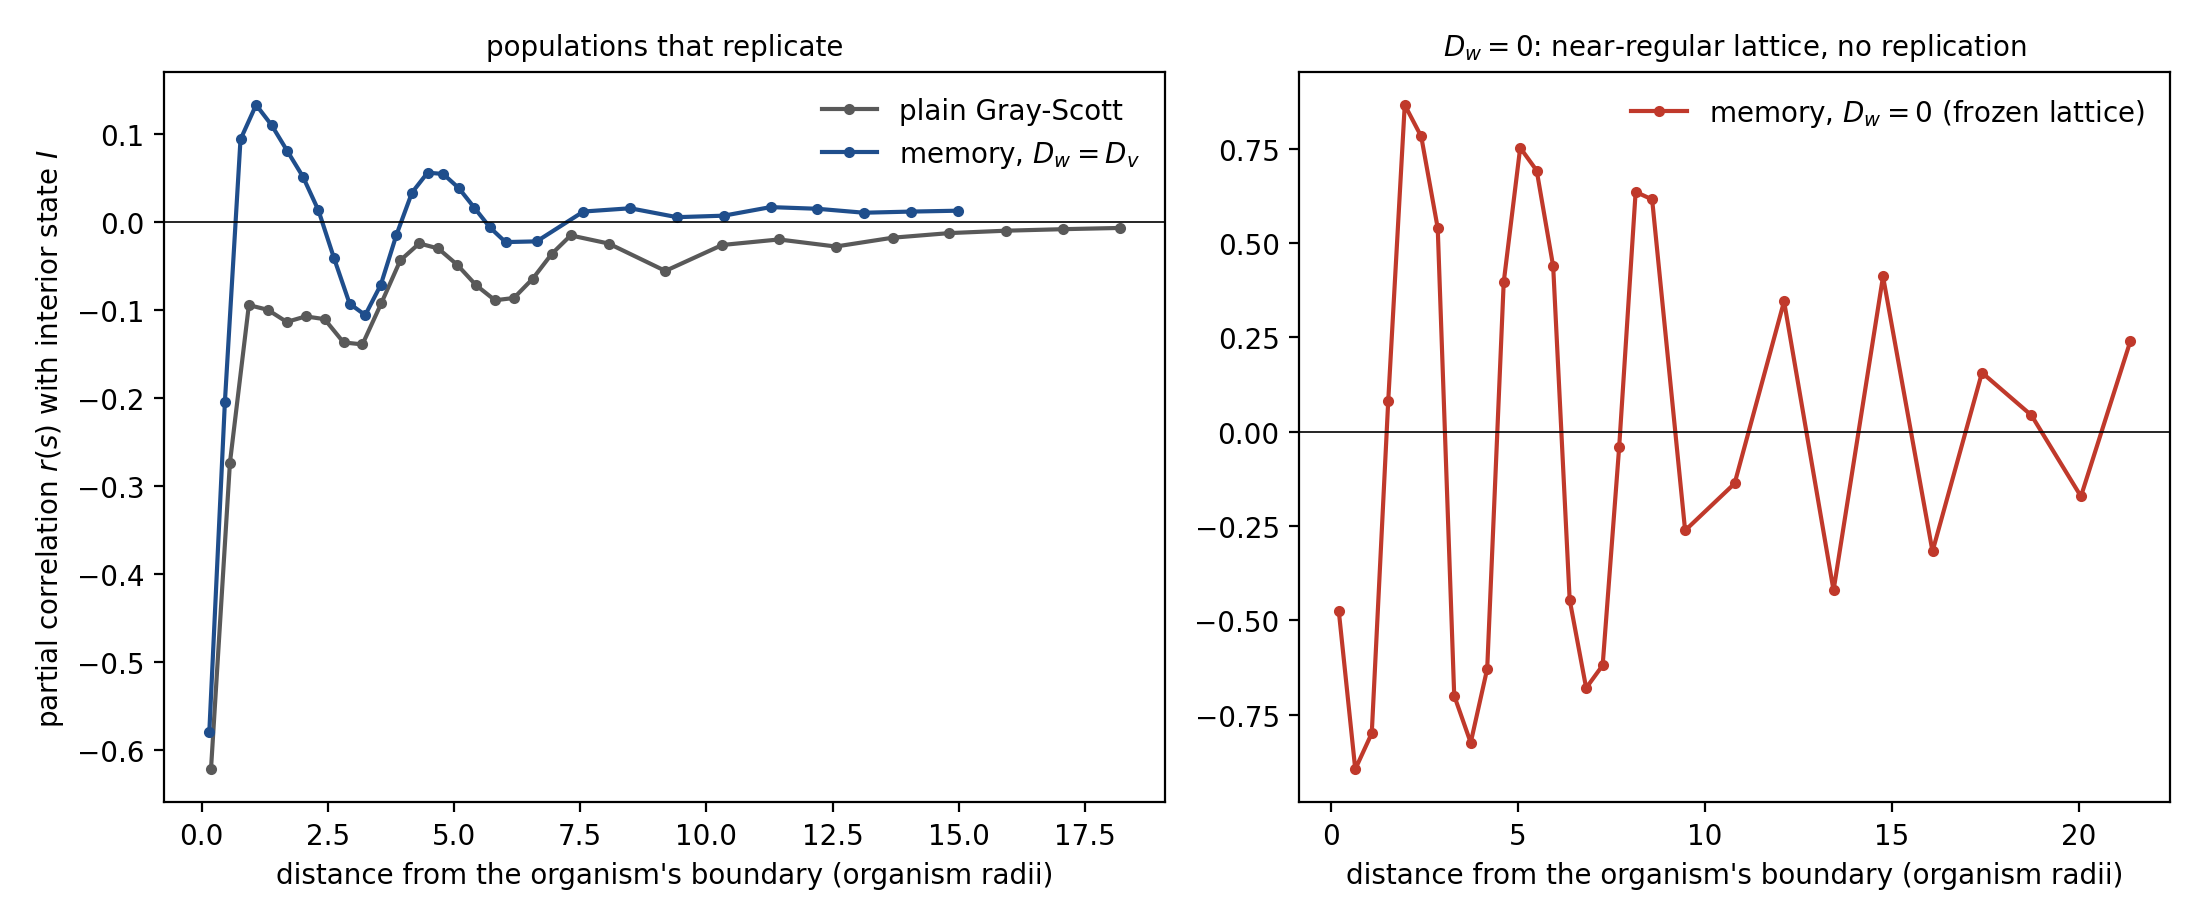
\includegraphics[width=\textwidth]{memory_comparison_1024.png}
\caption{Correlation length at $\eps=0.25$, all at $1024\times1024$ with marker spacing 24. Left: plain Gray--Scott ($N=\nn{\TrajN}$) and the memory model with $D_w=D_v$ ($N=\nn{\ShellNMemory}$), both populations that replicate. Right: the memory model with $D_w=0$ ($N=\nn{\ShellNZero}$), which freezes into a near-regular lattice of 283 organisms; its oscillations follow the lattice spacing.}
\label{fig:memory_comparison}
\end{figure}

\section{Total Reaction Rate and Boundary Flux (Main Text \S\ref{sec:fe_comparison})}
\label{sec:S_uv2_flux}

Conservation of $u$ over an organism's mask gives, in the quasi-steady limit, outward $u$-flux $=-\Delta x^2\big[\sum uv^2 - F\sum(1-u)\big]-\Delta x^2\,\tfrac{d}{dt}\sum u$, where $\Delta x$ is the grid spacing. The inward flux should therefore track the total reaction rate $\sum uv^2$, less the feed supplied inside the mask. We tested this on the lifecycle record at $1024\times1024$ ($\nn{\MassN}$ organism-instances, all lifecycles; \texttt{check\_\allowbreak flux\_\allowbreak massbalance.py}, reading \texttt{lifecycle\_progress.pkl}). The $u$-flux is inward for every instance. The inward flux correlates $r=\rr{3}{\MassR}$ with the total $uv^2$ and $r=\rr{3}{\MassRArea}$ with area; the total $uv^2$ correlates $r=\rr{3}{\MassRUvArea}$ with area. After removing area from both, the partial correlation is \rr{3}{\MassPartial}, and inside deciles of area the correlation is \rr{3}{\MassDecileLo}--\rr{3}{\MassDecileHi}. A fit of inward flux on total $uv^2$ alone has $R^2=\rr{3}{\MassFitRsq}$ with a coefficient \rr{2}{\MassCoefOne} of $\Delta x^2=\num{\MassDx}$ ($L=\rr{1}{\Lval}$, $n=\nn{\gridn}$). The balance explains this: the feed term $F\sum(1-u)$ ($F=\rr{3}{\MassFeed}$ for this run) is about half the reaction term, because the mean $u$ inside an organism is about $0.4$. The prediction with no fitted numbers, $\Delta x^2[\sum uv^2-F\sum(1-u)]$, gives a median measured-to-predicted ratio of \rr{3}{\MassRatio} over all instances. Its correlation with the measured flux ($r=\rr{3}{\MassRPred}$) is lower than that of the total $uv^2$ alone (\rr{3}{\MassR}), because the two large terms nearly cancel and the unrecorded term $\tfrac{d}{dt}\sum u$ then matters more. A two-coefficient fit on $\sum uv^2$ and $\sum(1-u)$ is unstable: the two sums are nearly collinear (both scale with organism size), and it returns $c_1/\Delta x^2=\rr{2}{\MassCoefTwo}$. We therefore rely on the no-fit prediction. On a single settled frame ($185$ organisms, \texttt{checkpoint\_\allowbreak 1024\_\allowbreak settled.npz}) the identity holds to machine precision and $\sum du/dt$ is small (median $-0.5$ against $27$ for $\sum uv^2$), so the system is close to steady state.

\section{Surprisal of the Boundary Flux and the Gap to the Friston $\mathcal{F}$ (Main Text \S\ref{sec:fe_comparison})}
\label{sec:S_surprisal}

With the linear-Gaussian generative model of main-text \S\ref{sec:friston_fe}, $o=(\Phi_u,\Phi_v)\sim\mathcal{N}(A\mu_p+b,\ \Sigma+\sigma_p^2AA^{\top})$, so the surprisal $-\ln p(o)=\ln 2\pi+\tfrac12\ln|\Sigma+\sigma_p^2AA^{\top}|+\tfrac12(o-m_o)^{\top}(\Sigma+\sigma_p^2AA^{\top})^{-1}(o-m_o)$ is exact. The posterior given the flux is Gaussian with precision $1/\sigma_p^2+A^{\top}\Sigma^{-1}A$, and the gap is $\mathrm{KL}(q\|p(s\mid o))$ between two one-dimensional Gaussians. The identity $\mathcal{F}=-\ln p(o)+\text{gap}$ holds to $\num{\SurprIdentity}$ over the $\nn{\SurprN}$ organism-instances with finite $I$, $E$, $\Phi_u$, $\Phi_v$ in the confirmed divisions (and to $10^{-9}$ on random Gaussian models, as a test of the code). Both covariance matrices are well conditioned (condition numbers \rr{0}{\SurprCondSigma} and \rr{0}{\SurprCondTotal}), so the near-collinearity of $\Phi_u$ and $\Phi_v$ does not cause numerical trouble here. The fitted constants are $\mu_p=\rr{4}{\SurprMuP}$, $\sigma_p^2=\num{\SurprSigmaP}$, $A=(\num{\SurprAOne},\num{\SurprATwo})\times10^{-4}$, $b=(\num{\SurprBOne},\num{\SurprBTwo})\times10^{-5}$, slope \rr{3}{\SurprSlope} and intercept \rr{3}{\SurprIntercept} for $\mu_q(I)$, and $\sigma_q^2=\num{\SurprSigmaQ}$ (refit live by \texttt{fe\_model.py}). Mean $\mathcal{F}=\rr{2}{\SurprMeanF}$, mean surprisal \rr{2}{\SurprMeanS}, mean gap \rr{3}{\SurprMeanGap} nats (median \rr{3}{\SurprGapMedian}, 95th percentile \rr{3}{\SurprGapPctNinetyFive}, maximum \rr{2}{\SurprGapMax}); the absolute values depend on the arbitrary flux units. At instance level the correlation of $\mathcal{F}$ with surprisal is \rr{3}{\SurprRInstance}, with area \rr{2}{\SurprRAreaF} (surprisal \rr{2}{\SurprRAreaS}, gap \rr{2}{\SurprRAreaG}). Division-aligned and averaged over the $N=\nn{\HeldDivisions}$ confirmed divisions ($\nn{\SurprBins}$ matched bins, Figure~\ref{fig:surprisal}), surprisal correlates with $\mathcal{F}$ at \rr{3}{\SurprRCurve}, with $\mathcal{F}_{\mathrm{template}}$ at \rr{3}{\SurprRTemplate} and with area at \rr{3}{\SurprRAreaCurve}; the gap correlates with $\mathcal{F}$ at \rr{3}{\SurprRGapF}. The gap peaks about $\nn{\SurprGapPeakTime}$ time units before division (about \rr{2}{\SurprGapPreDivision} nats) and is lowest just after it (about \rr{3}{\SurprGapPostMin}).

\begin{figure}[htbp]
\centering
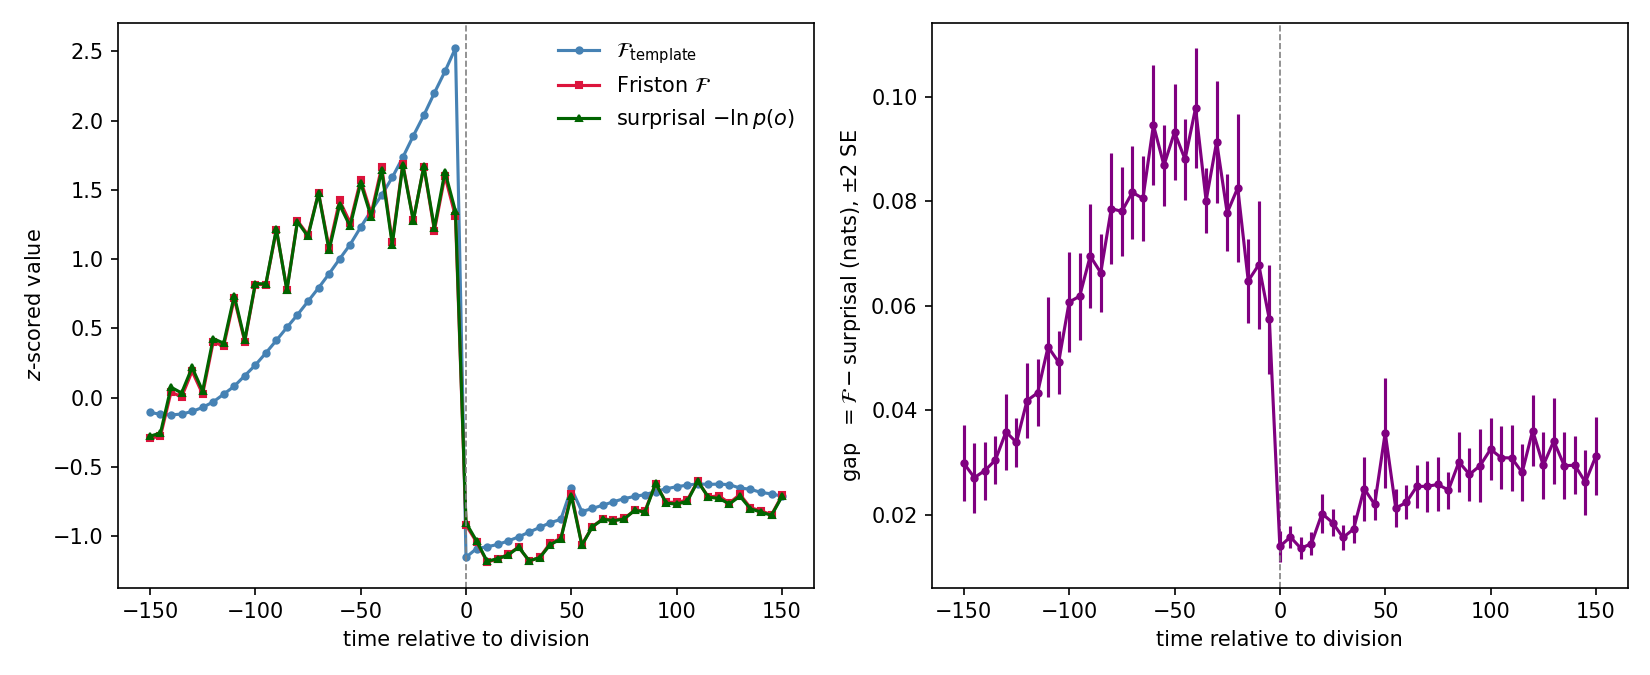
\includegraphics[width=\textwidth]{fe_surprisal_1024.png}
\caption{Left: $z$-scored division-aligned curves of $\mathcal{F}_{\mathrm{template}}$, the Friston $\mathcal{F}$ and the surprisal $-\ln p(o)$; the last two coincide. Right: the gap $\mathcal{F}-(-\ln p(o))$ in nats, mean $\pm2$ standard errors.}
\label{fig:surprisal}
\end{figure}

\section{Lineage Tracking, False-Start Rejection, and Lifespan Distribution (Main Text \S\ref{sec:fe_comparison})}
\label{sec:S_lineage}

\subsection{Distinguishing Real Divisions from Transient Deformations}
\label{sec:falsestarts}

Because watershed segmentation is a purely geometric criterion, it cannot distinguish a spot that is genuinely dividing from one that transiently deforms into a peanut shape and relaxes back without dividing. Naively counting every detected one-becomes-two event as a division contaminates population statistics, including specifically the correlation-length results (a peanut-shaped, not-yet-separated pair is exactly the geometry the merge-based individuation of main text \S\ref{sec:individuation} is designed to fuse into one organism-instance).

We resolve this with an explicit lineage tracker with delayed confirmation. Before settling on a final procedure, we first ran an exploratory pass with no confirmation logic at all, simply recording how long a detected split persisted before either the two children re-merged or one died independently, in order to determine a sensible confirmation window empirically (Figure~\ref{fig:duration_hist}): remerge durations cluster below 30 time units, while durations ending in a child's later, independent death cluster in the hundreds, well separated from the remerge population. Based on this, our final procedure holds every detected one-becomes-two event (via frame-to-frame overlap matching, requiring both putative children to claim $>25\%$ of the parent's area) \emph{pending}: neither the parent's death nor the children's births are written to any permanent record. The episode resolves as:
\begin{itemize}
\item \textbf{False start}, immediately, if the two children re-merge into a single watershed region. Nothing is recorded; the original parent lineage continues uninterrupted under its original identity.
\item \textbf{Confirmed division}, immediately, if one child dies with no forward match at all before the confirmation window elapses (this already proves the two children were genuinely distinct individuals).
\item \textbf{Confirmed division}, once a fixed confirmation window (50 time units, chosen from the empirical bimodal-ish separation between remerge durations, which cluster below 30 time units, and division-to-independent-death durations, which cluster in the hundreds; Figure~\ref{fig:duration_hist}) elapses with neither outcome.
\end{itemize}
Only upon confirmation are the parent's death and both children's births (at age zero, at the moment of the original split) written to the permanent lifespan record.

At $1024\times1024$ the procedure is applied to merge-fused organisms (\S\ref{sec:individuation}): a division is a fused organism that becomes two non-overlapping organisms that persist through the confirmation window. Over \nn{\LifeSteps} time units it records \nn{\LifeDivisions} confirmed divisions and \nn{\LifeDeaths} deaths (\nn{\LifeCompleted} completed lifecycles). We do not report a false-start rate at $1024\times1024$. The 50-time-unit confirmation window was chosen from the division-duration distribution of Figure~\ref{fig:duration_hist}, measured on a $256\times256$ run.

\begin{figure}[htbp]
\centering
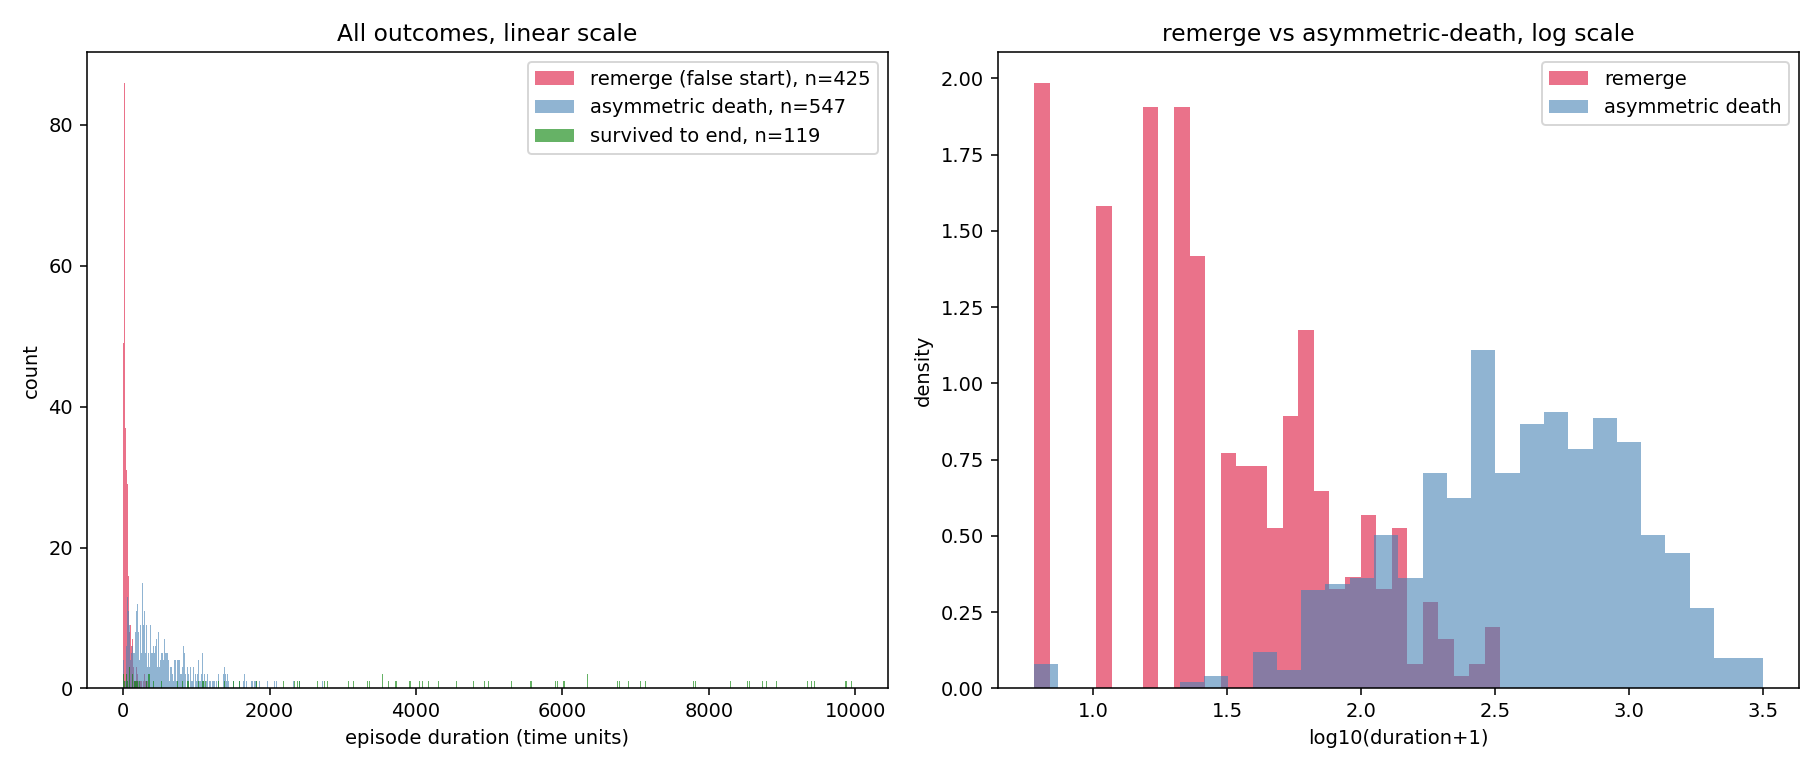
\includegraphics[width=0.75\textwidth]{split_duration_histogram.png}
\caption{Exploratory pass with no confirmation window, used to select the 50-time-unit confirmation window applied in the final procedure (\S\ref{sec:falsestarts}). Left: duration of detected split episodes, by eventual outcome, linear scale. Right: the same two dominant outcomes only, log-duration scale, showing the separation more clearly. False starts (remerges) cluster at short durations; episodes ending in one child's later, independent death cluster at durations comparable to the organism lifespan.}
\label{fig:duration_hist}
\end{figure}

\subsection{Lifespan Distribution}
\label{sec:lifespan}

Using the confirmed-division lineage record at $1024\times1024$ (merge-fused organisms, pseudo-spectral solver, distance-transform interior definition), the population's lifespan distribution has median \nn{\LifeMedianAll} time units overall (median \nn{\LifeMedianDeath} for organisms that end in ordinary death and \nn{\LifeMedianDivision} for organisms that end by dividing; $N=\nn{\LifeCompleted}$ completed lifecycles; Figure~\ref{fig:lifespan}). The \nn{\LifeInitial} organisms already present at the start of the run have unknown true ages; excluding them leaves $N=\nn{\LifeKeptN}$ with medians \nn{\LifeKeptMedianAll} overall, \nn{\LifeKeptMedianDeath} for deaths and \nn{\LifeKeptMedianDivision} for divisions. The division-ending figure is longer than the $\sim$660 time-unit replication time reported by \citet{Pearson1993} for an isolated spot dividing into open, unoccupied territory---the expected direction of difference, since every division in our competitive population must reach the same growth threshold while sharing substrate with neighbours, which should slow growth relative to the unconstrained case.

\begin{figure}[htbp]
\centering
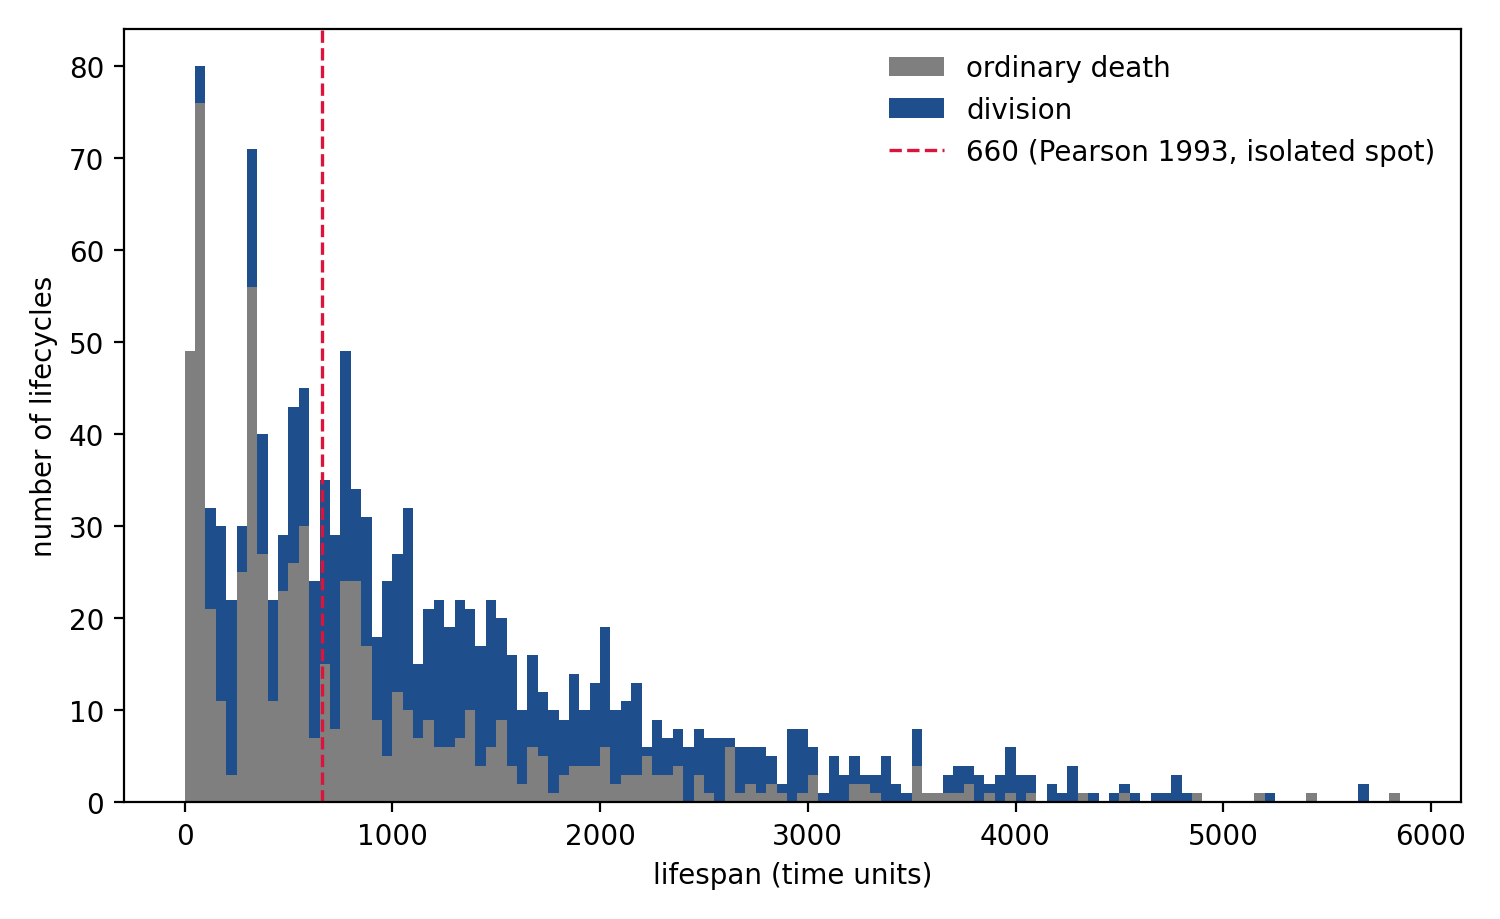
\includegraphics[width=0.8\textwidth]{lifespan_1024.png}
\caption{Lifespan distribution of confirmed organisms at $1024\times1024$, by cause of lifecycle termination (ordinary death vs.\ division). The reference line at 660 time units marks \citet{Pearson1993}'s isolated-spot replication time.}
\label{fig:lifespan}
\end{figure}

Early local crowding predicts an individual organism's time-to-division only weakly; see \S\ref{sec:S_crowding_division}.

\subsection{Autocorrelation Times of the States and Fluxes (Main Text \S\ref{sec:timescale})}
\label{sec:S_autocorr}

For each tracked lineage of merged organisms (the lifecycle tracker of this section) the series of $I$, $E$, $\Phi_u$ and $\Phi_v$ is demeaned, and the autocorrelation at lag $k$ is the sum over lineages of products of demeaned values $k$ samples apart, divided by the pooled variance of the same pairs. Fluxes are recorded every 5 time units and $I$, $E$ every 20. The autocorrelation time is the lag at which this pooled function first falls below $1/e$ (linear interpolation; script \texttt{analyze\_autocorr\_lifecycle.py}). It is about \rr{0}{\AcfTimeI} time units for $I$, \rr{0}{\AcfTimeE} for $E$, and \rr{0}{\AcfTimeFluxU} and \rr{0}{\AcfTimeFluxV} for $\Phi_u$ and $\Phi_v$, all well above $\tau\approx\rr{1}{\Tau}$. The blanket fluxes are slower than $I$ but not slower than $E$, so the strict form of Friston's criterion, a blanket that changes more slowly than the states it separates, is unestablished in either direction. The sampling intervals differ between variables, so the comparison is approximate.

\section{Further Exploratory Checks and Estimator-Calibration Detail (Main Text \S\ref{sec:timescale}, \S\ref{sec:alt_explanations}, \S\ref{sec:limitations})}
\label{sec:S_further_checks}

\subsection{Early Crowding and Time-to-Division}
\label{sec:S_crowding_division}

We asked whether local crowding predicts an individual organism's time-to-division, beyond the aggregate comparison to Pearson's isolated-spot figure. This requires care: a naive measurement of nearest-neighbour distance at the \emph{instant} of division is confounded by the organism's own size at that instant (an organism is largest, and hence appears closest to its neighbours by simple geometry, exactly when it is about to divide), and crowding averaged over an organism's \emph{entire}, variable-length lifetime produces a reverse-dependency artefact, since a longer-lived organism has more time for its local neighbourhood to change independent of any causal effect of crowding on its own growth rate. We therefore fix the measurement window to a common duration, the first 100 time units after birth, for every organism regardless of eventual lifespan. At $1024\times1024$ with merge-fused organisms this gives no detectable effect of early crowding on time-to-division ($r=\rr{3}{\CrowdR}$, 95\% CI $[\rr{3}{\CrowdLo},\rr{3}{\CrowdHi}]$, $N=\nn{\CrowdN}$), so most of the variance in time-to-division is evidently governed by something other than early crowding.

\subsection{Linear Stability of the Local Kinetics at Organism Boundaries and Cores (Main Text \S\ref{sec:timescale})}
\label{sec:S_jacobian}

The main text normalises boundary motion by the relaxation time of the background state, because the kinetics at an organism's own boundary are locally growing rather than relaxing. Whether they are growing is a property of the full, coupled $(u,v)$ Jacobian, not simply the sign of $2uv-(F+k)$, the diagonal element of $\partial(\partial v/\partial t)/\partial v$: a positive diagonal term does not by itself guarantee a growing mode of the coupled system, since the off-diagonal coupling and $u$'s own decay can stabilise it. The local reaction Jacobian of Eqs.~\ref{eq:gs_u}--\ref{eq:gs_v} is
\begin{equation}
J(u,v) = \begin{pmatrix} -F - v^2 & -2uv \\ v^2 & -F-k+2uv \end{pmatrix},
\end{equation}
and we evaluated its eigenvalues directly on real $(u,v)$ pairs sampled from one archived $1024\times1024$ frame (frame \nn{\JacFrame} of the single trajectory: \nn{\JacUsed} organisms, each with a non-empty boundary ring and core; script \texttt{check\_\allowbreak local\_\allowbreak jacobian.py}), separately at each organism's boundary (a thin ring just inside the watershed contour) and its eroded core. The diagonal criterion $2uv>F+k$ is satisfied at essentially every sampled location, boundary and core alike (mean boundary $u=\rr{2}{\JacBoundaryU}$, $v=\rr{2}{\JacBoundaryV}$; mean core $u=\rr{2}{\JacCoreU}$, $v=\rr{2}{\JacCoreV}$)---but the full-Jacobian eigenvalues tell a materially different story. \rr{0}{\JacBoundaryPositivePercent}\% of the \nn{\JacUsed} sampled organism boundaries have a genuinely positive dominant eigenvalue (median \rr{4}{\JacBoundaryMedian}), confirming a real growing mode exactly where $\rho$'s denominator needs one; but only \rr{0}{\JacCorePositivePercent}\% of organism cores do, \rr{0}{\JacCoreStablePercent}\% showing a complex-conjugate pair with negative real part---locally stable, damped-oscillatory kinetics, not growing ones. That the kinetics have no stable local relaxation rate of their own is therefore accurate specifically at the boundary, which is what $\tau$ is being used to normalise; it should not be read as a claim about organism interiors generally, where the diagonal-only criterion overstates instability.

\subsection{Shape Stability and the Shape-Correlation Tail (Main Text \S\ref{sec:timescale})}
\label{sec:S_shape_tail}

The shape descriptor is each organism's boundary contour resampled onto a 64-point angular grid about its centroid; consecutive frames (10 steps apart) are compared by the best-aligning circular rotation, for unambiguously matched organisms only. The analysis uses the same merge-corrected individuation as the rest of the paper (marker spacing 24), on \nn{\FramesShapeTail} frames of the settled $1024^2$ trajectory (\nn{\ShapeN} matched transitions; \texttt{run\_shape\_stability.py}, then \texttt{run\_shape\_tail\_test.py} for the decomposition below). The correlation has median \rr{3}{\ShapeCorrMedian}, mean \rr{3}{\ShapeCorrMean}, 10th percentile \rr{3}{\ShapeCorrTenth} and 1st percentile \rr{3}{\ShapeCorrFirst}. To ask what produces the low-correlation tail we also computed an amplitude measure, the root-mean-square difference of $r(\theta)$ between frames (best rotation) as a fraction of the organism's radius, and tagged every transition by how the organism's track ends and how many frames away that is.

\paragraph{The correlation tail is mostly a property of nearly circular organisms.} Splitting organisms into fifths by anisotropy, $\mathrm{std}(r)/\mathrm{mean}(r)$, the fraction of transitions below the correlation of $0.667$ is \rr{1}{\ShapeTailAnisOne}\%, \rr{1}{\ShapeTailAnisTwo}\%, \rr{1}{\ShapeTailAnisThree}\%, \rr{1}{\ShapeTailAnisFour}\% and \rr{1}{\ShapeTailAnisFive}\% from the most circular fifth to the most elongated. Splitting by radius, the rate falls from \rr{1}{\ShapeTailRadOne}\% (smallest fifth) to \rr{1}{\ShapeTailRadFive}\% (largest). Of the transitions in the tail, \rr{0}{\ShapeTailSmallChangePercent}\% change the boundary by less than $5\%$ of the radius, and \rr{0}{\ShapeTailNotDivisionPercent}\% are neither division, pre-division nor post-division transitions. A low rotation-aligned correlation therefore mainly says that there is little non-circular shape to correlate, not that the boundary is moving.

\paragraph{Amplitude of shape change.} The median change is \rr{1}{\ShapeRmsMedianPercent}\% of the radius, the 90th percentile \rr{1}{\ShapeRmsNinetiethPercent}\% and the 99th \rr{1}{\ShapeRmsNinetyNinthPercent}\%; \rr{1}{\ShapeRmsBelowFivePercent}\% of transitions change by less than $5\%$ and \rr{1}{\ShapeRmsBelowTenPercent}\% by less than $10\%$.

\paragraph{Where the large changes are.} Among the top 1\% of amplitude changes (above \rr{1}{\ShapeBigThresholdPercent}\% of the radius, $n=\nn{\ShapeBigN}$): \rr{1}{\ShapeBigDivisionShare}\% are the division transition itself (\rr{0}{\ShapeDivisionAboveBig}\% of the \nn{\ShapeDivisions} division transitions exceed this value); \rr{1}{\ShapeBigDeathShare}\% fall within five frames before the organism disappears, where \rr{1}{\ShapeBigDeathRate}\% of such transitions are large (median amplitude \rr{3}{\ShapeBigDeathMedian}, $n=\nn{\ShapeBigDeathN}$); \rr{1}{\ShapeBigAmbigShare}\% fall within five frames before the track ends without a clean successor (less than half overlap, or no usable contour), \rr{1}{\ShapeBigAmbigRate}\% of such transitions being large (median \rr{3}{\ShapeBigAmbigMedian}, $n=\nn{\ShapeBigAmbigN}$); and \rr{1}{\ShapeBigMergeShare}\% fall within five frames before a merge (rate \rr{1}{\ShapeBigMergeRate}\%, median \rr{3}{\ShapeBigMergeMedian}, $n=\nn{\ShapeBigMergeN}$). Transitions in the five frames before a division are almost never large (rate \rr{1}{\ShapePreBigRate}\%, median correlation \rr{3}{\ShapePreCorrMedian}). Large shape changes are thus concentrated at division and in the last few frames of an organism's life, and are not associated with merging.

\subsection{CMI Null Calibration and the Scale-Sensitivity Artefact (Main Text \S\ref{sec:limitations})}
\label{sec:S_cmi_calibration}

\paragraph{Calibration of the two nulls.} The CMI test (main text \S\ref{sec:blanket}) uses two nulls: a 30-group within-cluster shuffle, and a local nearest-neighbour swap in the style of \citet{Runge2018} (10 neighbours), which conditions on $\bB{}$ far more finely and is the headline null. We checked both on the data of this paper, using a surrogate in which $I\perp E\mid\bB{}$ holds exactly. Random-forest regressions $\hat\mu_I(\bB{})$ and $\hat\mu_E(\bB{})$ were fitted to the real organism instances (surrogate $R^2$ of $I$ on $\bB{}$ $=\rr{3}{\CalRsqI}$; of $E$ on $\bB{}$ $=\rr{3}{\CalRsqE}$). Each replicate keeps the real $\bB{}$ values and fitted means and adds two independently permuted draws of the real residual pools, so the real marginal shapes and the real nonlinear $\bB{}$-dependence are preserved while any further $I$--$E$ dependence is destroyed. We ran \nn{\CalReplicates} replicates ($N=\nn{\CalSub}$ each, all variables $z$-scored, \nn{\CalNull} null trials per null; \texttt{run\_null\_calibration.py}). For a calibrated null, $z=(\text{observed}-\text{null mean})/\text{null SD}$ should have mean 0 and SD 1:
\begin{center}\small
\begin{tabular}{lcccc}
\hline
Null & $z$ mean & $z$ SD & $P(z>1.645)$ & $P(z>1.96)$\\
\hline
30-group & \rr{2}{\CalClusterZMean} & \rr{2}{\CalClusterZSD} & \rr{3}{\CalClusterOverLowFrac} & \rr{3}{\CalClusterOverHighFrac}\\
Local nearest-neighbour & \rr{2}{\CalLocalZMean} & \rr{2}{\CalLocalZSD} & \rr{3}{\CalLocalOverLowFrac} & \rr{3}{\CalLocalOverHighFrac}\\
\hline
\end{tabular}
\end{center}
The mean excess over the null was \rr{4}{\CalClusterExcessMean} nats (30-group, SD \rr{4}{\CalClusterExcessSD}) and \rr{4}{\CalLocalExcessMean} nats (local, SD \rr{4}{\CalLocalExcessSD}). Both nulls therefore have close to the nominal type-I error. With \nn{\CalReplicates} replicates the fractions are known only to about $\pm3$ percentage points, so this is a check against gross miscalibration, not a precise size estimate. It covers the conditional-independence structure we constructed, not every way the real system might differ from it.

\paragraph{Cross-check against an independent implementation.} The estimator is our own implementation of the Frenzel--Pompe formula (\texttt{conditional\_mi.py}). We compared it with the \texttt{CMIknn} estimator of Tigramite \texttt{\TigVersion} \citep{Runge2018} on the real data (\texttt{run\_cmi\_crosscheck.py}): \nn{\TigSeeds} $N=\nn{\TigSub}$ subsamples of the master dataset, $k_{\mathrm{NN}}=5$, blankets with $w=0$ (flux alone), $8$ and $24$ px, all variables $z$-scored. Tigramite's default preprocessing is a rank transform, so the main comparison sets it to standardise. The two estimators then agree to within \rr{4}{\TigZeroMaxDiff}, \rr{4}{\TigEightMaxDiff} and \rr{4}{\TigTwentyFourMaxDiff} nats in every subsample (means over the subsamples \rr{4}{\TigZeroOurs}, \rr{4}{\TigEightOurs} and \rr{4}{\TigTwentyFourOurs} nats for $w=0$, $8$, $24$). With Tigramite's default rank transform the values are \rr{4}{\TigZeroRank}, \rr{4}{\TigEightRank} and \rr{4}{\TigTwentyFourRank}, the same pattern with \rr{0}{\TigZeroRankLowPercent}\% lower values for flux alone. For flux alone, Tigramite's own local-permutation null (10 neighbours, \nn{\TigNullTrials} trials, first subsample) has mean \rr{4}{\TigNullMean} and SD \rr{4}{\TigNullSD} against \rr{4}{\TigOursNullMean} and \rr{4}{\TigOursNullSD} for ours, which puts the observed value \rr{1}{\TigExcessTig} SDs above the null against \rr{1}{\TigExcessOurs}.

\paragraph{Scale sensitivity of the estimator.} The nearest-neighbour CMI estimator uses a max-norm search, so it is sensitive to the numerical range of its inputs. Blanket flux ($\sim10^{-4}$) is three orders of magnitude smaller than $I$ and $E$ ($\sim10^{-1}$), so on raw inputs the neighbour distance is set almost entirely by $I$ and $E$ and the estimator stops meaningfully conditioning on flux; multiplying flux alone by $10^4$, with nothing else changed, moves the estimate substantially. All CMI figures in this paper therefore $z$-score $I$, $E$, $\Phi_u$ and $\Phi_v$ before estimation, identically for the observed statistic and every null trial. With the merge-based segmentation this raises the observed CMI from \rr{3}{\ScaleEnsRaw} to \rr{3}{\ScaleEnsZ} nats on the ensemble and from \rr{3}{\ScaleTrajRaw} to \rr{3}{\ScaleTrajZ} nats on the single trajectory (on a single $N=\nn{\ScaleNSub}$ subsample of each; multiplying flux alone by $10^4$ gives \rr{3}{\ScaleEnsTimes} and \rr{3}{\ScaleTrajTimes}), and the nearest-neighbour null mean is about \rr{3}{\ScaleEnsNullMean} nats (SD \rr{3}{\ScaleEnsNullSD}). The primary figures are computed on matched $N=\nn{\CmiNSub}$ subsamples of both datasets, since the nearest-neighbour search is also very slow at full size.

\section{Computational Reproducibility}
\label{sec:S_reproducibility}

This section lists, for every simulation-dependent quantity in the main text and this supplement, the script that produces it and the command used to run it, so that any reported number can be regenerated. All scripts are distributed alongside this paper's code and data (\url{https://github.com/johnepearson/GS_FEP}; see also main text, Data Accessibility) and run from a single directory (\texttt{local\_package/}) containing \texttt{checkpoint\_1024\_settled.npz}, a pre-relaxed $1024\times1024$ field. The file records \nn{\SettleSteps} time units of evolution and holds about 185 organisms; the initial condition it was grown from was not recorded, so it is distributed as data. Wall-clock times are for a 2024 MacBook Pro (12 cores) and are given only where they were measured. Unless noted, all individuation uses the merge-corrected watershed with marker spacing 24 pixels (\S\ref{sec:individuation}). The single-trajectory run archives every field (\texttt{master\_fields/}) so that follow-up analyses need no new simulation; the ensembles and the lifecycle tracker are independent simulations. The ensembles are the only stochastic runs (their random seeds are fixed by \texttt{--seed-base}); the single-trajectory and lifecycle runs are deterministic.

\paragraph{The C solver.} The production runs ($1024\times1024$, the \texttt{--fast} option of the scripts) use a C implementation of the pseudo-spectral scheme of \S\ref{sec:S_pseudospectral} (\texttt{gs\_spectral\_c.c}, loaded by \texttt{gray\_scott\_spectral\_c.py}). It keeps the state in Fourier space and needs three FFTs per step instead of six, using FFTW3 with its threaded library; it needs a C compiler and is not distributed pre-built, since the library path is platform-specific. The pure-Python solver (\texttt{gray\_scott\_spectral.py}) implements the same update and the same spectral layout, but transforms $u$, $v$, $R_u$ and $R_v$ separately (six FFTs per step) and can replace it, at about $2.5$--$3$ times the run time on 2 cores and about $4$ times on a 12-core laptop. We checked the two against each other (\texttt{check\_c\_solver.py}): from the settled $1024\times1024$ checkpoint, the largest difference in $u$ or $v$ is $1.3\times10^{-15}$ after 10 steps, $1.2\times10^{-14}$ after 100, $7\times10^{-12}$ after 1{,}000, $6\times10^{-11}$ after 2{,}000, $8\times10^{-9}$ after 3{,}000 and $3\times10^{-7}$ after 4{,}000 steps. Repeating the check on the 12-core laptop gives the same numbers to within a factor of about 1.2 ($1.4\times10^{-15}$, $8.8\times10^{-15}$, $8.5\times10^{-12}$, $7.2\times10^{-11}$, $7.6\times10^{-9}$, $3.0\times10^{-7}$ at 10, 100, 1{,}000, 2{,}000, 3{,}000, 4{,}000 steps). The two agree to rounding error, and the difference then grows slowly, as any rounding-level perturbation does in this chaotic system (the growth is comparable to that of the noise-perturbed pairs of \S\ref{sec:S_robustness}). Individual trajectories from the two solvers will therefore drift apart after several thousand steps, as they would for two runs with different thread counts, which is why the paper's statistics are checked across independent ensembles and not tied to one trajectory. Build commands:
\begin{quote}\footnotesize
\begin{verbatim}
macOS (Homebrew):  brew install fftw
  gcc -O3 -march=native -fPIC -shared -o libgs_spectral.so gs_spectral_c.c \
      -I$(brew --prefix fftw)/include -L$(brew --prefix fftw)/lib \
      -lfftw3_threads -lfftw3 -lpthread -lm
Debian/Ubuntu:     sudo apt-get install -y libfftw3-dev
  gcc -O3 -march=native -fPIC -shared -o libgs_spectral.so gs_spectral_c.c \
      -lfftw3_threads -lfftw3 -lpthread -lm
\end{verbatim}
\end{quote}

{\small
\begin{longtable}{>{\raggedright\arraybackslash}p{3.9cm}>{\raggedright\arraybackslash}p{3.9cm}>{\raggedright\arraybackslash}p{4.6cm}>{\raggedright\arraybackslash}p{2.3cm}}
\toprule
Quantity (paper location) & Script & Command & Time \\
\midrule
\endfirsthead
\toprule
Quantity (paper location) & Script & Command & Time \\
\midrule
\endhead
\bottomrule
\endfoot
\bottomrule
\caption{Reproducibility table: script and command for each simulation-dependent quantity. ``Master'' is \texttt{master\_\allowbreak trajectory\_\allowbreak progress.npz} (\nn{\MasterFrames} frames, 100 solver steps apart, $N=\nn{\TrajN}$ organism-instances) together with the archived fields in \texttt{master\_\allowbreak fields/}.}
\label{tab:S_repro_table}\\
\endlastfoot

Single trajectory: all organism-level data ($I$, $E$, fluxes, radius, eccentricity, shells, boundary values, merge size) &
\texttt{run\_\allowbreak master\_\allowbreak trajectory.py} &
\texttt{python3 run\_\allowbreak master\_\allowbreak trajectory.py --n-\allowbreak frames \MasterFrames\ --fast} &
about 1--1.5 h \\
\addlinespace
Single-trajectory statistics, collinearity and confound checks, frame fixed effects, richer-blanket check, nonlinear CMI (\S\ref{sec:conditional_independence}, \S\ref{sec:alt_explanations}, \S\ref{sec:richer_blanket}; ESM \S\ref{sec:S_alt_explanations}, \S\ref{sec:S_mechanism_scope}) &
\texttt{analyze\_\allowbreak master.py}, \texttt{analyze\_\allowbreak master\_\allowbreak followups.py}, \texttt{analyze\_\allowbreak pooled\_\allowbreak collider\_\allowbreak cmi.py} &
\texttt{python3 analyze\_\allowbreak master.py}; \texttt{python3 analyze\_\allowbreak master\_\allowbreak followups.py}; \texttt{python3 analyze\_\allowbreak pooled\_\allowbreak collider\_\allowbreak cmi.py --seeds 0 1 2 --data master\_\allowbreak trajectory\_\allowbreak progress.npz} (full-population collider CMI, about 10 min) &
--- \\
\addlinespace
Radius/eccentricity diagnostics (ESM \S\ref{sec:S_alt_explanations}) &
\texttt{diag\_\allowbreak size\_\allowbreak shape.py}, \texttt{diag\_\allowbreak size\_\allowbreak shape2.py}, \texttt{radius\_\allowbreak flux\_\allowbreak share.py} &
\texttt{python3 diag\_\allowbreak size\_\allowbreak shape.py}; \texttt{python3 diag\_\allowbreak size\_\allowbreak shape2.py}; \texttt{python3 radius\_\allowbreak flux\_\allowbreak share.py} &
$<$1 min \\
\addlinespace
Depth sensitivity (ESM \S\ref{sec:S_ci_support}) &
\texttt{sweep\_\allowbreak from\_\allowbreak master.py}, \texttt{plot\_\allowbreak depth\_\allowbreak sensitivity\_\allowbreak pc1.py} &
\texttt{python3 sweep\_\allowbreak from\_\allowbreak master.py --stride \DepthStride} &
--- \\
\addlinespace
Independent ensembles, \nn{\RunsOne} realisations each, seeds \SeedOne\ and \SeedTwo (\S\ref{sec:ci_ensemble}, Figure~\ref{fig:ensemble_summary}, \S\ref{sec:friston_fe}) &
\texttt{run\_\allowbreak ensemble\_\allowbreak merged.py}, \texttt{analyze\_\allowbreak ensemble\_\allowbreak merged.py} &
\texttt{for i in \$(seq 0 11); do GS\_\allowbreak FFT\_\allowbreak THREADS=1 python3 run\_\allowbreak ensemble\_\allowbreak merged.py --n-\allowbreak realizations \RunsOne\ --n-\allowbreak workers \CmiJobs\ --worker-id \$i --fast --seed-base \SeedOne\ --burn-in-steps \BurninOne \& done; wait} (seed \SeedTwo\ for the second set; for the third set use seed \SeedThree\ with \RunsThree\ realisations and \texttt{--burn-in-steps \BurninThree}, then \texttt{python3 analyze\_\allowbreak ensemble\_\allowbreak pc1.py}) &
2 h 19 min and 2 h 43 min for the two sets of 1000 realisations (a previous run) \\
\addlinespace
Slice and conditional-MI summary figure (Figure~\ref{fig:ensemble_summary}) &
\texttt{plot\_\allowbreak ensemble\_\allowbreak summary.py} &
\texttt{python3 plot\_\allowbreak ensemble\_\allowbreak summary.py} (reads \texttt{ensemble\_\allowbreak merged\_\allowbreak seed1000\_\allowbreak worker*.npz}; uses every organism in each flux group; \texttt{--subsample 3000} gives random 3000-point draws instead) &
$\approx$ 10 min \\
\addlinespace
Blanket-thickness and substrate-enriched figures (Figures~\ref{fig:S_band} and~\ref{fig:S_u_enriched}) &
\texttt{plot\_\allowbreak blanket\_\allowbreak figures.py} &
\texttt{python3 plot\_\allowbreak blanket\_\allowbreak figures.py} (reads \texttt{run\_\allowbreak band\_\allowbreak sweep\_\allowbreak seed0.npz} to \texttt{seed2.npz} and \texttt{u\_\allowbreak enriched\_\allowbreak cmi\_\allowbreak ring.npz}) &
seconds \\
\addlinespace
Friston generative-model fit (\S\ref{sec:friston_fe}) &
\texttt{rebuild\_\allowbreak fig5\_\allowbreak and\_\allowbreak fe\_\allowbreak model.py}; shared constants in \texttt{fe\_\allowbreak model.py} &
\texttt{python3 rebuild\_\allowbreak fig5\_\allowbreak and\_\allowbreak fe\_\allowbreak model.py} (\texttt{fe\_\allowbreak model.py} refits and caches on first use) &
$<$ 5 min \\
\addlinespace
Timescale separation, flux asymmetry, boundary mechanism (\S\ref{sec:timescale}, \S\ref{sec:flux}) &
\texttt{run\_\allowbreak remaining\_\allowbreak checks\_\allowbreak merged.py}, \texttt{plot\_\allowbreak timescale\_\allowbreak flux\_\allowbreak merged.py} &
\texttt{python3 run\_\allowbreak remaining\_\allowbreak checks\_\allowbreak merged.py --n-\allowbreak frames \FramesRemaining}; \texttt{python3 plot\_\allowbreak timescale\_\allowbreak flux\_\allowbreak merged.py --data remaining\_\allowbreak checks\_\allowbreak merged\_\allowbreak md24\_\allowbreak results.npz} &
--- \\
\addlinespace
Shape stability and the shape-correlation tail (\S\ref{sec:timescale}; ESM \S\ref{sec:S_shape_tail}) &
\texttt{run\_\allowbreak shape\_\allowbreak stability.py}, \texttt{run\_\allowbreak shape\_\allowbreak tail\_\allowbreak test.py} &
\texttt{python3 run\_\allowbreak shape\_\allowbreak tail\_\allowbreak test.py --n-\allowbreak frames \FramesShapeTail} (imports the shape functions from \texttt{run\_\allowbreak shape\_\allowbreak stability.py}) &
$\approx$ 8 min \\
\addlinespace
Local-kinetics Jacobian eigenvalues at boundaries and cores, and $1/(F+k)$ (ESM \S\ref{sec:S_jacobian}) &
\texttt{check\_\allowbreak local\_\allowbreak jacobian.py} &
\texttt{python3 check\_\allowbreak local\_\allowbreak jacobian.py --frame \JacobianFrame} (reads \texttt{master\_\allowbreak fields/}) &
seconds \\
\addlinespace
C solver agreement with the Python solver (ESM \S\ref{sec:S_reproducibility}) &
\texttt{check\_\allowbreak c\_\allowbreak solver.py} &
\texttt{python3 check\_\allowbreak c\_\allowbreak solver.py} (needs \texttt{libgs\_\allowbreak spectral.so}, built as described above) &
minutes \\
\addlinespace
CMI estimator cross-check against Tigramite (ESM \S\ref{sec:S_cmi_calibration}) &
\texttt{run\_\allowbreak cmi\_\allowbreak crosscheck.py} &
\texttt{python3 -m pip install tigramite numba}; \texttt{python3 run\_\allowbreak cmi\_\allowbreak crosscheck.py} &
minutes \\
\addlinespace
CMI on subsamples without same-frame coupling (ESM \S\ref{sec:S_robustness}) &
\texttt{run\_\allowbreak cmi\_\allowbreak independent\_\allowbreak frames.py} &
\texttt{python3 run\_\allowbreak cmi\_\allowbreak independent\_\allowbreak frames.py --data ensemble:\SeedOne\ --jobs \CmiJobs}; \texttt{python3 run\_\allowbreak cmi\_\allowbreak independent\_\allowbreak frames.py --data master --jobs \CmiJobs} &
$\approx$ 1 min each \\
\addlinespace
Placebo-disk blanket-thickness sweep (\S\ref{sec:richer_blanket}; ESM \S\ref{sec:S_band}) &
\texttt{run\_\allowbreak random\_\allowbreak disks.py}, \texttt{run\_\allowbreak band\_\allowbreak sweep\_\allowbreak cmi.py} &
\texttt{python3 run\_\allowbreak random\_\allowbreak disks.py --stride 3 --jobs 12}; \texttt{python3 run\_\allowbreak band\_\allowbreak sweep\_\allowbreak cmi.py --data random\_\allowbreak disks.npz --tag \_disks --only-\allowbreak all --jobs 12} (reads \texttt{master\_\allowbreak fields/}) &
$\approx$ 11 min \\
\addlinespace
Resolution $\times$ interior-definition factorial (\S\ref{sec:model}; ESM \S\ref{sec:S_resolution_factorial}) &
\texttt{run\_\allowbreak resolution\_\allowbreak 2x2\_\allowbreak merged.py}, \texttt{analyze\_\allowbreak resolution\_\allowbreak 2x2\_\allowbreak merged.py} &
\texttt{python3 run\_\allowbreak resolution\_\allowbreak 2x2\_\allowbreak merged.py --resolution 256 --n-\allowbreak frames 400}; \texttt{... --resolution 1024 ...}; then \texttt{python3 analyze\_\allowbreak resolution\_\allowbreak 2x2\_\allowbreak merged.py} &
--- \\
\addlinespace
Lifecycle tracker: confirmed divisions, deaths, lifespans, crowding vs.\ time-to-division (\S\ref{sec:fe_comparison}; ESM \S\ref{sec:S_lineage}) &
\texttt{run\_\allowbreak lifecycle.py}, \texttt{analyze\_\allowbreak lifecycle.py} &
\texttt{python3 run\_\allowbreak lifecycle.py --n-\allowbreak steps \LifeSteps\ --fast}; \texttt{python3 analyze\_\allowbreak lifecycle.py} &
20 min (1181\,s) \\
\addlinespace
Autocorrelation times of $I$, $E$, $\Phi_u$, $\Phi_v$ (main text \S\ref{sec:timescale}; ESM \S\ref{sec:S_autocorr}) &
\texttt{analyze\_\allowbreak autocorr\_\allowbreak lifecycle.py} &
\texttt{python3 analyze\_\allowbreak autocorr\_\allowbreak lifecycle.py} (reads \texttt{lifecycle\_\allowbreak progress.pkl}) &
seconds \\
\addlinespace
Age-confound and lineage fixed-effects checks (\S\ref{sec:alt_explanations}; ESM \S\ref{sec:S_alt_explanations}) &
\texttt{analyze\_\allowbreak lifecycle\_\allowbreak age.py}, \texttt{run\_\allowbreak lineage\_\allowbreak mixture\_\allowbreak decomposition.py} &
\texttt{python3 analyze\_\allowbreak lifecycle\_\allowbreak age.py}; \texttt{python3 run\_\allowbreak lineage\_\allowbreak mixture\_\allowbreak decomposition.py} (reads \texttt{lifecycle\_\allowbreak progress.pkl}, then \texttt{lifecycle\_\allowbreak age\_\allowbreak analysis.npz}) &
$\approx$ 6 min \\
\addlinespace
Radial template $T(r)$ from merged organisms of the single trajectory (\S\ref{sec:template_fe}; ESM \S\ref{sec:S_template_procedure}) &
\texttt{build\_\allowbreak template\_\allowbreak from\_\allowbreak master.py} &
\texttt{python3 build\_\allowbreak template\_\allowbreak from\_\allowbreak master.py} &
minutes \\
\addlinespace
Free-energy comparison, Figure~\ref{fig:fe_comparison}; instance-level, held-out-template and split-half checks (\S\ref{sec:fe_comparison}; ESM \S\ref{sec:S_fe_comparison}) &
\texttt{check\_\allowbreak flux\_\allowbreak massbalance.py} (\S\ref{sec:S_uv2_flux}), \texttt{analyze\_\allowbreak uv2\_\allowbreak lifecycle.py} (Figure~\ref{fig:fe_comparison}, the $uv^2$ curves and the correlations quoted with it; needs a tracker run of \texttt{run\_\allowbreak lifecycle.py} that records $uv^2$, its total and the area), \texttt{analyze\_\allowbreak surprisal.py} (\S\ref{sec:S_surprisal}), \texttt{pc1\_\allowbreak details.py} (\S\ref{sec:S_pc1}), \texttt{run\_\allowbreak band\_\allowbreak sweep\_\allowbreak cmi.py} (\S\ref{sec:S_band}; \texttt{python run\_band\_sweep\_cmi.py --jobs 12 --seed 0}), \texttt{run\_\allowbreak u\_\allowbreak enriched\_\allowbreak cmi.py} (\S\ref{sec:S_u_enriched}; \texttt{python run\_u\_enriched\_cmi.py --jobs 12}, then again with \texttt{--target far}), \texttt{rebuild\_\allowbreak fe\_\allowbreak comparison\_\allowbreak 1024.py}, \texttt{rebuild\_\allowbreak instance\_\allowbreak level\_\allowbreak check.py}, \texttt{rebuild\_\allowbreak circularity\_\allowbreak check\_\allowbreak v2.py}, \texttt{rebuild\_\allowbreak splithalf\_\allowbreak check.py} &
\texttt{python3 <script>} for each, in \texttt{local\_\allowbreak package/} &
$<$ 5 min each \\
\addlinespace
Free-energy size control (ESM \S\ref{sec:S_fe_comparison}) &
\texttt{run\_\allowbreak fe\_\allowbreak size\_\allowbreak control.py} &
\texttt{python3 run\_\allowbreak fe\_\allowbreak size\_\allowbreak control.py} &
minutes \\
\addlinespace
Moving-block bootstrap, single trajectory (ESM \S\ref{sec:S_robustness}) &
\texttt{run\_\allowbreak block\_\allowbreak bootstrap\_\allowbreak master.py} &
\texttt{python3 run\_\allowbreak block\_\allowbreak bootstrap\_\allowbreak master.py} &
under 5 min \\
\addlinespace
CMI null calibration on the current data (ESM \S\ref{sec:S_cmi_calibration}) &
\texttt{run\_\allowbreak null\_\allowbreak calibration.py} &
\texttt{python3 run\_\allowbreak null\_\allowbreak calibration.py --n-rep \NullReps\ --jobs \CmiJobs} &
about 5 min \\
\addlinespace
Level-set individuation comparison (\S\ref{sec:levelset}; ESM \S\ref{sec:S_levelset}) &
\texttt{level\_\allowbreak set\_\allowbreak from\_\allowbreak master.py}, \texttt{run\_\allowbreak levelset\_\allowbreak cmi.py} &
\texttt{python3 level\_\allowbreak set\_\allowbreak from\_\allowbreak master.py}; \texttt{python3 run\_\allowbreak levelset\_\allowbreak cmi.py --jobs 12} &
minutes \\
\addlinespace
Three-variable memory model, correlation length (\S\ref{sec:threevar_blanket}; ESM \S\ref{sec:S_threevar_impl}) &
\texttt{run\_\allowbreak 3var\_\allowbreak shell\_\allowbreak data.py}, \texttt{analyze\_\allowbreak 3var\_\allowbreak shells.py} &
\texttt{python3 run\_\allowbreak 3var\_\allowbreak shell\_\allowbreak data.py --dw 1e-5 --target-\allowbreak n \ThreeVarTarget}; \texttt{python3 run\_\allowbreak 3var\_\allowbreak shell\_\allowbreak data.py --dw 0.0 --target-\allowbreak n \ThreeVarTarget}; then \texttt{python3 analyze\_\allowbreak 3var\_\allowbreak shells.py} &
2 h 55 min ($D_w=D_v$), 1 h 54 min ($D_w=0$) \\
\addlinespace
Population-count decorrelation (ESM \S\ref{sec:S_robustness}) &
\texttt{run\_\allowbreak count\_\allowbreak decorrelation.py}, \texttt{analyze\_\allowbreak count\_\allowbreak decorrelation.py} &
\texttt{python3 run\_\allowbreak count\_\allowbreak decorrelation.py --n-\allowbreak real \CountReal\ --steps \CountSteps}; \texttt{python3 analyze\_\allowbreak count\_\allowbreak decorrelation.py} &
56 min \\
\addlinespace
Merge-correction illustration, Figure~\ref{fig:merge_correction} (ESM \S\ref{sec:S_merge_procedure}) &
\texttt{make\_\allowbreak merge\_\allowbreak figure.py} &
\texttt{python3 make\_\allowbreak merge\_\allowbreak figure.py [--pick N]} &
$\sim$2 s \\

\end{longtable}
}

\paragraph{Individuation used by each check.} The fixed-radius individuation and migration checks use marker spacing 32; they do not depend on how organisms are individuated. The three-variable memory model (\S\ref{sec:threevar}) uses spacing 24. The level-set comparison (\S\ref{sec:levelset}) is computed on the archived single-trajectory fields (\texttt{level\_set\_from\_master.py}).

\subsection{Template-Sampling Procedure for $\mathcal{F}_{\text{template}}$}
\label{sec:S_template_procedure}

The radial template $T(r)$ used by the template-deviation free energy (main text \S\ref{sec:template_fe}) is built by \texttt{build\_template\_from\_master.py}: for every merge-fused organism in each of the \nn{\MasterFrames} archived frames of the single-trajectory run ($N=\nn{\TrajN}$), it computes the radial profile of $v$ about the organism's periodic centroid (20 bins, 0--80 pixels), pools the profiles without conditioning on division status, and averages bin by bin to obtain $T(r)$ (also recording the per-bin standard deviation for the template figure's spread band). The single-trajectory run is a separate simulation from the lifecycle tracker's, so the template is independent of the lifecycle data on which it is evaluated. The template is built from merged organisms, because at this marker spacing raw watershed regions include fragments of single organisms.

\bibliographystyle{plainnat}
\bibliography{references}

\end{document}
